% Tipe dokumen adalah report dengan satu kolom kertas A4 satu sisi.
% Ukuran font 12pt
\documentclass[12pt, a4, onecolumn, oneside, final]{report}

% Load konfigurasi LaTeX untuk tipe laporan thesis
\usepackage{ta}	

\usepackage{enumitem}
%\setlist[enumerate]{itemsep=1pt, topsep=1pt}

\titleformat{\section}
  {\normalfont\fontsize{12}{15}\bfseries}{\thesection}{1em}{}

\titleformat{\subsection}
  {\normalfont\fontsize{12}{15}\bfseries}{\thesubsection}{1em}{}

% Load konfigurasi khusus untuk laporan yang sedang dibuat
%-----------------------------------------------------------------------------%
% Informasi Mengenai Dokumen
%-----------------------------------------------------------------------------%
% 
% Judul laporan. 
\var{\judul}{Rancang Bangun Sistem \textit{FMCW} Radar Berbasis \textit{Software Defined Radio} dengan \textit{GNURadio} Untuk Mendeteksi Objek, Estimasi Jarak, dan Kecepatan}
% 
% Tulis kembali judul laporan, kali ini akan diubah menjadi huruf kapital
\Var{\Judul}{Rancang Bangun Sistem \textit{FMCW} Radar Berbasis \textit{Software Defined Radio} dengan \textit{GNURadio} Untuk Mendeteksi Objek, Estimasi Jarak, dan Kecepatan}
% 
% Tulis kembali judul laporan namun dengan bahasa Inggris
\var{\judulInggris}{Design of FMCW Radar Based on Software Defined Radio with GNURadio for Object Detection, Range Estimation, and Velocity}

\Var{\JudulInggris}{Design of FMCW Radar Based on Software Defined Radio with GNURadio for Object Detection, Range Estimation, and Velocity}

% 
% Tipe laporan, dapat berisi Skripsi, Tugas Akhir, Thesis, atau Disertasi
\var{\type}{Tugas Akhir}
% 
% Tulis kembali tipe laporan, kali ini akan diubah menjadi huruf kapital
\Var{\Type}{Tugas Akhir}
% 
% Tulis nama penulis 
\var{\penulis}{Bima Pancara Haryono Putra}
\var{\alamat}{Perum. Mega Asri, B-02}
\var{\tlp}{089699444339}
\var{\email}{bimapancara@student.telkomuniversity.ac.id}
% 
% Tulis kembali nama penulis, kali ini akan diubah menjadi huruf kapital
\Var{\Penulis}{Bima Pancara Haryono Putra}
% 
% Tulis NPM penulis
\var{\nim}{1101210528}
% 
% Tuliskan Kampus dimana penulis berada
\var{\kampus}{Surabaya}
\Var{\Kampus}{Surabaya}
% Tuliskan Fakultas dimana penulis berada
\Var{\Fakultas}{Fakultas Teknik Elektro}
\var{\fakultas}{Fakultas Teknik Elektro}
% 
% Tuliskan Program Studi yang diambil penulis
\Var{\Program}{Teknik Telekomunikasi}
\var{\program}{Teknik Telekomunikasi}
% 
% Tuliskan tahun publikasi laporan
\Var{\Tahun}{2024}
% 
% Tuliskan gelar yang akan diperoleh dengan menyerahkan laporan ini
\var{\gelar}{Sarjana Teknik}
% 
% Tuliskan tanggal pengesahan laporan, waktu dimana laporan diserahkan ke 
% penguji/sekretariat
\var{\tanggalPengesahan}{XX XXXX 20XX} 
% 
% Tuliskan tanggal keputusan sidang dikeluarkan dan penulis dinyatakan 
% lulus/tidak lulus
%\var{\tanggalLulus}{25 April 2015}
% 
% Tuliskan pembimbing 
\var{\pembimbingSatu}{Dr. Fannush Shofi Akbar, S.ST.}
\var{\nikSatu}{20910026}
\var{\pembimbingDua}{Risdilah Mimma Untsa, S.ST., M.T.}
\var{\nikDua}{20910025}
% 
% Alias untuk memudahkan alur penulisan paa saat menulis laporan
\var{\saya}{Penulis}

%-----------------------------------------------------------------------------%
% Judul Setiap Bab
%-----------------------------------------------------------------------------%
% 
% Berikut ada judul-judul setiap bab. 
% Silahkan diubah sesuai dengan kebutuhan. 
% 
\Var{\kataPengantar}{Kata Pengantar}
\Var{\babSatu}{Pendahuluan}
\Var{\babDua}{Tinjauan Pustaka}
\Var{\babTiga}{Metode Penelitian}
\Var{\babEmpat}{Hasil dan Analisis}
\Var{\babLima}{Simpulan dan Saran}


% Awal bagian penulisan laporan
\begin{document}

% Sampul Laporan

\begin{titlepage}
    \begin{center}      
        % judul thesis harus dalam 14pt Times New Roman
        \bo{\Judul} \\[0.55cm]
        
        \vspace*{1 cm}
        \textit{\bo{\JudulInggris}} \\[1.5cm]    
        % harus dalam 14pt Times New Roman
        %\bo{\Type}
        \textbf{TUGAS AKHIR}\\
        Diajukan untuk memenuhi salah satu syarat memperoleh gelar sarjana\\
        Dari Program Studi S1 Teknik Telekomunikasi \\
        Direktorat Kampus Surabaya \\
        Universitas Telkom

        \vspace*{1 cm}       
        % penulis dan npm
        Disusun oleh:\\
        \bo{\Penulis} \\
        \bo{\nim} \\

        \vspace*{1.0cm}
        
        \begin{figure}
            \begin{center}
                
\includegraphics[scale=1]{pics/pengantar/TelU.png}
            \end{center}
        \end{figure}
        \vspace*{1.0cm}
        % informasi mengenai fakultas dan program studi
        \bo{
            PROGRAM STUDI SARJANA TEKNIK TELEKOMUNIKASI\\
            DIREKTORAT KAMPUS SURABAYA\\
        	UNIVERSITAS TELKOM\\
        	\Kampus\\
        	\Tahun
        }
    \end{center}
\end{titlepage}


\pagenumbering{gobble}

% Gunakan penomoran halaman romawi
\pagenumbering{roman}

% setelah bagian ini, halaman dihitung sebagai halaman ke 3
\setcounter{page}{2}

% Halaman pengesahan
\addChapter{LEMBAR PENGESAHAN}
\chapter*{}

    \begin{center}
    \textbf{LEMBAR PENGESAHAN}\\
    \textbf{TUGAS AKHIR}\\

	\vspace*{1 cm}

    \textbf{\Judul}\\
     \vspace*{1 cm}
    \textit{\textbf{\JudulInggris}}\\
    
	\vspace*{1 cm}
    
    \bo{
    Telah disetujui dan disahkan sebagai Tugas Akhir II\\
    		Program S1 \program\\
        	\fakultas\\
        	Universitas Telkom\\
        	\kampus \\
    }
    
	\vspace*{1.0cm}    
    
    Disusun oleh:\\
    	\vspace*{0.5 cm} 
    \bo{\penulis} \\
    \bo{\nim} \\

    \vspace*{1.0cm}
    \textbf{\kampus, \tanggalPengesahan\\
    Menyetujui,}
    \end{center}
    
    \begin{tabular}{>{\centering\arraybackslash} p{0.3\paperwidth} >{\centering\arraybackslash} p{0.3\paperwidth}}\\
    Pembimbing I & Pembimbing II \\ [2 cm]
    \uline{\pembimbingSatu} & \uline{\pembimbingDua} \\
    \nikSatu & \nikDua
    \end{tabular}
 
    

% Halaman pernyataan orisinalitas
\addChapter{LEMBAR PERNYATAAN ORISINALITAS}
\chapter*{}

    \begin{center}
    \textbf{LEMBAR PERNYATAAN ORISINALITAS}\\
    \end{center}
    
    \begin{tabular}{ll}
    Nama & :\hspace*{0.2 cm}\penulis \\
    NIM & :\hspace*{0.2 cm}\nim \\
    Alamat & :\hspace*{0.2 cm}\alamat \\
    No. Telepon & :\hspace*{0.2 cm}\tlp \\
    Email & :\hspace*{0.2 cm}\email \\
    \end{tabular}
    
    \vspace*{1 cm}
    Menyatakan bahwa Tugas Akhir ini merupakan karya orisinal saya sendiri, \\ dengan judul :
    
    \begin{center}
    \textbf{\Judul}\\
    \textit{\textbf{\JudulInggris}}\\
    \end{center}
    
    Atas pernyataan ini, saya siap menanggung resiko / sanksi yang dijatuhkan kepada saya apabila kemudian ditemukan adanya pelanggaran terhadap kejujuran akademik atau etika keilmuan dalam karya ini, atau ditemukan bukti yang menunjukkan ketidak aslian karya ini.
    
    \vspace*{1 cm}
    
    \begin{tabular}{cl}
    \multirow{6}{*}{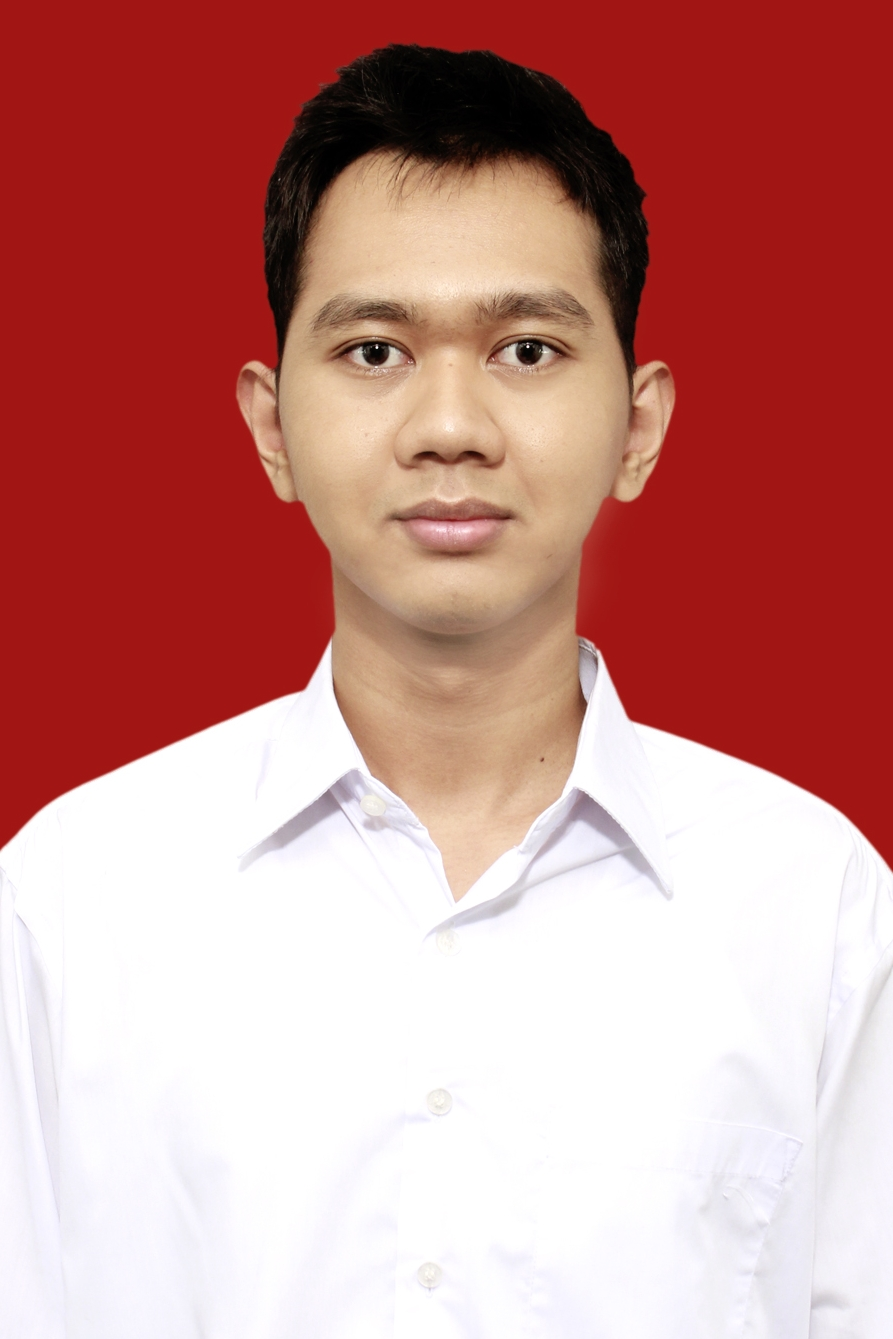
\includegraphics[scale=0.1]{pics/pengantar/BimaFoto.png}\hspace{4 cm}}
    & \kampus, \tanggalPengesahan \\
    & \\
    & \\
    & \penulis \\
    \cline{2-2}
    &  \nim\\
    \end{tabular}

% Abstrak Bahasa Indonesia dan Bahasa Iggris
\addChapter{ABSTRAK}

\chapter*{Abstrak}
\vspace*{0.7cm}

\noindent Abstrak ini\\



\vspace*{0.2cm}

\noindent Kata Kunci: \textit{kata kunci 1}, \textit{kata kunci 2}, \textit{kata kunci 3}, \textit{kata kunci 4}, \textit{kata kunci 5}\\ 

\newpage

\chapter*{ABSTRACT}
\vspace*{0.7cm}

\textit{Sensing Technology will become an important part of the future, one of its purposes is for object detection, velocity estimation, and ranging for speed trap camera on the side of the road to detect the velocity of vehicle so they wont surpass the chosen speed limit. Radar technology is one of sensing technology. Frequency Modulated Continuous Wave Radar is a popular technique that many people use. Many implementation of this technique is often use in various field, from automotive to health.}

\textit{In this research, a Software Defined Radio based FMCW radar has been design with GNURadio for detection, range estimation, and velocity of an object. The specification of system radar that has been designed is on 5.8 GHz carrier frequency, with a sawtooth modulation. The implementation use one unit of USRP with log periodic antenna. The result for range testing show a good quality from 6 meter above. The prediction accuracy for 6 meter is 82.86\% and the accuracy prediction for 9 meter is around 93.56\%. For range estimation at 3 meter, the prediction accuracy is at its worst, at about -402.72\%. The velocity experiment does not show a good quality}.

\noindent \textbf{Keywords}: \textit{FMCW}, \textit{Radar}, \textit{GNURadio}, \textit{USRP}, \textit{Detection}, \textit{Estimation}\\ 
\newpage

% Kata Pengantar
\addChapter{\kataPengantar}
%-----------------------------------------------------------------------------%
\chapter*{\kataPengantar}
%-----------------------------------------------------------------------------%
Kata Pengantar

\todo{tulis kata pengantar di sini}
 
\vspace*{0.1cm}
\begin{flushright}
Surabaya, \tanggalPengesahan\\[0.1cm]
\vspace*{1cm}
\penulis

\end{flushright}

%\addChapter{UCAPAN TERIMA KASIH}
%%-----------------------------------------------------------------------------%
\chapter*{Ucapan Terima Kasih}
%-----------------------------------------------------------------------------%
\todo{lalalal} 

\vspace*{0.1cm}
\begin{flushright}
Bandung, 1 April 2015\\[0.1cm]
\vspace*{1cm}
\penulis

\end{flushright}

% Daftar isi, gambar, dan tabel
\tableofcontents
\clearpage
\listoffigures
\clearpage
\listoftables
\clearpage
% Daftar Rumus
%\addChapter{DAFTAR RUMUS}
%%-----------------------------------------------------------------------------%
\chapter*{Daftar Rumus}
%-----------------------------------------------------------------------------%


% Daftar Lampiran
\addChapter{DAFTAR LAMPIRAN}
%-----------------------------------------------------------------------------%
\chapter*{Daftar Lampiran}
%-----------------------------------------------------------------------------%
\noindent
Lampiran A: Data Hasil Pengukuran\\
Lampiran B: Kode Program
\addChapter{DAFTAR ISTILAH}
%-----------------------------------------------------------------------------%
\chapter*{Daftar Istilah}
%-----------------------------------------------------------------------------%

\begin{tabular}{l c c c c l}
    Radar & & & & = & \textit{Radio Detection and Ranging} \\
    FMCW & & & & = & \textit{Frequency Modulated Continuous Wave} \\
    USRP & & & & = & \textit{Universal Software Radio Peripheral} \\
    SDR & & & & = & \textit{Software Defined Radio} \\
    LFM & & & & = & \textit{Linear Frequency Modulated} \\
    FFT & & & & = & \textit{Fast Fourier Transform} \\
    RMSE & & & & = & \textit{Root Mean Square Error} \\
    
\end{tabular}

% Gunakan penomeran Arab (1, 2, 3, ...) setelah bagian ini.
\pagenumbering{arabic}
% Bab 1 : Pendahuluan
%-----------------------------------------------------------------------------%
\chapter{\babSatu}
%-----------------------------------------------------------------------------%
%-----------------------------------------------------------------------------%
\section{Latar Belakang}
%-----------------------------------------------------------------------------%
Teknologi penginderaan sangat penting pada masa kini, salah satunya adalah untuk melakukan pendeteksian objek. Dalam implementasi pendeteksian objek, banyak cara yang dapat dilakukan agar hal itu bisa dicapai. Seperti contohnya adalah dengan menggunakan pengolahan visual dari hasil tangkapan kamera untuk melakukan analisis video, apalagi dengan menggunakan \textit{multi-camera network} \cite{Zhang2015}. Adapula penggunaan gelombang suara yang memanfaatkan frekuensi suara pada jarak ultrasonik untuk mendeteksi objek dan jarak dengan menggunakan mikrokontroler dan sensor ultrasonik \cite{Biswas2020}. Teknik lain yang menjadi alternatif adalah penggunaan gelombang elektromagnetik untuk mendeteksi objek dan jarak suatu benda dengan menggunakan radar. 

Radar adalah singkatan dari radio \textit{detection and ranging} yang berarti bahwa fokus kegunaan radar adalah pada pendeteksian dan estimasi jarak suatu benda dengan menggunakan gelombang elektromagnetik. Dibandingkan dengan teknik pengukuran lain, keunggulan dari penggunaan radar adalah mampu mendeteksi objek pada jarak yang jauh serta dapat menembus kabut. Keunggulannya tersebut adalah alasan awal digunakannya radar dahulu kala, yaitu  pada medan perang untuk mendeteksi pasukan sebelum nampak sehingga dapat melakukan persiapan terlebih dahulu. 

\begin{figure}
	\begin{center}
		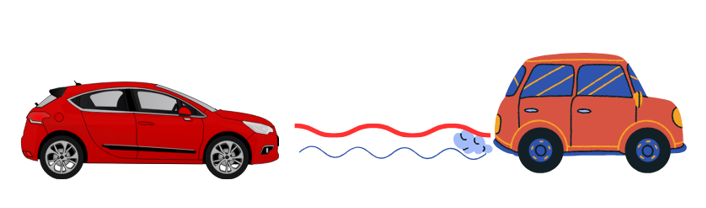
\includegraphics[scale=0.5]{pics/bab1/AplikasiRadar.png} 
		\caption[Penggunaan Radar Otomotif]{Penggunaan Radar Otomotif}
		\label{pic:aplikasiRadarKini}
	\end{center}
\end{figure}

Waktu berjalan dan zaman semakin modern serta peperangan mulai berkurang, maka radar pun beralih fungsi. Seperti contohnya radar pendeteksi cuaca yang digunakan oleh badan klimatologi untuk memudahkan prediksi cuaca, radar pada menara pengawas bandara yang berguna dalam memonitor pergerakan pesawat di udara, dan radar pendeteksi objek pada kendaraan otomotif yang berguna untuk mendeteksi objek dan mencegah tabrakan seperti pada gambar \ref{pic:aplikasiRadarKini}.

Kemampuan radar dalam melakukan deteksi dan estimasi jarak sangatlah penting, maka riset untuk mengembangkan implementasi radar dengan berbagai teknik semakin banyak \cite{Jia2020,Xia2021,MoraHuaman2020,Sundaresan2015}. Salah satu diantaranya adalah implementasi \textit{Real-Time Frequency Modulated Continuous Wave Radar} yang dikembangkan dengan GNURadio dan digunakan pada \textit{Software Defined Radio} \cite{Sundaresan2015}. Teknik \textit{Frequency Modulated Continuous Wave} atau yang disingkat dengan FMCW merupakan teknik transmisi secara kontinyu dari radar yang dapat memiliki energi yang lebih tinggi dengan \textit{peak power} yang lebih rendah \cite{Stasiak2017}. FMCW sangat populer digunakan pada industri, seperti untuk mendeteksi objek bawah tanah \cite{Macasero2018}, pada sistem pengawasan maritim \cite{Lestari2017}, dan bidang otomotif  karena dapat bertahan pada berbagai cuaca, dapat menghasilkan performa yang sangat baik, dapat memprediksi jarak dan kecepatan suatu objek \cite{Deng2017}. 

\textit{Software Defined Radio}, atau dalam kasus ini Radar, merupakan penggunaan fungsionalitas dari sistem radar yang diatur lewat \textit{Software} dengan maksud untuk memvirtualisasikan \textit{hardware} dan membuat manajemen pemrograman yang dilakukan menjadi lebih mudah \cite{Zeng2019}. Dengan menggunakan SDR lewat \textit{Universal Software Radio Peripheral} (USRP) sebagai perangkat kerasnya, maka proses riset dan pengembangan menjadi lebih murah, dikarenakan tidak diperlukannya fabrikasi material tiap uji coba pada frekuensi tertentu. Peneliti hanya perlu memprogram USRP yang dimilikinya untuk menghasilkan frekuensi tertentu yang mereka inginkan. Salah satu alat yang dapat digunakan dalam melakukan pemrograman terhadap USRP adalah GNURadio.


GNURadio merupakan aplikasi tak berbayar yang berada dibawah lisensi \textit{GNU General Public License} untuk mempelajari pembuatan dan pengimplementasian sistem \textit{software defined radio}. Dengan melakukan pemrograman pada GNURadio untuk melakukan antarmuka dengan USRP yang dimiliki, peneliti dapat menentukan berapa frekuensi hingga \textit{sampling rate} yang diinginkan \cite{Prabaswara2011}.

Oleh karena itu, pada proposal ini dilakukan “\judul” sehingga dapat membuktikan bahwa sistem yang dirancang dapat melakukan pendeteksian objek dan estimasi jarak.

%-----------------------------------------------------------------------------%
\section{Rumusan Masalah}
%-----------------------------------------------------------------------------%
Dari latar belakang yang telah dipaparkan diatas, maka ditemukannya rumusan masalah, yaitu:\\
\todo{Cek Ulang !!}
\begin{enumerate}
	\item Belum ada rancangan sistem radar FMCW menggunakan GNURadio yang memaksimalkan kemampuan USRP B210.
	\item Penggunaan GNURadio berbasis USRP 
	\item Bagaimana sistem radar FMCW berbasis USRP B210 yang telah dirancang dapat mendeteksi, mengestimasi jarak, dan kecepatan objek?
	\item Bagaimana tingkat keakurasian dari sistem radar FMCW pada USRP dalam mendeteksi, melakukan estimasi jarak, dan kecepatan objek?
\end{enumerate} 

%-----------------------------------------------------------------------------%
\section{Tujuan dan Manfaat}
%-----------------------------------------------------------------------------%
Dari rumusan masalah yang sudah didapatkan, maka bisa diambil beberapa tujuan yang ingin dicapai oleh penulis, yaitu:\\
\todo{Ubah !!}

\begin{enumerate}
	\item Untuk melakukan perancangan sistem radar FMCW berbasis USRP B210 menggunakan GNURadio.
	\item Untuk melakukan pengujian deteksi, estimasi jarak, dan kecepatan objek dari sistem radar FMCW pada USRP B210.
	\item Untuk mengetahui tingkat keakurasian pendeteksi, estimasi jarak, dan kecepatan objek menggunakan radar FMCW pada USRP.
\end{enumerate}

%-----------------------------------------------------------------------------%
\section{Batasan Masalah}
%-----------------------------------------------------------------------------%
Hal yang akan dilakukan dalam penelitian ini adalah.
\begin{enumerate}
	\item Parameter yang diidentifikasi pada rancang bangun ini adalah resolusi jarak, tingkat keakurasian, dan kecepatan.
	\item Pengujian sistem dengan menggunakan USRP B210 untuk melakukan pendeteksian, estimasi jarak, dan kecepatan objek.
	\item Perangkat lunak yang digunakan adalah GNURadio.
	\item Antena yang digunakan adalah antena \textit{Log Periodik}
	\item Frekuensi kerja radar pada 3 GHz.
	\item Objek deteksi adalah kendaraan empat roda.
\end{enumerate}

%-----------------------------------------------------------------------------%
\section{Metode Penelitian}
%-----------------------------------------------------------------------------%
Dalam melakukan pengerjaan Tugas Akhir yang diajukan, penyelesaian yang digunakan adalah dengan beberapa pendekatan yaitu: studi literatur, simulasi, analisis statistik, perancangan, dan implementasi.

%-----------------------------------------------------------------------------%
\section{Jadwal Penelitian}
%-----------------------------------------------------------------------------%
Untuk memastikan proposal ini berjalan dengan lancar, maka diperlukannya penentuan capaian yang ingin diraih pada suatu periode yang sudah ditentukan. Dengan teraihnya capaian tersebut maka tahapan selanjutnya dapat mulai dilakukan.

\begin{center}
	\begin{longtable}{|c|m{3.8cm}|c | m{3cm} |m{3cm}|}
		\caption{Agenda Penelitian}
		\label{tab:Agenda}\\
		\hline
		No. & Deskripsi Tahapan & Durasi & Tanggal & \textit{Milestone} \\
		\hline
		1. & Desain Sistem & 1 bulan & 1 September 2024 - 30 September 2024 & Diagram blok dan simulasi \\
		\hline
		2. & Implementasi dan pengujian& 1 bulan & 1 Oktober 2024 - 31 Oktober 2024 & Pengujian sistem selesai \\
		\hline
		3. & Penyusunan laporan Tugas Akhir & 2 minggu & 1 November 2024 - 15 November 2024 & Buku Tugas Akhir selesai \\
		\hline
	\end{longtable}
\end{center}


% Bab 2 : Landasan Teori
%-----------------------------------------------------------------------------%
\chapter{\babDua}
%-----------------------------------------------------------------------------%

%-----------------------------------------------------------------------------%
\section{Kajian Penelitian Terkait}
%-----------------------------------------------------------------------------%
Banyak sekali referensi yang menjadi bagian besar dalam tertulisnya proposal ini, referensi tersebut terdiri atas berbagai macam jenis literatur dari sumber yang dapat diakses secara daring. Tak sedikit pula literatur tersebut menjadi alasan besar latar belakang dari proposal ini dilahirkan, berikut adalah beberapa penelitian terdahulu yang menjadi referensi dalam melakukan penyusunan proposal ini :

% Penelitian Terdahulu
\begin{center}
	\newcolumntype{L}[1]{>{\raggedright\let\newline\\\arraybackslash\hspace{1pt}}m{#1}}
	\newcolumntype{C}[1]{>{\centering\let\newline\\\arraybackslash\hspace{1pt}}m{#1}}
	\newcolumntype{R}[1]{>{\raggedleft\let\newline\\\arraybackslash\hspace{1pt}}m{#1}}
	
	\begin{longtable}{|>{\centering\arraybackslash}p{0.6cm}|p{4cm}|p{4cm}|p{4cm}|}
	\caption{Penelitian Terdahulu}
	\label{tab:PenelitianDulu}\\
	\hline
	\textbf{No.} & \textbf{Judul} & \textbf{Penulis} & \textbf{Hasil}\\
	\hline
	1.& \textit{Respiratory and Heart Rate Detection Using Continuous-Wave Radar Testbed Implemented in GNU Radio } (2022)
	& Lenz, Isabella;\newline Holtom, Jacob;\newline Herschfelt, Andrew;\newline Rong, Yu;\newline Bliss, Daniel 
	& Penggunaan radar CW untuk memonitor detak jantung dan pernapasan menggunakan GNURadio dan USRP X310. Proses pengolahan data secara langsung dapat dilakukan dengan hasil estimasi di dalam jarak 5 BPM dibanding dengan alat monitor detak jantung. \\ \hline
	
	2. & \textit{Development of L-Band FMCW Radar on SDR using GNU RADIO} (2024)
	& Wankhede, Animesh;\newline De, Sampurna
	& Penggunaan radar FMCW pada pita frekuensi kelas L yang di aplikasikan sebagai radar penembus tanah menunjukkan hasil yang efektif dalam melakukan deteksi dan \textit{imaging} objek dengan akurasi dan resolusi tinggi.  \\ \hline
	
	3. & \textit{FMCW Radar With Enhanced Resolution and Processing Time by Beam Switching} (2021)
	& Hilario Re, Pascual D.;\newline Comite, Davide;\newline Podilchak, Symon K.;\newline Alistarh, Cristian A.;\newline Goussetis, George;\newline Sellathurai, Mathini;\newline Thompson, John;\newline Lee, Jaesup
	& Pengimplementasian radar FMCW pada pita frekuensi kelas K dengan antena \textit{array} dan \textit{beammforming} untuk sistem deteksi arah pada kendaraan otomotif. Dengan penggunaan frekuensi 24 GHz, radar mampu mendeteksi objek dengan jarak 2\textdegree.\\ \hline
	
	4. & \textit{An X–band FMCW Radar Demonstrator Based on an SDR Platform} (2020)
	& Dabrowski, Grzegorz;\newline Stasiak, Krzysztof;\newline Drozdowicz, Jedrzej;\newline Gromek, Damian;\newline Samczynski, Piotr
	& Desain dan implementasi radar FMCW dengan \textit{bandwidth} 1 GHz untuk mendapatkan resolusi jarak yang kecil dilakukan, didapati hasil pengujian yang memuaskan dengan menunjukkan adanya pergerakan pada daerah yang ditandai memiliki banyak aktivitas. \\ \hline
	
	5. & \textit{Single Target Recognition Using a Low-Cost FMCW Radar Based on Spectrum Analysis} (2020)
	& Rizik, Ali;\newline Tavanti, Emanuele;\newline Vio, Roberto;\newline Delucchi, Alessandro;\newline Chible, Hussien;\newline Randazzo, Andrea;\newline Caviglia, Daniele D.
	& Implementasi dan pengolahan sinyal radar dilakukan dengan melakukan klasifikasi terhadap data yang diterima. Klasifikasi dilakukan dengan menggunakan \textit{Support Vector Machine} (SVM), didapati hasil menunjukkan hasil akurasi klasifikasi target mencapai 100\%. \\ \hline
	
	6. & \textit{Educational Low-Cost C-Band FMCW Radar System Comprising Commercial Off-the-Shelf Components for Indoor Through-Wall Object Detection} (2021)
	& Jeong, Hyunmin;\newline Kim, Sangkil
	& Desain dan implementasi radar FMCW pada frekuensi kelas C dilakukan menggunakan komponen elektronik yang mudah didapat di pasar. Implementasi dilakukan dengan skenario pengujian dalam ruangan dan tembus dinding. Didapatkan hasil rata rata akurasi sekitar 5.6 cm dibanding data asli. \\ \hline
	
	7. & \textit{Modified FMCW system for non-contact sensing of human respiration} (2020)
	& Pramudita, Aloysius Adya;\newline Suratman, Fiky Y.;\newline Arseno, Dharu
	& Dengan melakukan modifikasi pada pendeteksian aktivitas pernafasan lewat pergeseran kecil, khususnya pada pengolahan data fasa setelah filter \textit{Low Pass}. Didapatkan hasil bahwa desain modifikasi mampu mendeteksi waktu dan amplitudo pernafasan, serta lokasi dari target. \\ \hline
	
	8. & \textit{FMCW Radar for Noncontact Bridge Structure Displacement Estimation} (2023)
	& Pramudita, Aloysius Adya;\newline Lin, Ding-Bing;\newline Dhiyani, Azizka Ayu;\newline Ryanu, Harfan Hian;\newline Adiprabowo, Tjahjo;\newline Yudha, Erfansyah Ali
	& Dilakukan implementasi radar FMCW pada frekuensi 24 GHz dengan \textit{bandwidth} 150 MHz untuk mendeteksi pergeseran kecil pada bangunan jembatan. Dengan menggunakan analisis fasa untuk mendapat resolusi yang baik dalam melakukan pendeteksian, didapat hasil bahwa metode berhasil dilakukan dengan kondisi banyak \textit{noise} dan nilai SNR rendah dengan rata rata galat 0.13 mm.\\ \hline
	
	9. & \textit{A Novel Scheme of High-Precision Heart Rate Detection With a mm-Wave FMCW Radar} (2023)
	& Zhou, Min;\newline Liu, Yunxue;\newline Wu, Shie;\newline Wang, Chengyou;\newline Chen, Zekun;\newline Li, Hongfei
	& Penggunaan radar FMCW dengan gelombang milimeter untuk monitor detak jantung telah banyak dilakukan. Sehingga usaha peningkatan akurasi menjadi arah selanjutnya, dengan implementasi algoritma \textit{Variable Mode Extraction} sinyal detak jantung di ambil dan teknik pengukuran frekuensi \textit{Double-CZT} dilakukan. Hasil menunjukkan tingkat akurasi yang meningkat dengan rata rata eror absolut kurang dari 1 bpm, selain itu nilai SNR meningkat sehingga estimasi akurasi detak jantung juga meningkat.\\ \hline
	\end{longtable}
\end{center}
%-----------------------------------------------------------------------------%
%\section{Teori Dasar}
%-----------------------------------------------------------------------------%

\section{Radar}

Penggunaan gelombang elektromagnetik sebagai sarana untuk mendeteksi objek adalah konsep dasar dari radar. Radar sendiri merupakan singkatan dari \textit{Radio Detection and Ranging}, dari situ sangat nampak sekali tujuan dari penggunaan alat ini, yaitu untuk mendeteksi sesuatu dan mengukur jarak dengan menggunakan gelombang radio. 

Cara kerja dari radar adalah dengan memancarkan gelombang di dalam ruang bebas yang kemudian radar akan mendeteksi gelombang pantulan dari objek tersebut. Adanya gelombang yang terpantul ini tidak hanya menunjukkan keberadaan dari suatu objek, namun dengan membandingkan gelombang pantulan yang diterima dengan gelombang yang dikirimkan maka informasi tentang objek yang terdeteksi dapat didapat \cite{Skolnik2001}.

\begin{equation}
	R = \frac{cT_{R}}{2}
	\label{eq:PersRadar}
\end{equation}

Persamaan \ref{eq:PersRadar} menjelaskan jarak antara target dengan antena, dengan $T_{R}$ sebagai waktu sinyal radar bergerak secara bolak balik dari dan menuju objek. Karena radar memakai gelombang elektromagnetik, maka $c$ memiliki kecepatan yang sama dengan cahaya, yaitu $3 \times 10 ^{8}$.

Pada gambar \ref{pic:skemaRadar} berikut, skema dan konsep dasar dari cara kerja radar dapat diamati. Terlihat bahwa sinyal yang dikirimkan akan mengenai target, dalam kasus ini adalah pesawat, lalu sinyal yang mengenai objek akan kembali dengan sinyal yang lebih kecil dengan amplitudo yang lebih rendah. Perubahan pada gelombang yang terpantul dapat menggambarkan perilaku yang sedang ditunjukkan oleh objek yang di deteksi, mulai dari pengurangan amplitudo hingga pergeseran fasa.

\begin{figure}
	\begin{center}
		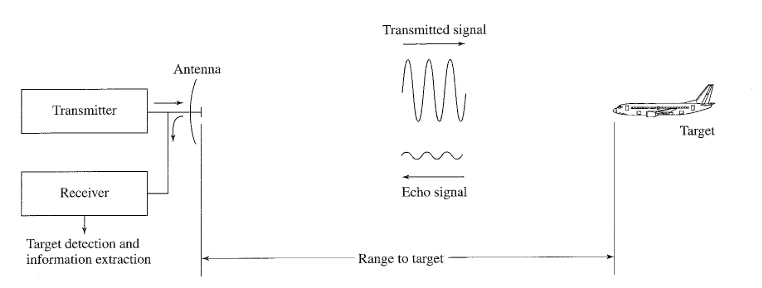
\includegraphics[scale=0.5]{pics/bab2/skemaradar.png} 
		\caption[Skema Dasar Radar]{{Skema Dasar Radar} \cite{Skolnik2001}}
		\label{pic:skemaRadar}
	\end{center}
\end{figure}

Gambar \ref{pic:blokdiagram} menunjukkan blok diagram dari sistem radar pulsa sederhana. Dapat dilihat beberapa komponen yang membentuk seluruh sistem radar, semua komponen ini memiliki perannya sendiri sehingga proses pengiriman dan pendeteksian sinyal dapat dilakukan.  Bila seluruh sistem bekerja dengan baik, maka proses yang ditunjukkan pada penjelasan skema dasar radar dapat berjalan dengan lancar.

\begin{figure}
	\begin{center}
		\includegraphics[scale=0.35]{pics/bab2/blokdiagram.png} 
		\caption[Blok Diagram Radar]{{Blok Diagram Radar Sederhana \cite{Kingsley1999}}}
		\label{pic:blokdiagram}
	\end{center}
\end{figure}

Persamaan radar berguna untuk menghubungkan seluruh komponen yang terdapat pada suatu sistem radar. Hubungan di antara seluruh komponen tersebut akan di perlihatkan secara matematis, sehingga penerapannya pada suatu alat akan terlihat dengan jelas. Dengan adanya beberapa persamaan ini, proses desain suatu radar akan menjadi lebih mudah dilakukan dan prediksi dari hasil radar yang dirancang bisa didapatkan.

Salah satu persamaan pada radar adalah \textit{maximum unambiguous range}, yang bersimbol $R_{un}$, dengan $T_{p}$ sebagai periode pengulangan pulsa, yang bernilai $\frac{1}{f_{p}}$, dengan $f_{p}$ sebagai frekuensi pengulangan pulsa.

\begin{equation}
	R_{un} = \frac{cT_{p}}{2} = \frac{c}{2f_{p}}
\end{equation}

Bila antena yang digunakan dalam memancarkan gelombang elektromagnetika radar bersifat isotrop, maka kerapatan daya pada jarak $R$ dari radar akan sama dengan daya di transmisi ($P_{t}$) dibagi luas permukaan $4\pi R^{2}$ dari sebuah bola imajiner dengan radius $R$, atau dapat didefinisikan pula dengan.

\begin{equation}
	P = \frac{P_{t}}{4\pi R^{2}}
\end{equation}

Namun, pada kenyataannya radar seringkali menggunakan antena \textit{directive} untuk mengkonsentrasikan daya yang terradiasi pada arah tertentu. Maka kerapatan dayanya adalah

\begin{equation}
	\text{Kerapatan daya antena \textit{directional}} = \frac{P_{t} G}{4\pi R^{2}}
\end{equation}

Dengan G sebagai \textit{gain} maksimum suatu antena, yaitu

\begin{equation}
	G  = \frac{\text{Kerapatan daya maksimum dari antena \textit{directional}}}{\text{Kerapatan daya antena Isotrop \textit{lossless} dengan daya yang sama}}
\end{equation}

\textit{Radar Cross Section} atau yang sering disingkat dengan RCS merupakan daerah suatu objek dari target yang dapat terdeteksi oleh suatu radar. Area tersebut diperhitungkan dengan mempertimbangkan bentuk dari objek dan interaksinya dengan gelombang elektromagnetik. Pada \ref{pic:RCS} ditunjukkan beberapa sifat RCS dan persamaannya.

\begin{center}
	\begin{figure}[h!]
		\begin{subfigure}[b]{0.5\linewidth}
			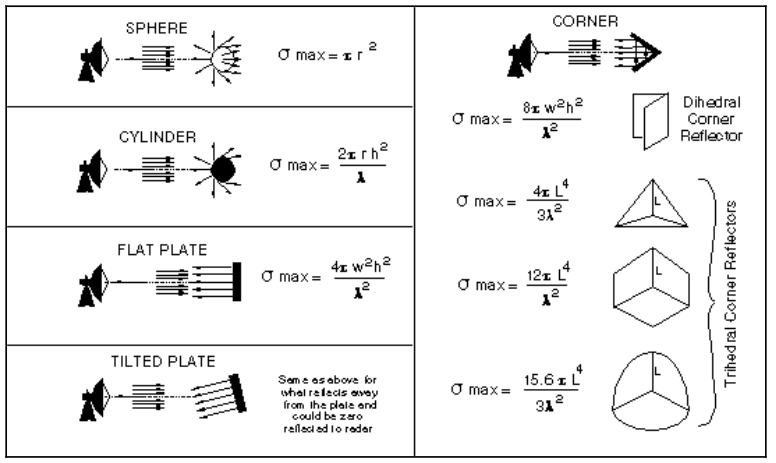
\includegraphics[width=\linewidth]{pics/bab2/rcsBentuk.png}
			\caption{Bentuk dan Persamaan \textit{Radar Cross Section}}
		\end{subfigure}
		\begin{subfigure}[b]{0.5\linewidth}
			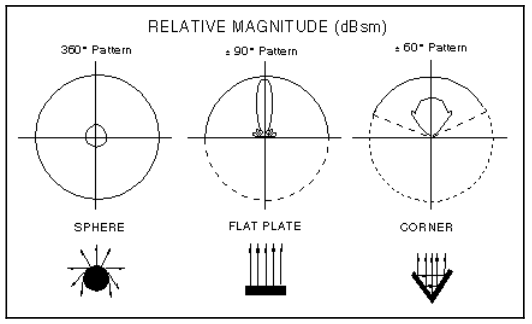
\includegraphics[width=\linewidth]{pics/bab2/rcsPola.png}
			\caption{Pola Radiasi dari \textit{Radar Cross Section}}
		\end{subfigure}
		\caption[\textit{Radar Cross Section}]{\textit{Radar Cross Section} \cite{ONeill2012}}
		\label{pic:RCS}
	\end{figure}
\end{center}

\section{Pengolahan Sinyal Radar}
Untuk mendapat suatu kesimpulan dari sinyal radar, maka dibutuhkan pengolahan sinyal radar yang tepat. Pengolahan sinyal tersebut dilakukan mulai dari pembentukan gelombang hingga pengambilan kesimpulan. 

\subsection{Bentuk Gelombang Radar}
\begin{figure}
	\begin{center}
		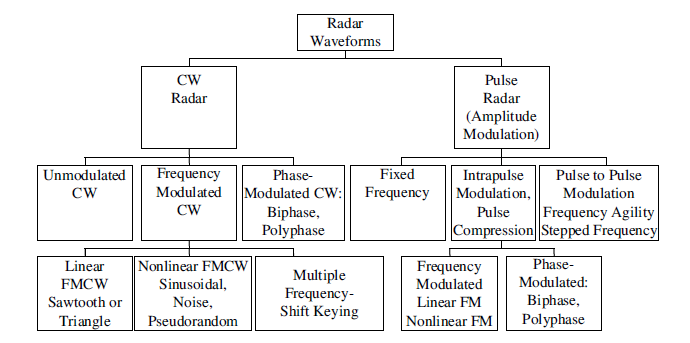
\includegraphics[scale=0.8]{pics/bab2/radarwaveform.png}
		\caption[Bentuk Gelombang Radar]{Bentuk Gelombang Radar \cite{Melvin2014}}
		\label{pic:bentukgelradar}
	\end{center}
\end{figure}
Bentuk gelombang radar dapat dibedakan menjadi dua kelas, yaitu radar dengan gelombang kontinyu dan radar pulsa. Seperti pada gambar \ref{pic:bentukgelradar}, kedua kelas tersebut masih dapat dibagi lagi kedalam beberapa teknik lain. Penggunaan salah satu jenis gelombang ditentukan berdasarkan kebutuhan radar yang akan di desain. 

Radar dengan gelombang pulsa akan memancarkan gelombang elektromagnetik dalam waktu singkat lalu jeda sejenak sesuai waktu yang ditentukan. Pada waktu jeda tersebut, radar akan mendeteksi sinyal pantul dari gelombang yang dikirim sebelumnya. Setelah waktu jeda berakhir, radar akan kembali memancarkan gelombang pulsa lagi. Radar dengan gelombang ini akan memancarkan gelombang elektromagnetik dengan \textit{power} yang tinggi. 

Sedangkan radar dengan gelombang kontinyu akan terus memancarkan serta menerima gelombang elektromagnetik tanpa henti dalam waktu yang bersamaan. Sehingga radar dengan gelombang kontinyu hanya digunakan pada sistem dengan \textit{power} yang rendah dengan jarak maksimum deteksi yang kecil. Hal ini disebabkan karena sering terjadinya kebocoran dari antena pengirim ke antena penerima. Alasan ini pula yang mendasari keputusan penggunaan \textit{power} yang rendah \cite{Scheer2015}.

\subsection{\textit{Frequency Modulated Continuous Wave Radar}}

Radar FMCW memancarkan sinyal yang bila terpantul objek, akan kembali terdeteksi. Hal ini dapat direalisasikan dengan blok diragram dari sistem radar FMCW seperti pada gambar \ref{pic:FMCWBlock}.  

\begin{figure}
	\begin{center}
		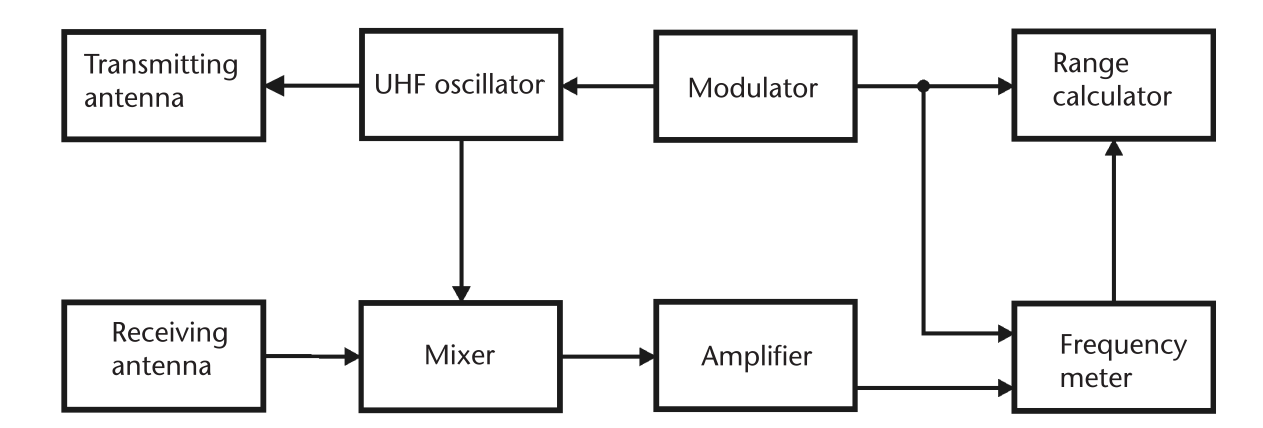
\includegraphics[scale=0.3]{pics/bab2/blokDiagramFMCW.png}
		\caption[Blok Diagram Radar FMCW]{Blok Diagram Radar FMCW}
		\label{pic:FMCWBlock}
	\end{center}
\end{figure}

Dari blok diagram tersebut, dapat dilihat bahwa sinyal yang diterima dicampurkan dengan sinyal yang dikirim, sehingga karena adanya \textit{delay} yang disebabkan oleh jarak gelombang bergerak, maka akan terdeteksi perbedaan frekuensi. Dengan begitu, perbedaan pada fasa dan frekuensi menjadi tolok ukur antara sinyal yang dikirim dengan sinyal yang di dapatkan kembali.

\begin{figure}
	\begin{center}
		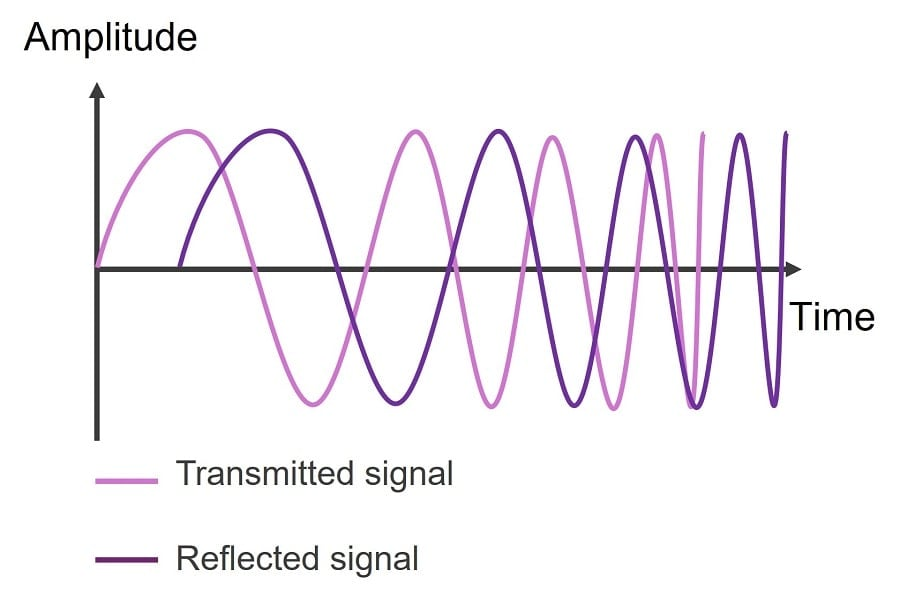
\includegraphics[scale=0.3]{pics/bab2/txRxWave.jpg}
		\caption[FMCW Dalam Domain Waktu]{FMCW Dalam Domain Waktu}
		\label{pic:FMCWTime}
	\end{center}
\end{figure}

Oleh karena itu, salah satu karakteristik dari radar FMCW adalah bahwa jarak pengukuran dapat dihitung dengan membandingkan frekuensi sinyal yang diterima dengan sinyal yang ditransmisikan.   

\begin{equation} 
	R = \frac{c \Delta{t}}{2} = \frac{c \Delta{f}}{2(\frac{d(f)}{d(t)})}
	\label{eq:PersFMCW}
\end{equation}

Persamaan \ref{eq:PersFMCW} menunjukkan jarak (R) dengan objek yang terdeteksi. Yang mana $\Delta{t}$ adalah waktu tunda dalam detik, $\Delta{f}$ merupakan pergeseran frekuensi terukur dalam Hertz, dengan d(f)/d(t) sebagai pergeseran frekuensi dalam suatu periode. 

\begin{equation}
	R_{max} = \frac{F_{s} c}{2 \mu}
	\label{eq:MaxRange}
\end{equation}

Persamaan \ref{eq:MaxRange} menunjukkan jarak maksimum yang dapat di deteksi oleh radar FMCW. $F_{s}$ merupakan frekuensi \textit{sampling}, dan $\mu$ adalah tingkat kenaikan frekuensi pada suatu periode yang dapat dihitung dengan persamaan \ref{eq:chirpRate} yaitu membagi nilai \textit{bandwidth} dengan waktu \textit{sweep} (\textit{chirp}) bersimbol $T_{c}$.

\begin{equation}
	\mu = \frac{\textit{Bandwidth}}{T_{c}}
	\label{eq:chirpRate}
\end{equation}

Dengan nilai $T_{c}$ sebagai berikut

\begin{equation}
	T_{c} = \frac{\lambda}{4 \cdot V_{max}}
	\label{eq:chirpTime}
\end{equation}

Selain itu, salah satu faktor penting yang perlu diperhitungkan dalam perancangan radar FMCW adalah resolusi jarak. Resolusi jarak sendiri merupakan kemampuan dari suatu radar dalam membedakan dua buah objek yang berdekatan.

\begin{equation}
	R_{res} = \frac{c}{2 BW}
	\label{eq:RangeRes}
\end{equation}

Persamaan \ref{eq:RangeRes} menjelaskan bahwa dengan membagi kecepatan cahaya dengan dua kali lebar pita frekuensi (\textit{Bandwidth}), maka resolusi jarak akan didapatkan. Sedangkan nilai kecepatan maksimum dapat dihitung dengan persamaan \ref{eq:maxVelo} yang melakukan pembagian panjang gelombang frekuensi dipilih dengan 4 dikali \textit{sweep time}.
\begin{equation}
	v_{max} = \frac{\lambda}{4 \cdot T_{c}}
	\label{eq:maxVelo}
\end{equation}

Sehingga nilai resolusi kecepatan dapat dihitung dengan persamaan \ref{eq:resVelo}, yang membagi panjang gelombang dengan 2 kali durasi \textit{frame} ($T_{f}$).

\begin{equation}
	V_{res} = \frac{\lambda}{2 \cdot T_{f}}
	\label{eq:resVelo}
\end{equation}

$T_{f}$ sendiri adalah durasi dari \textit{frame} yang terdiri dari N jumlah dari \textit{chirp} secara terus menerus, nilainya dapat dicari pada persamaan \ref{eq:frameDuration}.

\begin{equation}
	T_{f} = N \cdot T_{c} = \frac{\lambda}{2 \cdot V_{res}}
	\label{eq:frameDuration}
\end{equation}

\subsection{\textit{Linear Frequency Modulated Continuous Wave Radar}}
\textit{Linear Frequency Modulated}, yang juga sering disingkat sebagai LFM adalah teknik pengolahan sinyal yang dilakukan dengan menyapu frekuensi dari bawah ke atas (\textit{Up-Chirp}) atau dari atas ke bawah (\textit{Down-Chirp}). Dengan $f_{0}$ sebagai frekuensi tengah, dan dilakukan pada \textit{bandwidth} yang telah ditentukan. Teknik ini akan membantu pencapaian radar dengan resolusi yang lebih tinggi karena \textit{bandwidth} yang dicapai akan menjadi lebih tinggi.

Salah satu jenis gelombang LFM adalah \textit{Linear Triangular Frequency Modulation} yang ditunjukkan pada gambar \ref{pic:LFMTriangular}. Penggunaan jenis gelombang tersebut akan mempermudah proses evaluasi target.

\begin{figure}
	\begin{center}
		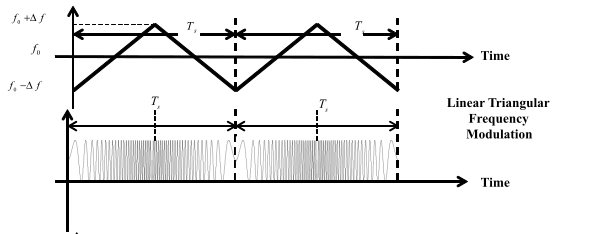
\includegraphics[scale=0.7]{pics/bab2/lfmTriangular.png}
		\caption[LFM Tipe Segitiga]{LFM Tipe Segitiga \cite{Jankiraman2018}}
		\label{pic:LFMTriangular}
	\end{center}
\end{figure}


Selain gelombang LFM segitiga, ada pula yang berbentuk seperti gigi gergaji (\textit{Sawtooth}) seperti gambar \ref{pic:lfmSaw}.

\begin{figure}
	\begin{center}
		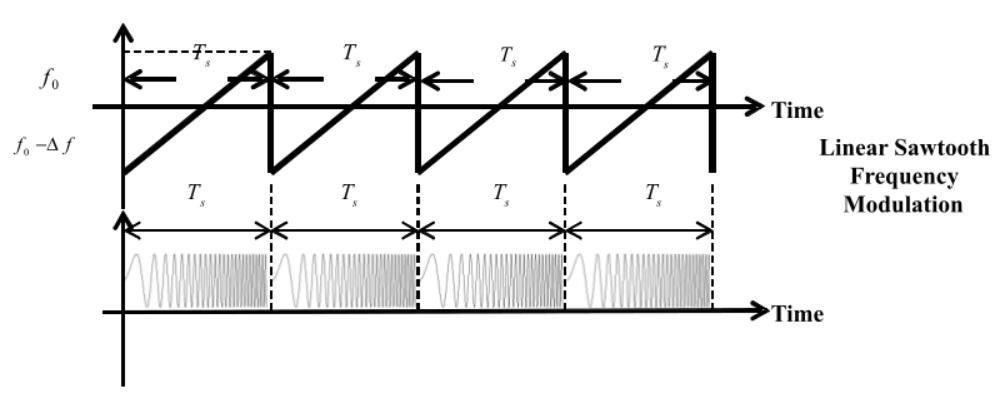
\includegraphics[scale=0.65]{pics/bab2/lfmSawtooth.png}
		\caption[LFM Tipe Gigi Gergaji]{LFM Tipe Gigi Gergaji \cite{Jankiraman2018}}
		\label{pic:lfmSaw}
	\end{center}
\end{figure}

Seluruh teknik tersebut memiliki keunggulannya masing-masing. Keunggulan tersebut didapat karena proses analisis yang berbeda. Pada LFM berbentuk gigi gergaji, maka hanya objek diam saja yang dapat dideteksi jarak dan kecepatannya seperti pada gambar \ref{pic:lfmDetail}. Namun bila menggunakan LFM berbentuk segitiga, maka objek yang bergerak dapat dideteksi jarak dan kecepatannya dalam waktu yang bersamaan.

\begin{figure}
	\begin{center}
		\includegraphics[scale=0.65]{pics/bab2/lfmDetail.png}
		\caption[Detail Analisis LFM \textit{Sawtooth}]{Detail Analisis LFM \textit{Sawtooth} \cite{Jankiraman2018}}
		\label{pic:lfmDetail}
	\end{center}
\end{figure}


\subsection{Teknik Pengolahan Sinyal}
Untuk melakukan pengambilan keputusan dari data yang diambil oleh radar, maka dibutuhkan langkah pengolahan yang benar dan mencakup berbagai hal. Beberapa parameter yang bisa diambil estimasinya adalah jarak dan kecepatan dari objek yang terdeteksi. Pada estimasi jarak, persamaan \ref{eq:RangeEst} dapat menjelaskan hubungan jarak dengan beberapa faktor yang mempengaruhinya.

\begin{equation}
	d_{0} = \frac{c f_{b}}{2 \mu} = \frac{c T_{c} f_{b}}{2 B}
	\label{eq:RangeEst}
\end{equation}

Pada persamaan tersebut, terdapat c sebagai kecepatan cahaya, $f_{b}$ adalah \textit{beat frequency} yang merupakan perbedaan pada frekuensi,  $\mu$ yang merupakan laju perubahan frekuensi pada suatu waktu (\textit{chirp rate}), dengan $T_{c}$ sebagai waktu \textit{Sweep}. Sedangkan untuk melakukan estimasi kecepatan terdapat pergeseran frekuensi akibat efek doppler, yang menjelaskan perubahan frekuensi suatu gelombang karena suatu objek sumber yang bergerak. Bila pergeseran doppler ($f_{d}$), dengan v sebagai kecepatan, dan $\lambda$ adalah panjang gelombang, maka didapatkan persamaan \ref{eq:velocity}.

\begin{equation}
	v = \frac{f_{d}}{2}\lambda
	\label{eq:velocity}
\end{equation}

\subsection{Perhitungan \textit{Error}}
Penghitungan galat dari radar yang telah di desain dapat dilakukan dengan menguji keakurasian dari hasil deteksi. Hasil akurasi deteksi radar dapat diuji dengan menggunakan \textit{Root Mean Square Error} (RMS E) dari \textit{Signal to Noise Ratio}, sesuai persamaan \ref{eq:sigmaRN}.

\begin{equation}
	\sigma_{RN} = \frac{RMS E}{\sqrt{2 SNR_{L}}}
	\label{eq:sigmaRN}
\end{equation}

Dengan nilai dari RMS E bisa didapat dengan persamaan \ref{eq:rmsE}.

\begin{equation}
	RMS E = \frac{\sqrt{\sum_{t = 1}^{k} (m(t)-n(t))^2}}{k}
	\label{eq:rmsE}
\end{equation}

Nilai dari k adalah jumlah data, dengan m sebagai hasil data berdasarkan simulasi, dan n adalah data sebenarnya. Dengan begitu, nilai akurasi deteksi radar dapat dihitung dengan persamaan \ref{eq:accRadar}.

\begin{equation}
	Akurasi = 1 - \sigma_{RN}
	\label{eq:accRadar}
\end{equation}

\section{\textit{Software Defined Radio}}
\textit{Software Defined Radio} atau yang sering disingkat menjadi SDR merupakan teknologi komunikasi berbasis nirkabel yang kegunaannya dapat ditentukan oleh perangkat lunak \cite{Anisah2018}. Sehingga dalam implementasinya, tidak perlu dilakukan perubahan perangkat keras baru bila ingin melakukan perubahan, baik dari segi standar, teknologi, dan layanan. Hanya dengan melakukan perubahan konfigurasi saja, lalu SDR akan langsung dapat digunakan. 

Dalam implementasinya, SDR membutuhkan \textit{Universal Software Radio Peripheral}, atau yang sering disingkat menjadi USRP merupakan \textit{hardware} yang merupakan bagian \textit{front end} pada arsitektur sistem SDR. USRP terdiri dari modul yang dapat terkoneksi dengan komputer sehingga memperbolehkan pemrograman dengan aplikasi seperti GNURadio dan LabVIEW \cite{Gulo2023}. 

Penggunaan USRP sangat memudahkan proses perancangan prototipe dan pengujian karena adanya antarmuka yang dapat mengkoneksikan USRP dengan antena dan berbagai macam bagian perangkat keras yang dibutuhkan.

\subsection{\textit{Universal Software Radio Peripheral}}

\textit{Universal Software Radio Peripheral} sering disingkat USRP merupakan \textit{platform} yang digunakan dalam mengimplementasikan SDR. Di dalam USRP terdapat \textit{Field Programmable Gate Array} atau FPGA yang merupakan suatu \textit{Integrated Circuit} yang dapat diprogram. Pada hal ini, USRP adalah perangkat keras yang dapat menerima dan mentransmisikan gelombang radio.

Kemampuannya untuk berinteraksi dengan gelombang radio inilah, ditambah dengan kemudahannya untuk melakukan pemrograman terhadap USRP yang membuat alat ini terkenal di kalangan akademisi dan peneliti. Karena pengembangan prototipe menjadi lebih mudah tanpa perlu pengadaan komponen.

\begin{center}
	\begin{figure}[h!]
		\begin{subfigure}[b]{0.5\linewidth}
			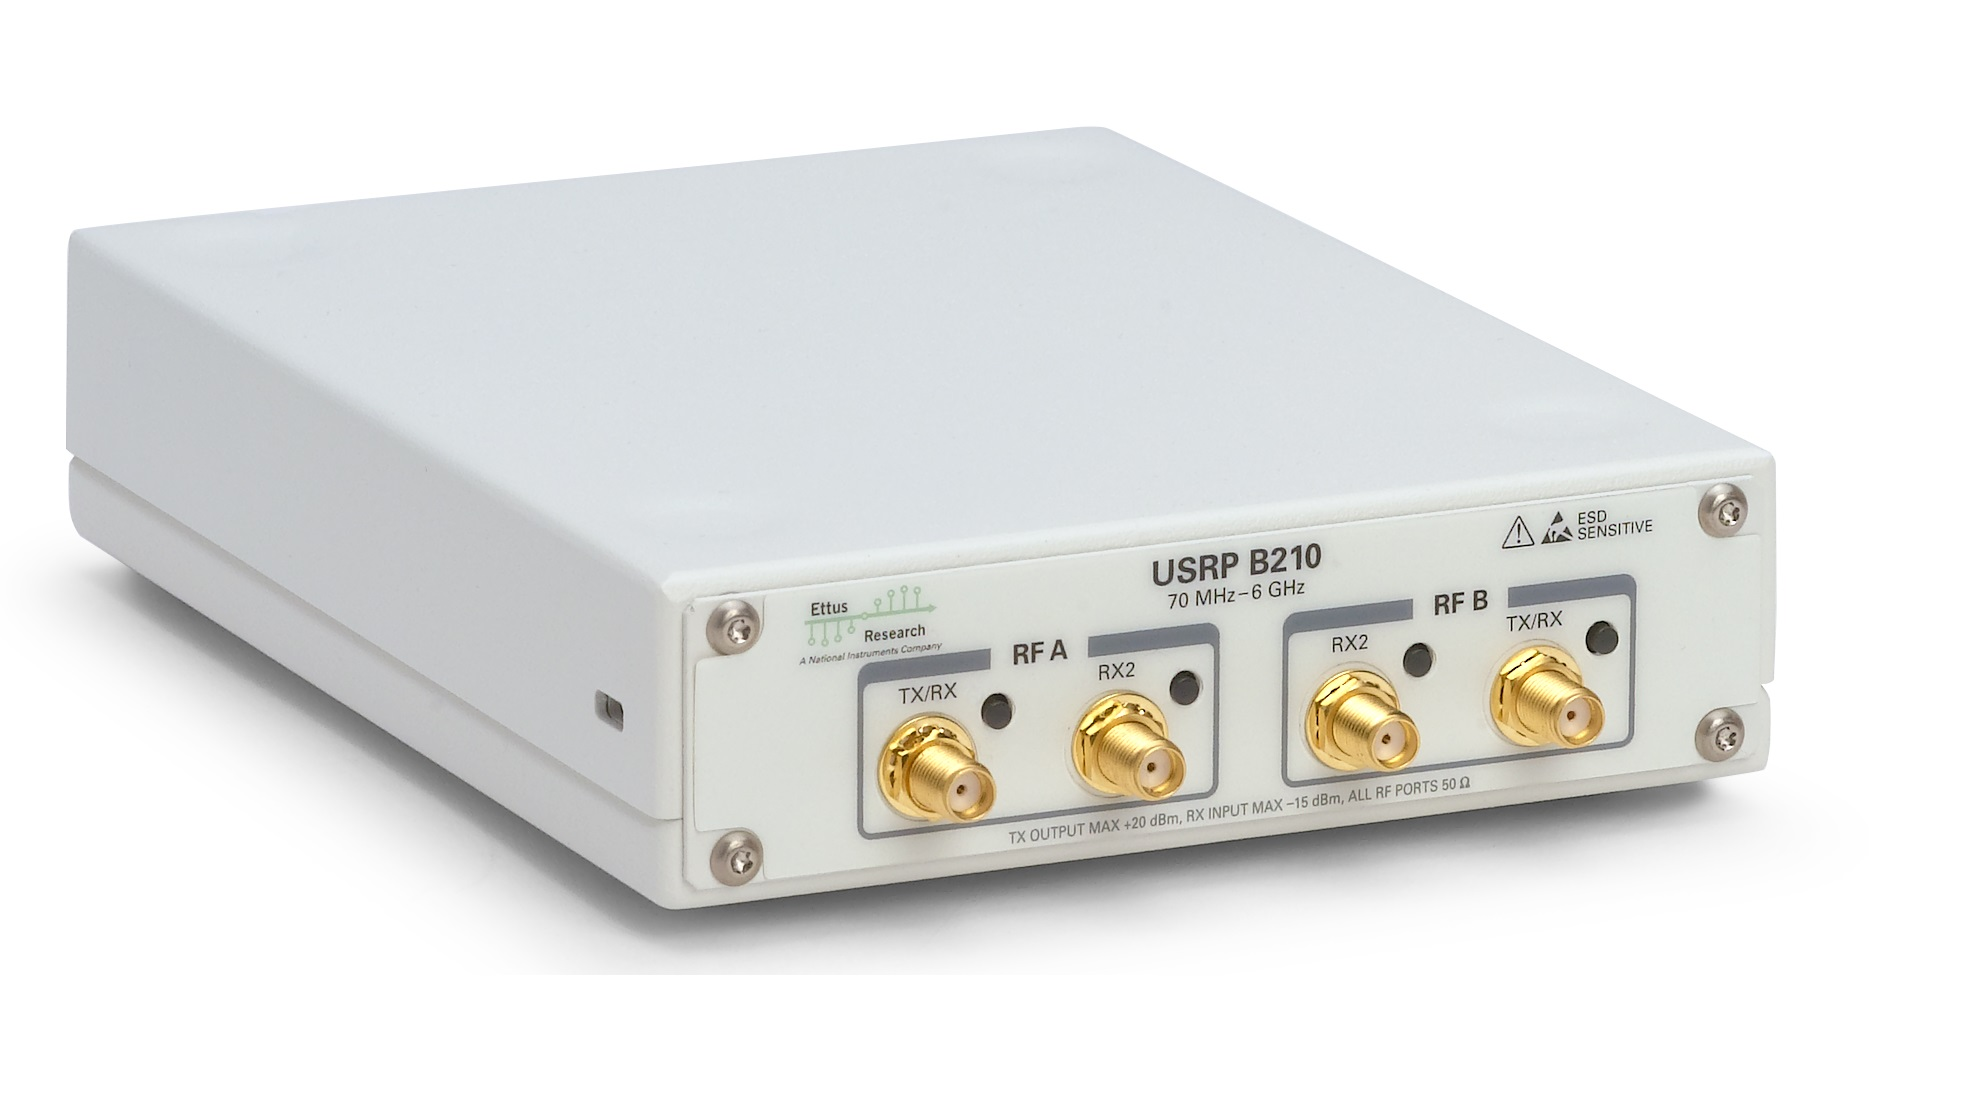
\includegraphics[width=\linewidth]{pics/bab2/B210.jpg}
			\caption{USRP B210 dengan \textit{enclosure}}
		\end{subfigure}
		\begin{subfigure}[b]{0.5\linewidth}
			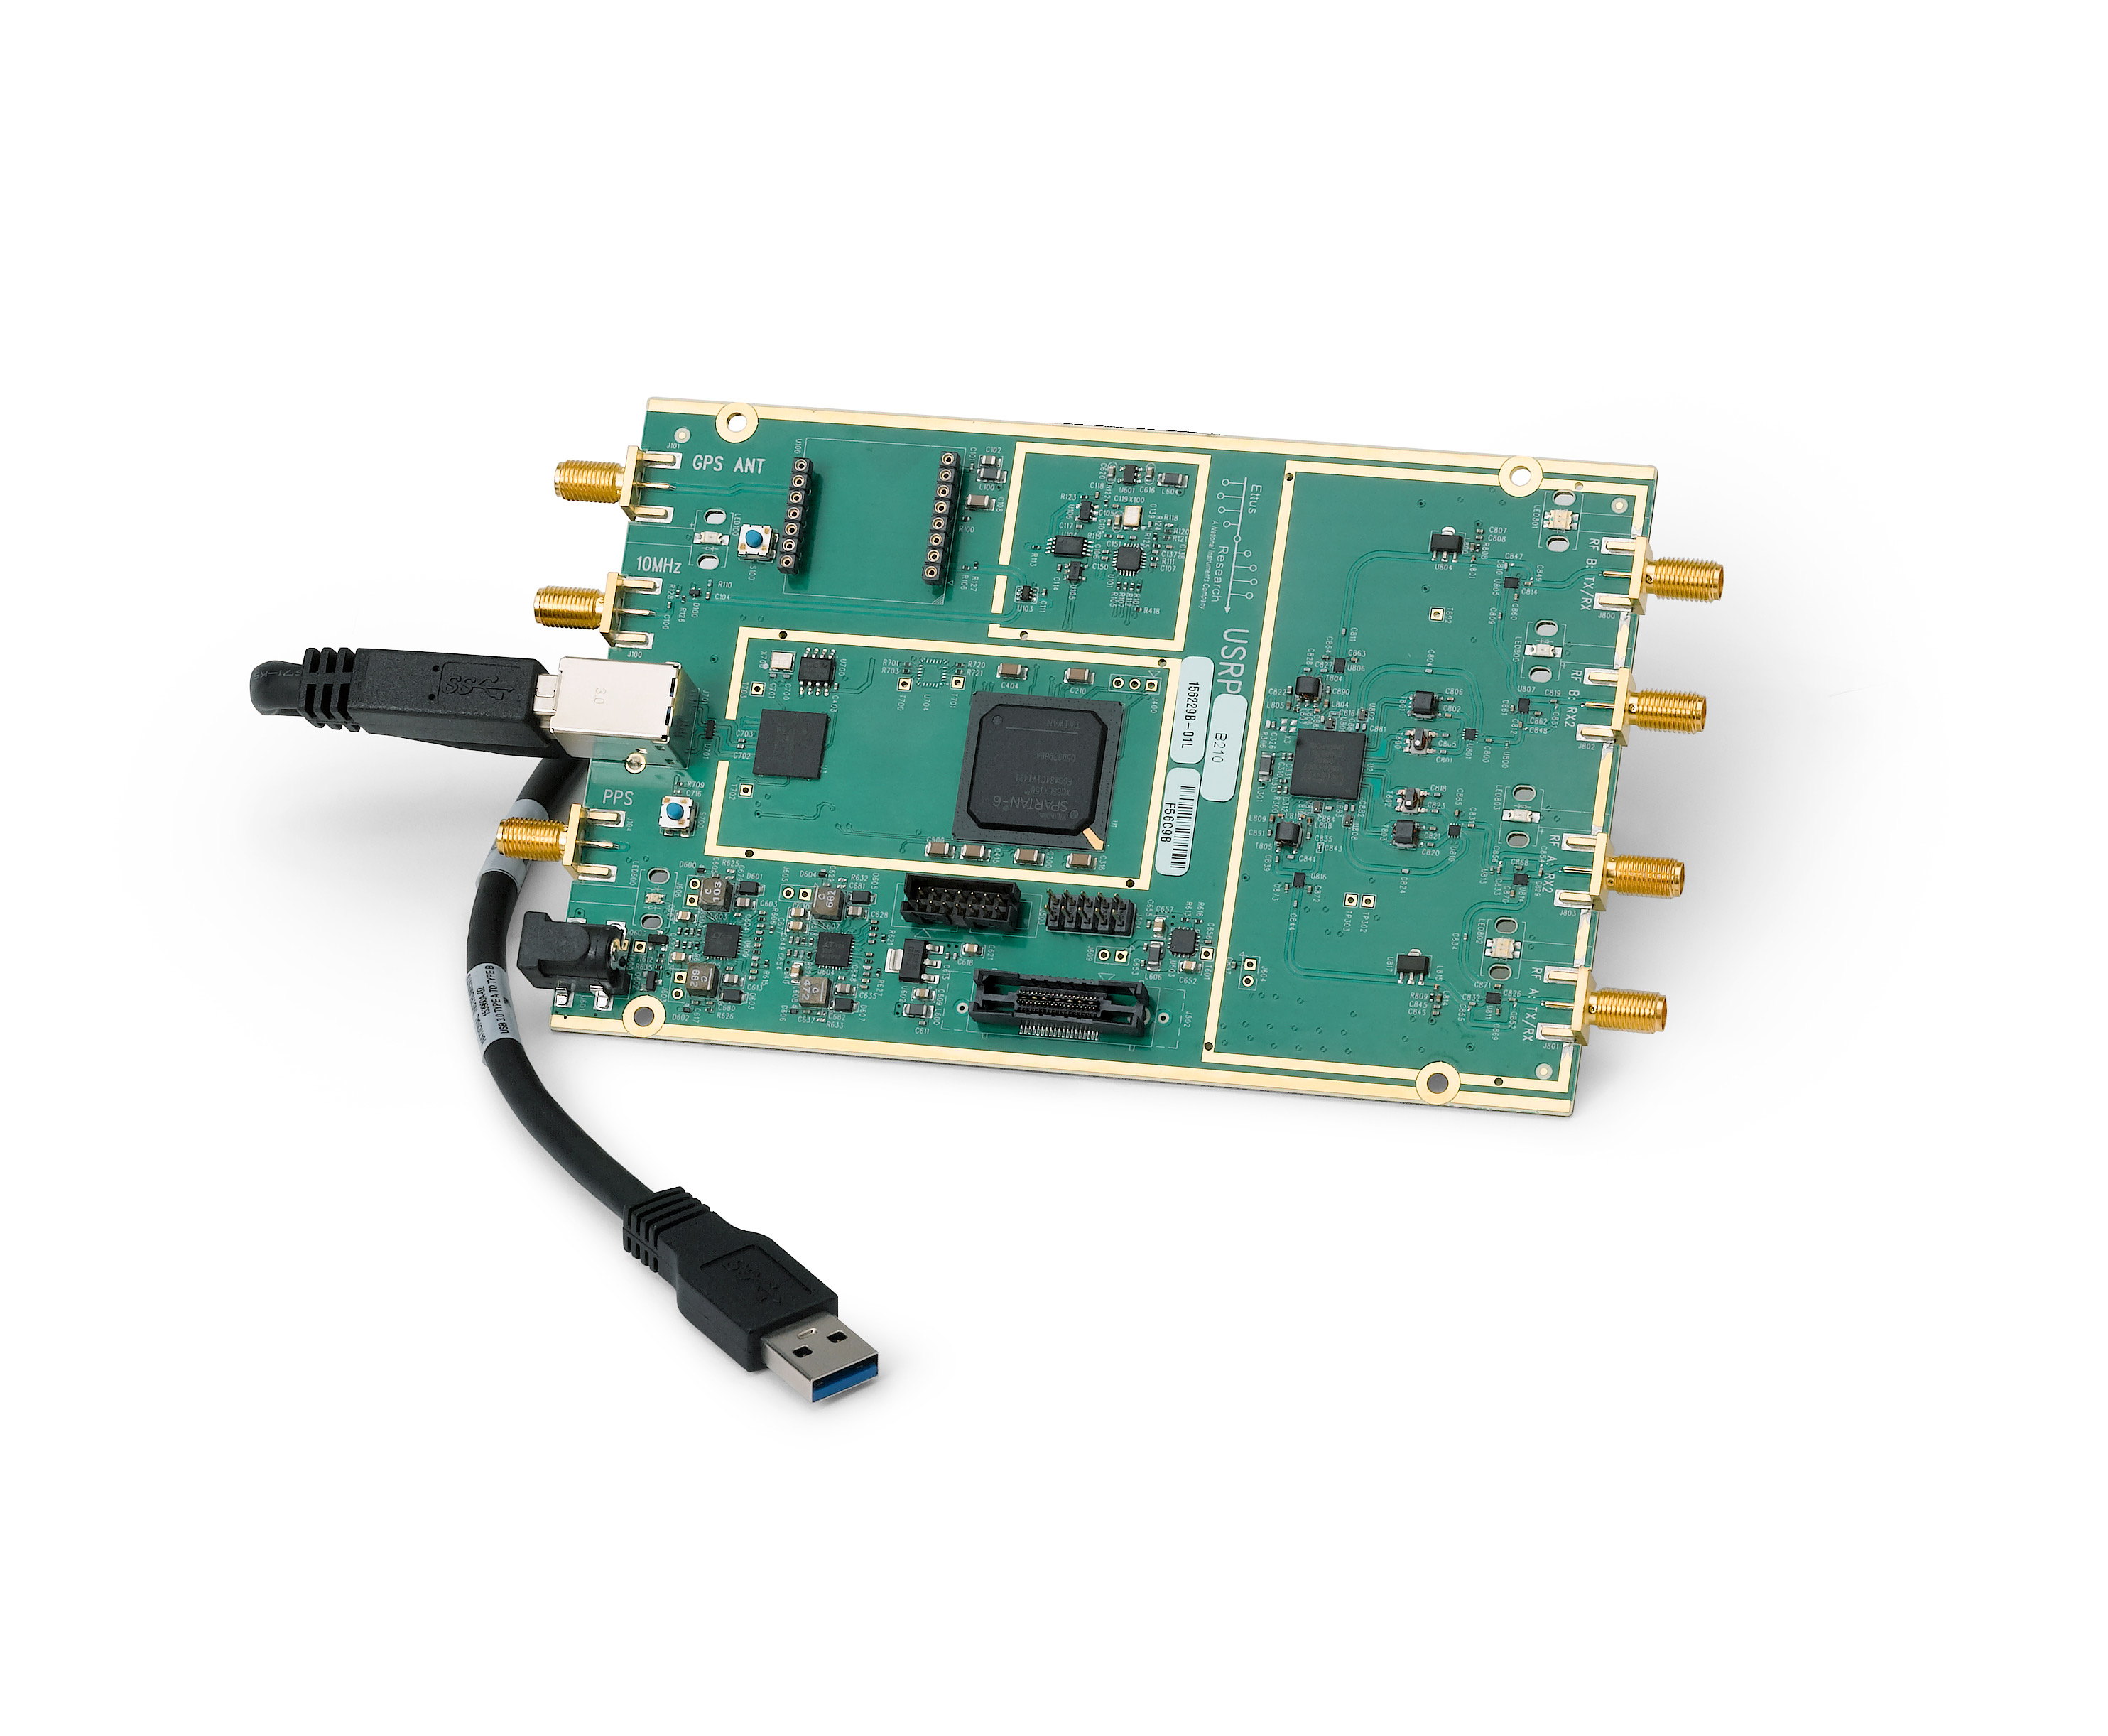
\includegraphics[width=\linewidth]{pics/bab2/B210Board.jpg}
			\caption{\textit{Board} USRP B210}
		\end{subfigure}
		\caption{USRP B210}
		\label{pic:gambarusrp}
	\end{figure}
\end{center}

Ada beberapa USRP di pasaran, salah satunya adalah USRP buatan dari \textit{Ettus} dengan seri B210 seperti pada gambar \ref{pic:gambarusrp}. Penggunaan seri ini dikarenakan seperti yang dapat dilihat pada tabel spesifikasi \ref{tab:spekb210}, USRP ini cukup memenuhi kebutuhan riset dengan kapabilitas pengolahan sampel yang baik.

\begin{longtable}{|c|c|c|c|}
	\caption{Spesifikasi \textit{USRP} B210}
	\label{tab:spekb210}\\
	\hline
	No. & Keterangan & Nilai & Satuan \\
	\hline
	1. & \textit{RF Coverage} & 70 - 6 & MHz - GHz \\
	\hline
	2. & \textit{Analog to Digital Converter Sample Rate} (maksimum) & 61.44 & MS/s \\
	\hline
	3. & \textit{Analog to Digital Resolution}  & 12 & bits	\\
	\hline
	4. &\textit{Analog to Digital Wideband SFDR} & 78 & dBc \\
	\hline
	5. & \textit{Digital to Analog Converter Sample Rate} (maksimum) & 61.44 & MS/s \\
	\hline
	6. & \textit{Digital to Analog Resolution}  & 12 & bits	\\
	\hline
	7. & \textit{Host Sample Rate} (16b) & 61.44 & MS/s \\
	\hline
	8. & \textit{Frequency Accuracy} & $\pm 2.0$ & ppm \\
	\hline
	9. &  \textit{W/ GPS Unlocked TCXO Reference} & $\pm 75$ & ppb \\
	\hline
	10. & \textit{W/ GPS Locked TCXO Reference} & $<$ 1 & ppb \\ 
	\hline
\end{longtable}

Dengan spesifikasi tersebut, maka USRP B210 memiliki kemampuan \textit{instantneous bandwidth} hingga 56 MHz pada transmisi 1 X 1 dan 30.72 MHz pada transmisi 2 X 2.

\subsection{\textit{GNURadio}}

\begin{figure}
	\begin{center}
		
\includegraphics[scale=0.5]{pics/bab2/GNU.png} 
		\caption[Logo GNURadio]{Logo GNURadio}
		\label{pic:logoGnuRadio}
	\end{center}
\end{figure}
GNURadio adalah aplikasi yang dapat melakukan pemrograman terhadap USRP lewat antarmuka. GNURadio merupakan \textit{software open source} sehingga semua orang dapat mengakses, mengubah, dan membagikan \textit{source code} dari program tersebut secara bebas. Dengan menggunakan aplikasi ini, perubahan parameter pada USRP dapat dilakukan dengan mudah.

\begin{figure}
	\begin{center}
		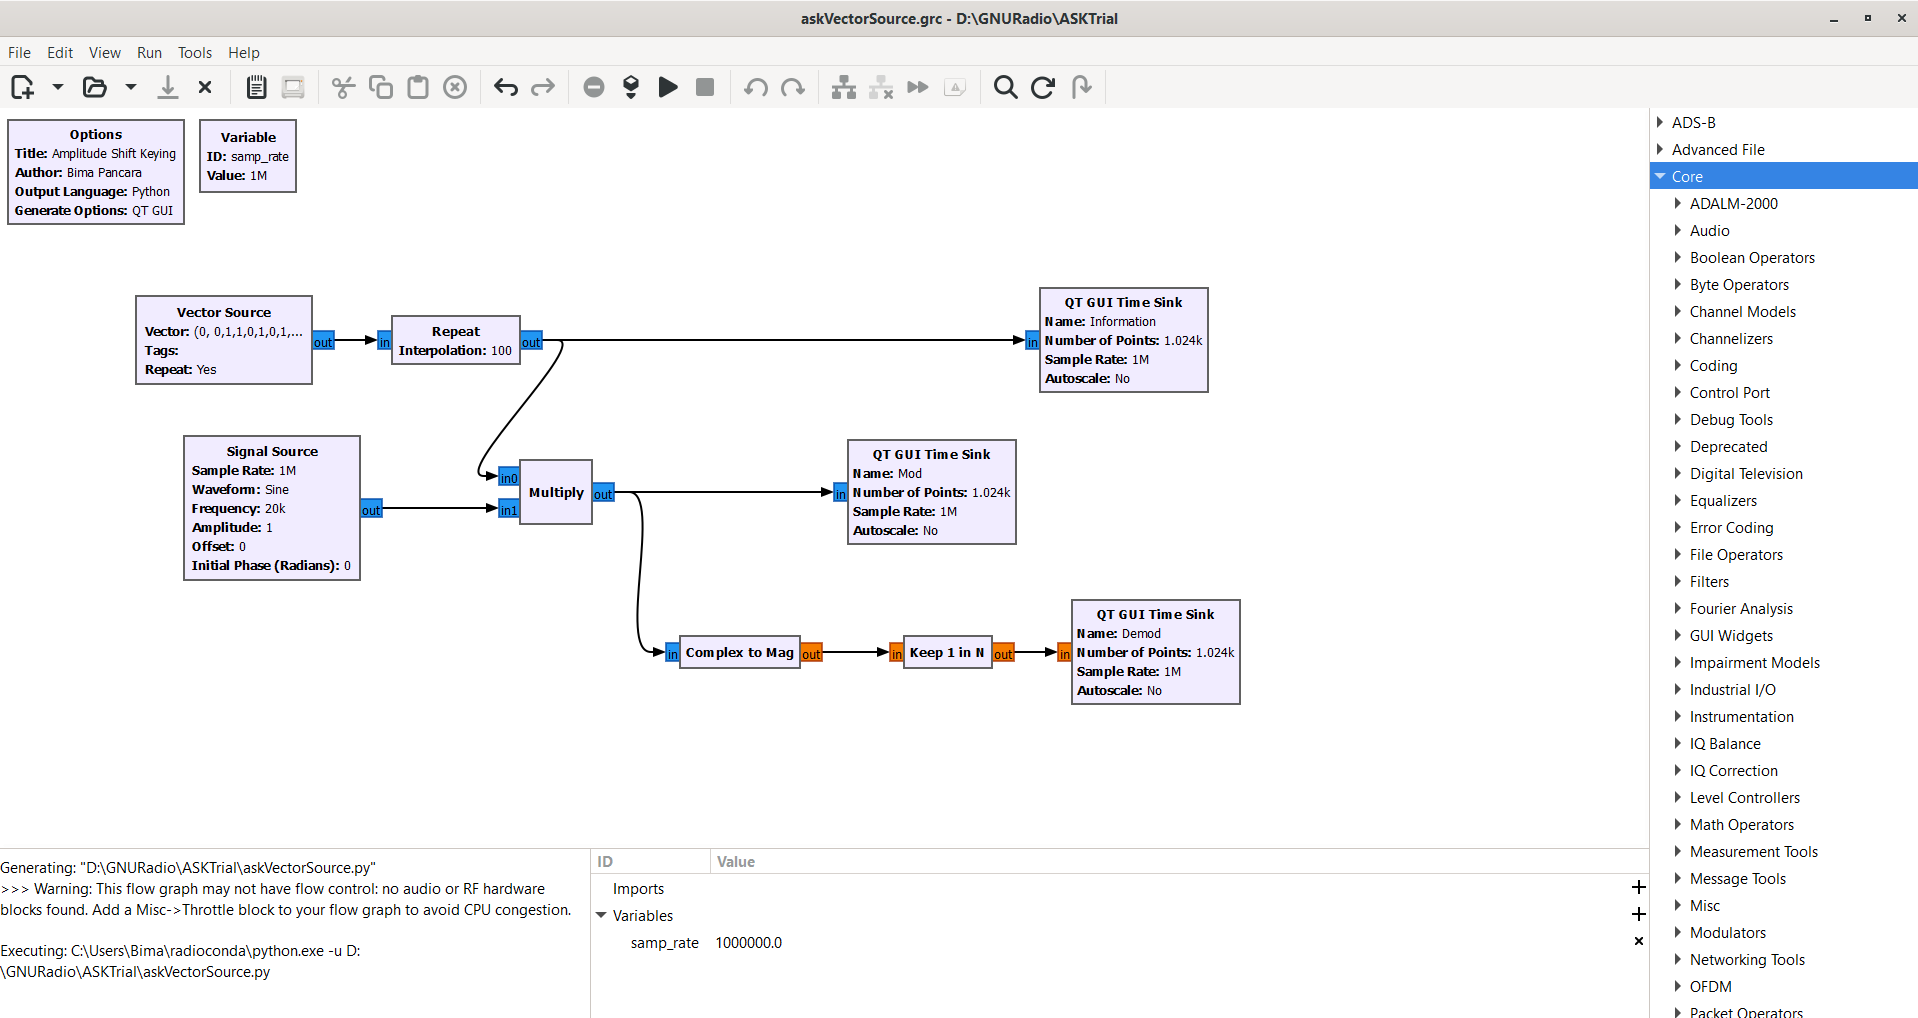
\includegraphics[scale=0.35]{pics/bab2/blokDiagramGRC.png} 
		\caption[Contoh \textit{Flowgraph} GNURadio]{Contoh \textit{Flowgraph} GNURadio}
		\label{pic:contohBlokGRC}
	\end{center}
\end{figure}

Gambar \ref{pic:contohBlokGRC} adalah contoh blok diagram sistem (\textit{flowgraph}) yang sukses dibuat pada aplikasi GNURadio. Pada gambar \ref{pic:contohRunGRC} menunjukkan hasil bila desain sistem tersebut dijalankan.

\begin{figure}
	\begin{center}
		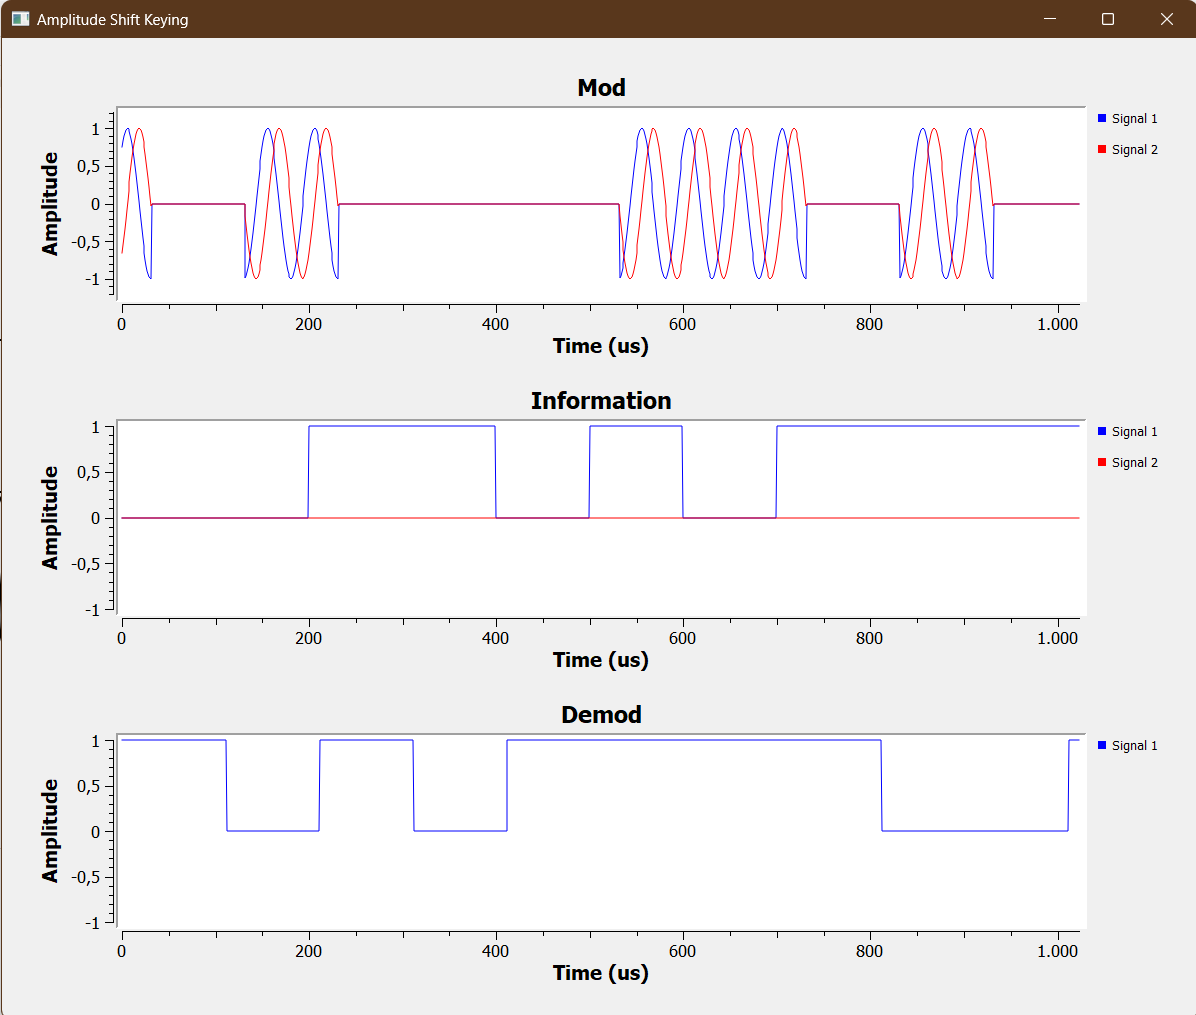
\includegraphics[scale=0.4]{pics/bab2/contohRunGRC.png} 
		\caption[Contoh Hasil Desain Sistem GNURadio]{Contoh Hasil Desain Sistem GNURadio}
		\label{pic:contohRunGRC}
	\end{center}
\end{figure}




% Bab 3 : Metodologi Penelitian
%-----------------------------------------------------------------------------%
\chapter{\babTiga}
%-----------------------------------------------------------------------------%

%-----------------------------------------------------------------------------%
\section{Alur Penelitian}
%-----------------------------------------------------------------------------%
Dalam suatu penelitian, terdapat urutan tahapan yang perlu dilakukan. Alur penelitian ini mengandung seluruh langkah yang harus ditempuh, mulai dari fase perancangan hingga tahap akhir penelitian.
 \begin{figure}
	\begin{center}
		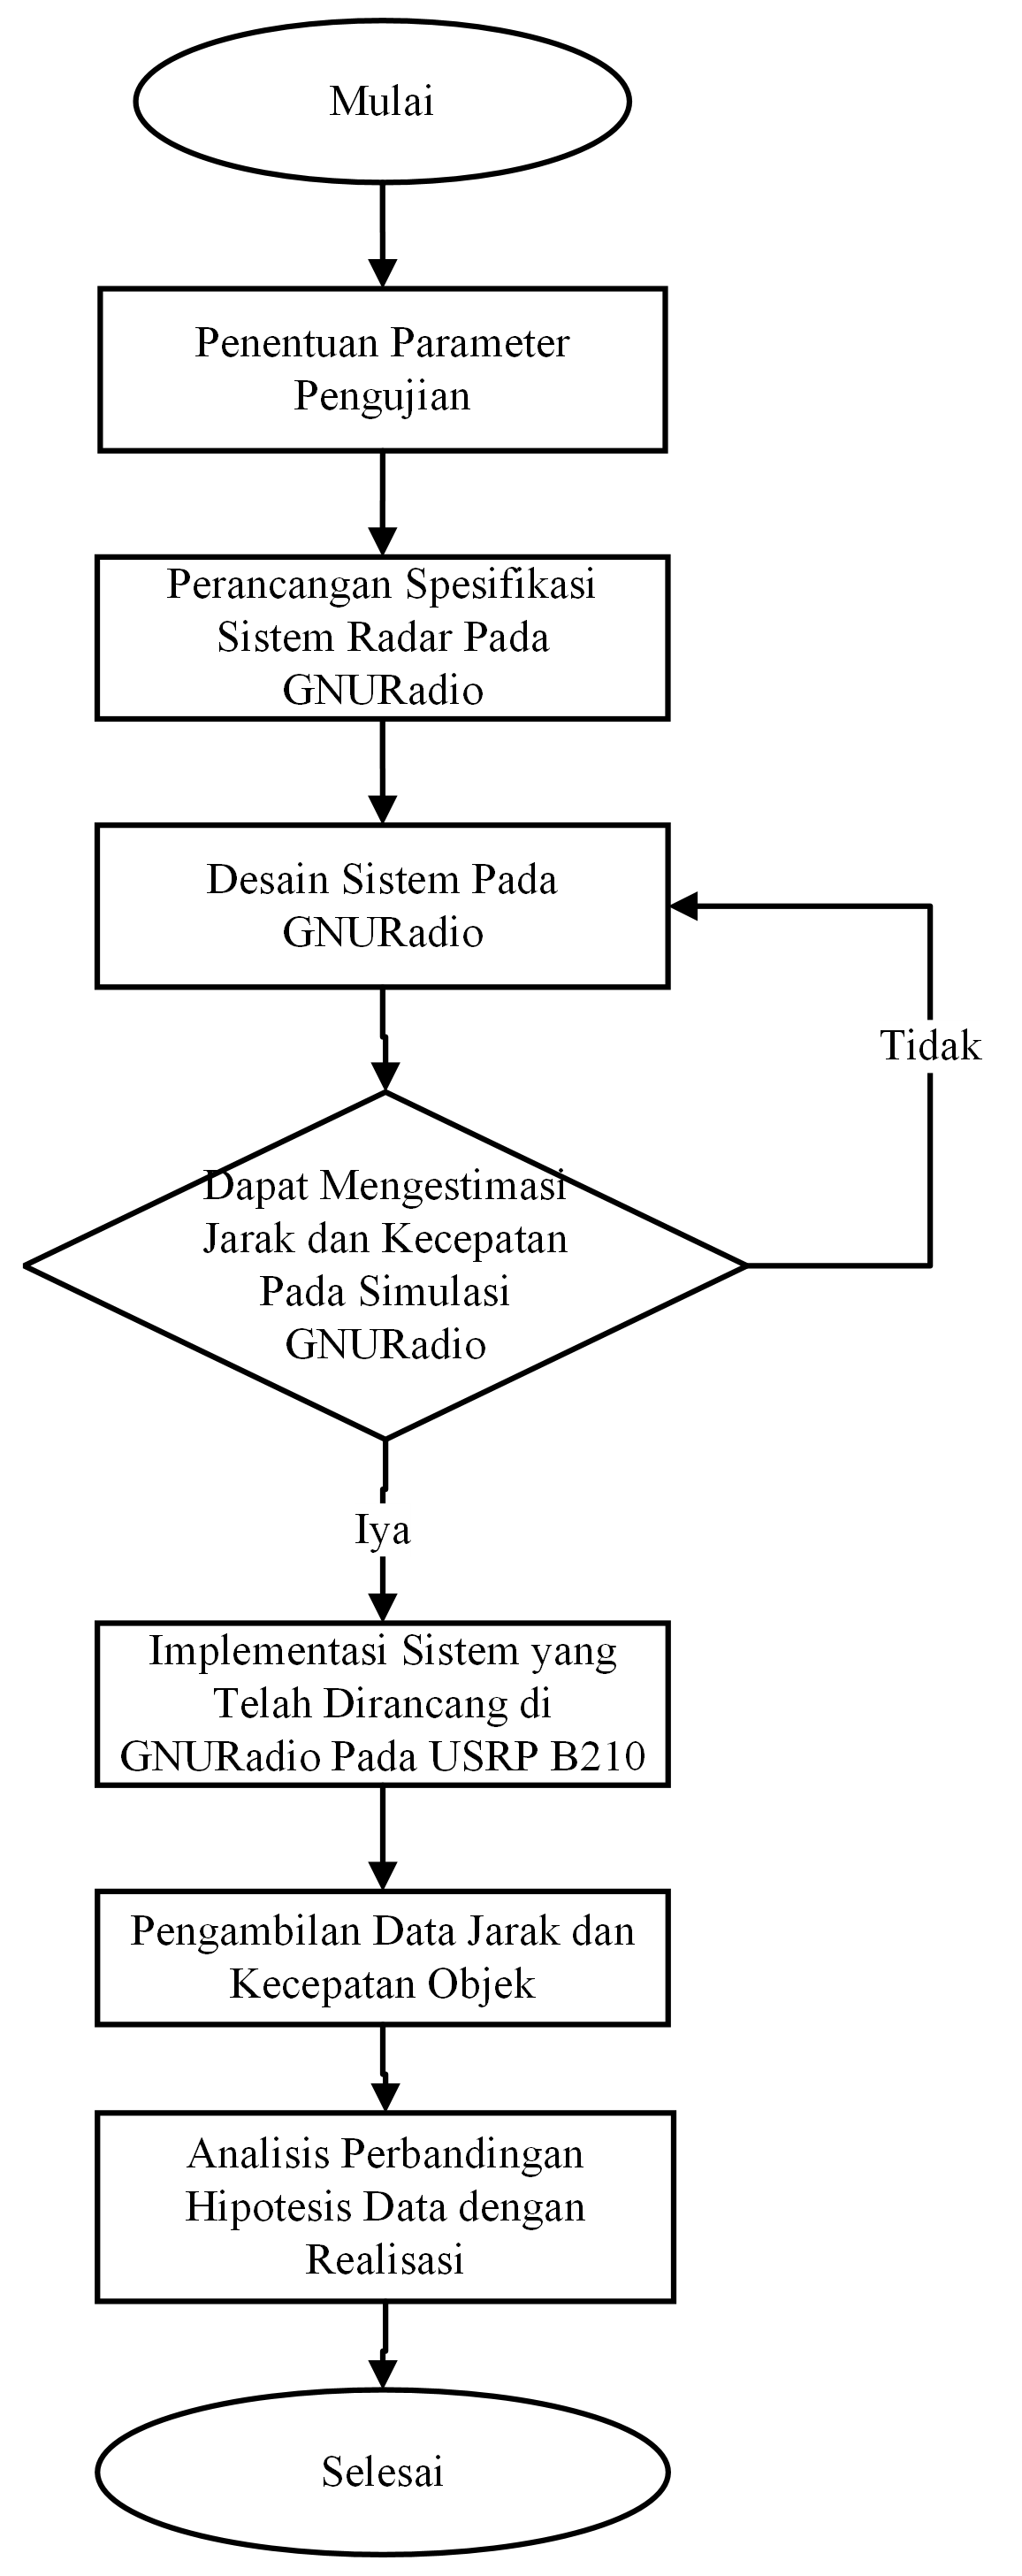
\includegraphics[scale=0.53]{pics/bab3/FlowchartTugasAkhir.png} 
		\label{img:flowchart}
		\caption[\textit{Flowchart} Penelitian]{\textit{Flowchart} Penelitian}
	\end{center}
\end{figure}
Pada alur penelitian yang telah dirancang, terdapat beberapa tahap yang perlu dilakukan setelah penelitian dimulai dan sebelum penelitian diakhiri. Tiap tahapan yang telah dirancang harus dilaksanakan sebaik mungkin agar hasil yang diharapkan dapat tercapai.
	
\section{Penentuan Parameter}

Pada tahap ini parameter pengujian ditentukan sehingga hasil yang dicapai dapat dikatakan baik, sebagai berikut.

\begin{center}
	\begin{longtable}{| c | c | c |}
		\caption{Parameter Pengujian}
		\label{tab:paramUji}\\
		\hline
		No. & Parameter Pengujian		& Satuan\\ \hline
		1.  &Jarak	   					& m\\
		2.  &Kecepatan 					& m/s\\
		3.  &\textit{RMSE}				& -\\
		4.	&Nilai prediksi \textit{beat frequency}	& Hz \\
		5.	&Nilai prediksi \textit{doppler frequency shift} & Hz \\
		\hline
	\end{longtable}
\end{center}

\section{Perancangan Spesifikasi Sistem}
Pada tahap ini, dilakukan perancangan sistem radar. Maka perlu ditentukannya spesifikasi radar berdasarkan perangkat keras USRP berseri B210 yang digunakan.  Spesifikasi dari sistem ini akan dijelaskan pada tabel berikut.

\begin{center}
	\begin{longtable}{| c | c | c |}
		\caption{Spesifikasi Sistem Radar}
		\label{tab:spekRadar}\\
		\hline
		No. & Spesifikasi 								& Keterangan\\\hline
		1.  & USRP 										& B210\\
		2.  & \textit{Carrier Frequency} ($F_{c}$) 		& 3100 MHz \\
		3.  & \textit{Bandwidth} 	(BW)				& 50 MHz \\
		4.	& Frekuensi \textit{Sampling}	($F_{s}$)	& 30 MHz	\\
		5.	& Bentuk Modulasi							& \textit{Triangular}\\
		6.  & Jarak Maksimum 		($R_{max}$)			& 145.16 km \\
		7.  & Resolusi Jarak 		($R_{res}$)			& 3 m \\
		8.  & Kecepatan Maksimum	($V_{max}$)			& 15 $m/s$ \\
		9.  & Resolusi Kecepatan 	($V_{res}$)			& 1 $m/s$\\
		10.	& Durasi \textit{Chirp}	($T_{c}$)			& 1613 $\mu s$\\
		11.	& \textit{Chirp Rate}	($\mu$)				& 0.031 $MHz/\mu s$\\
		12. & Durasi \textit{frame}	($T_{f}$)			& 48 ms \\
		\hline
	\end{longtable}
\end{center}

\begin{itemize}
	\item Hitung panjang gelombang ($\lambda$) dari frekuensi pembawa yang sudah ditentukan yaitu 3.1 GHz.
	\begin{align*}
		\lambda &= \frac{c}{F_{c}}\\
		\lambda &= \frac{3 \cdot 10^{8}}{3.1 \cdot 10^{9}}\\
		\lambda &= 0.0967 m
	\end{align*}

	\item Menghitung resolusi jarak berdasarkan persamaan \ref{eq:RangeRes} dan dengan menentukan \textit{bandwidth} bernilai 50 MHz, maka.
		\begin{align*}
			R_{res} &= \frac{c}{2 BW} \\
			R_{res} &= \frac{3 \cdot 10^{8}}{2 \cdot 50}\\
			R_{res} &= 3 m
		\end{align*}
	\item Menghitung jarak maksimum yang dapat dideteksi oleh radar digunakanlah persamaan \ref{eq:MaxRange}, namun sebelumnya harus ditentukan terlebih dahulu nilai $\mu$, yang merupakan tingkat kenaikan frekuensi pada suatu periode sesuai dengan persamaan \ref{eq:chirpRate}, dengan nilai $T_{c}$ sesuai persamaan \ref{eq:chirpTime} dan nilai kecepatan maksimum ditentukan bernilai 15 m/s, maka.
	
	\begin{align*}
		T_{c} &= \frac{\lambda}{4 \cdot V_{max}}\\
		T_{c} &= \frac{0.0967}{4 \cdot 15}\\
		T_{c} &= 1613 \mu s
	\end{align*}

	\item 
	Sehingga nilai \textit{chirp rate} ($\mu$) dapat dihitung menjadi.

		\begin{align*}
		\mu &= \frac{\textit{Bandwidth}}{T_{c}}\\
		\mu &= \frac{\textit{50}}{1613}\\
		\mu &= 0.031 MHz/ \mu s
		\end{align*}

	\item 	
	Dengan jarak maksimum yang didapat adalah.
		\begin{align*}
		R_{max} &= \frac{F_{s} \cdot c}{2 \cdot \mu}\\
		R_{max} &= \frac{30 \cdot 10^{6} \cdot 3 \cdot 10^{8}}{2 \cdot 0.031}\\
		R_{max} &= 145.16 km
		\end{align*}

	\item 
	Dengan $T_{f}$ sebagai durasi \textit{frame} bernilai 0.048 s maka resolusi kecepatannya.
		\begin{align*}
			V_{res} &= \frac{\lambda}{2 \cdot T_{f}}\\
			V_{res} &= \frac{0.0967}{2 \cdot 0.048}\\
			V_{res} &= 1 m/s
		\end{align*}

\end{itemize}

\section{Implementasi Sistem}
Tahap implementasi ini dilakukan pada aplikasi GNURadio dan menghasilkan \textit{flow diagram} yang merepresentasikan langkah yang dilakukan pada USRP. \textit{Flow diagram} yang didesain sudah memenuhi spesifikasi sistem radar pada tabel \ref{tab:spekRadar}. 

Implementasi sistem akan dilaksanakan pada beberapa perangkat, mulai dari laptop, antena, dan USRP. Berikut detail perangkat yang akan digunakan pada saat implementasi guna mendapat hasil yang baik.

\begin{enumerate}
	\item \textit{IdeaPad Gaming 3 15ARH7} :
	\begin{figure}
		\begin{center}
			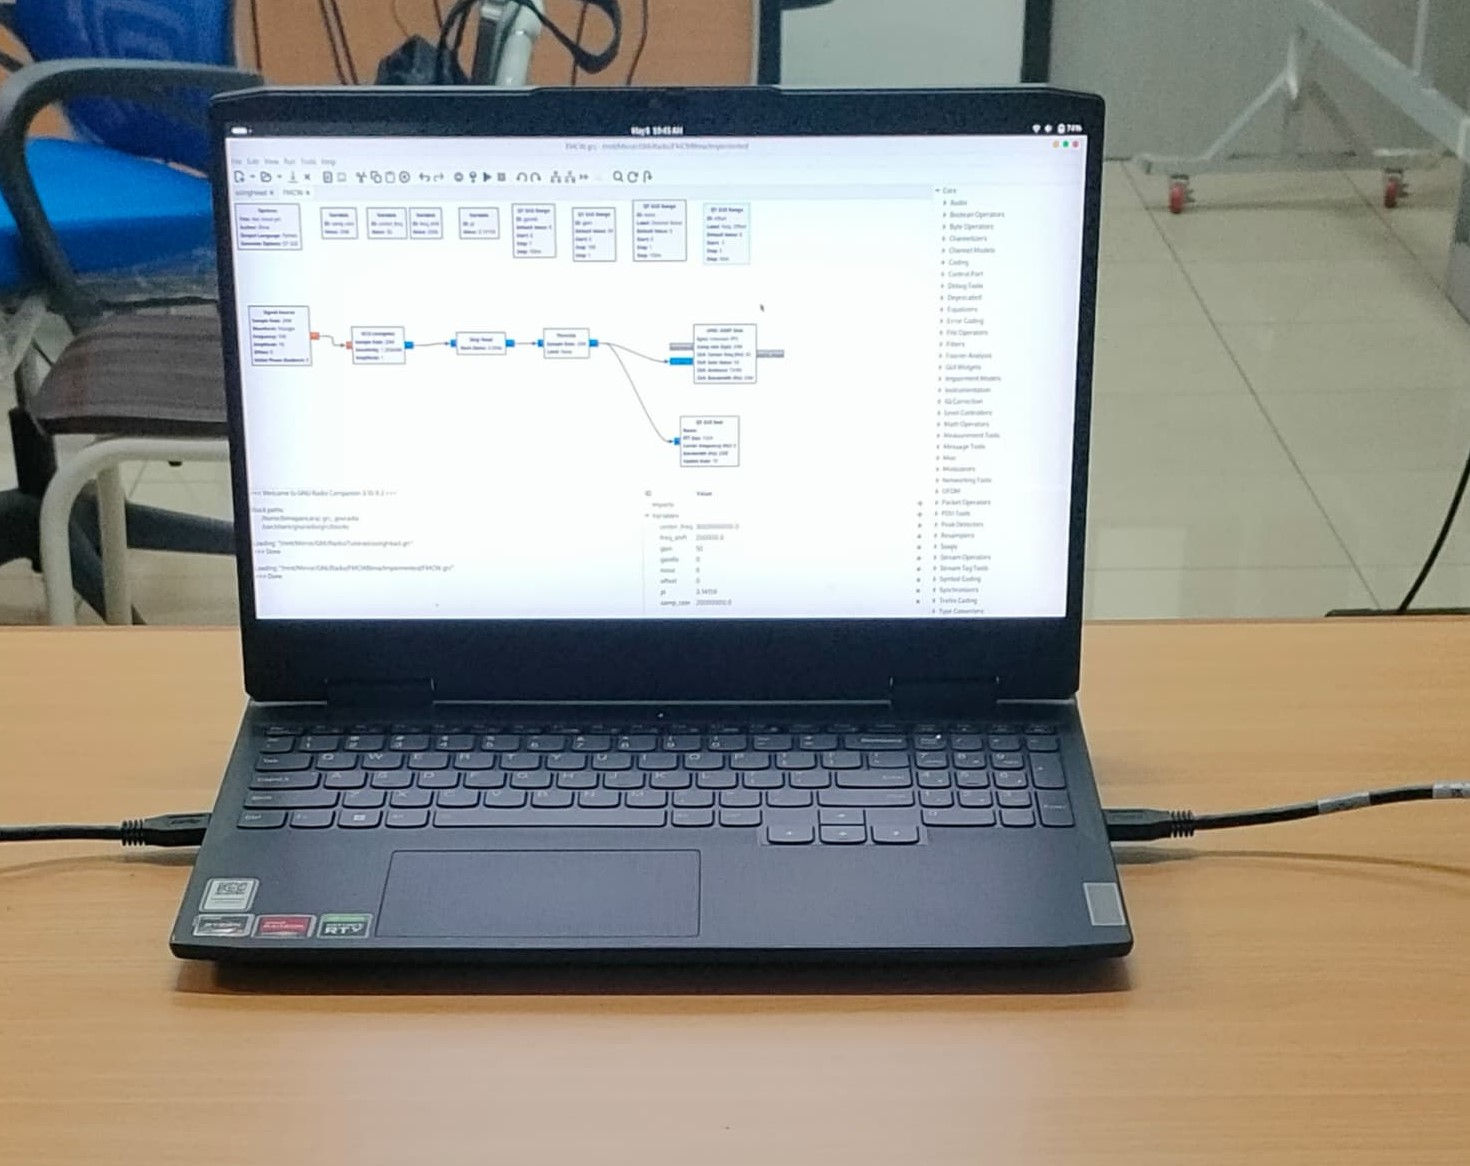
\includegraphics[scale=0.2]{pics/bab3/laptop.jpg} 
			\caption[Gambar Perangkat Laptop Yang Digunakan]{Gambar Perangkat Laptop Yang Digunakan}
			\label{pic:contohBlokGRC}
		\end{center}
	\end{figure}

	\begin{itemize}
		\item \textit{Processor} : AMD Ryzen 7 6800H dengan \textit{Radeon Graphics} 3.20 GHz
		\item \textit{Memory} : 8,00 GB (7,19 GB \textit{usable})
	\end{itemize}

	\item Perangkat \textit{Software Defined Radio} :
	\begin{figure}
		\begin{center}
			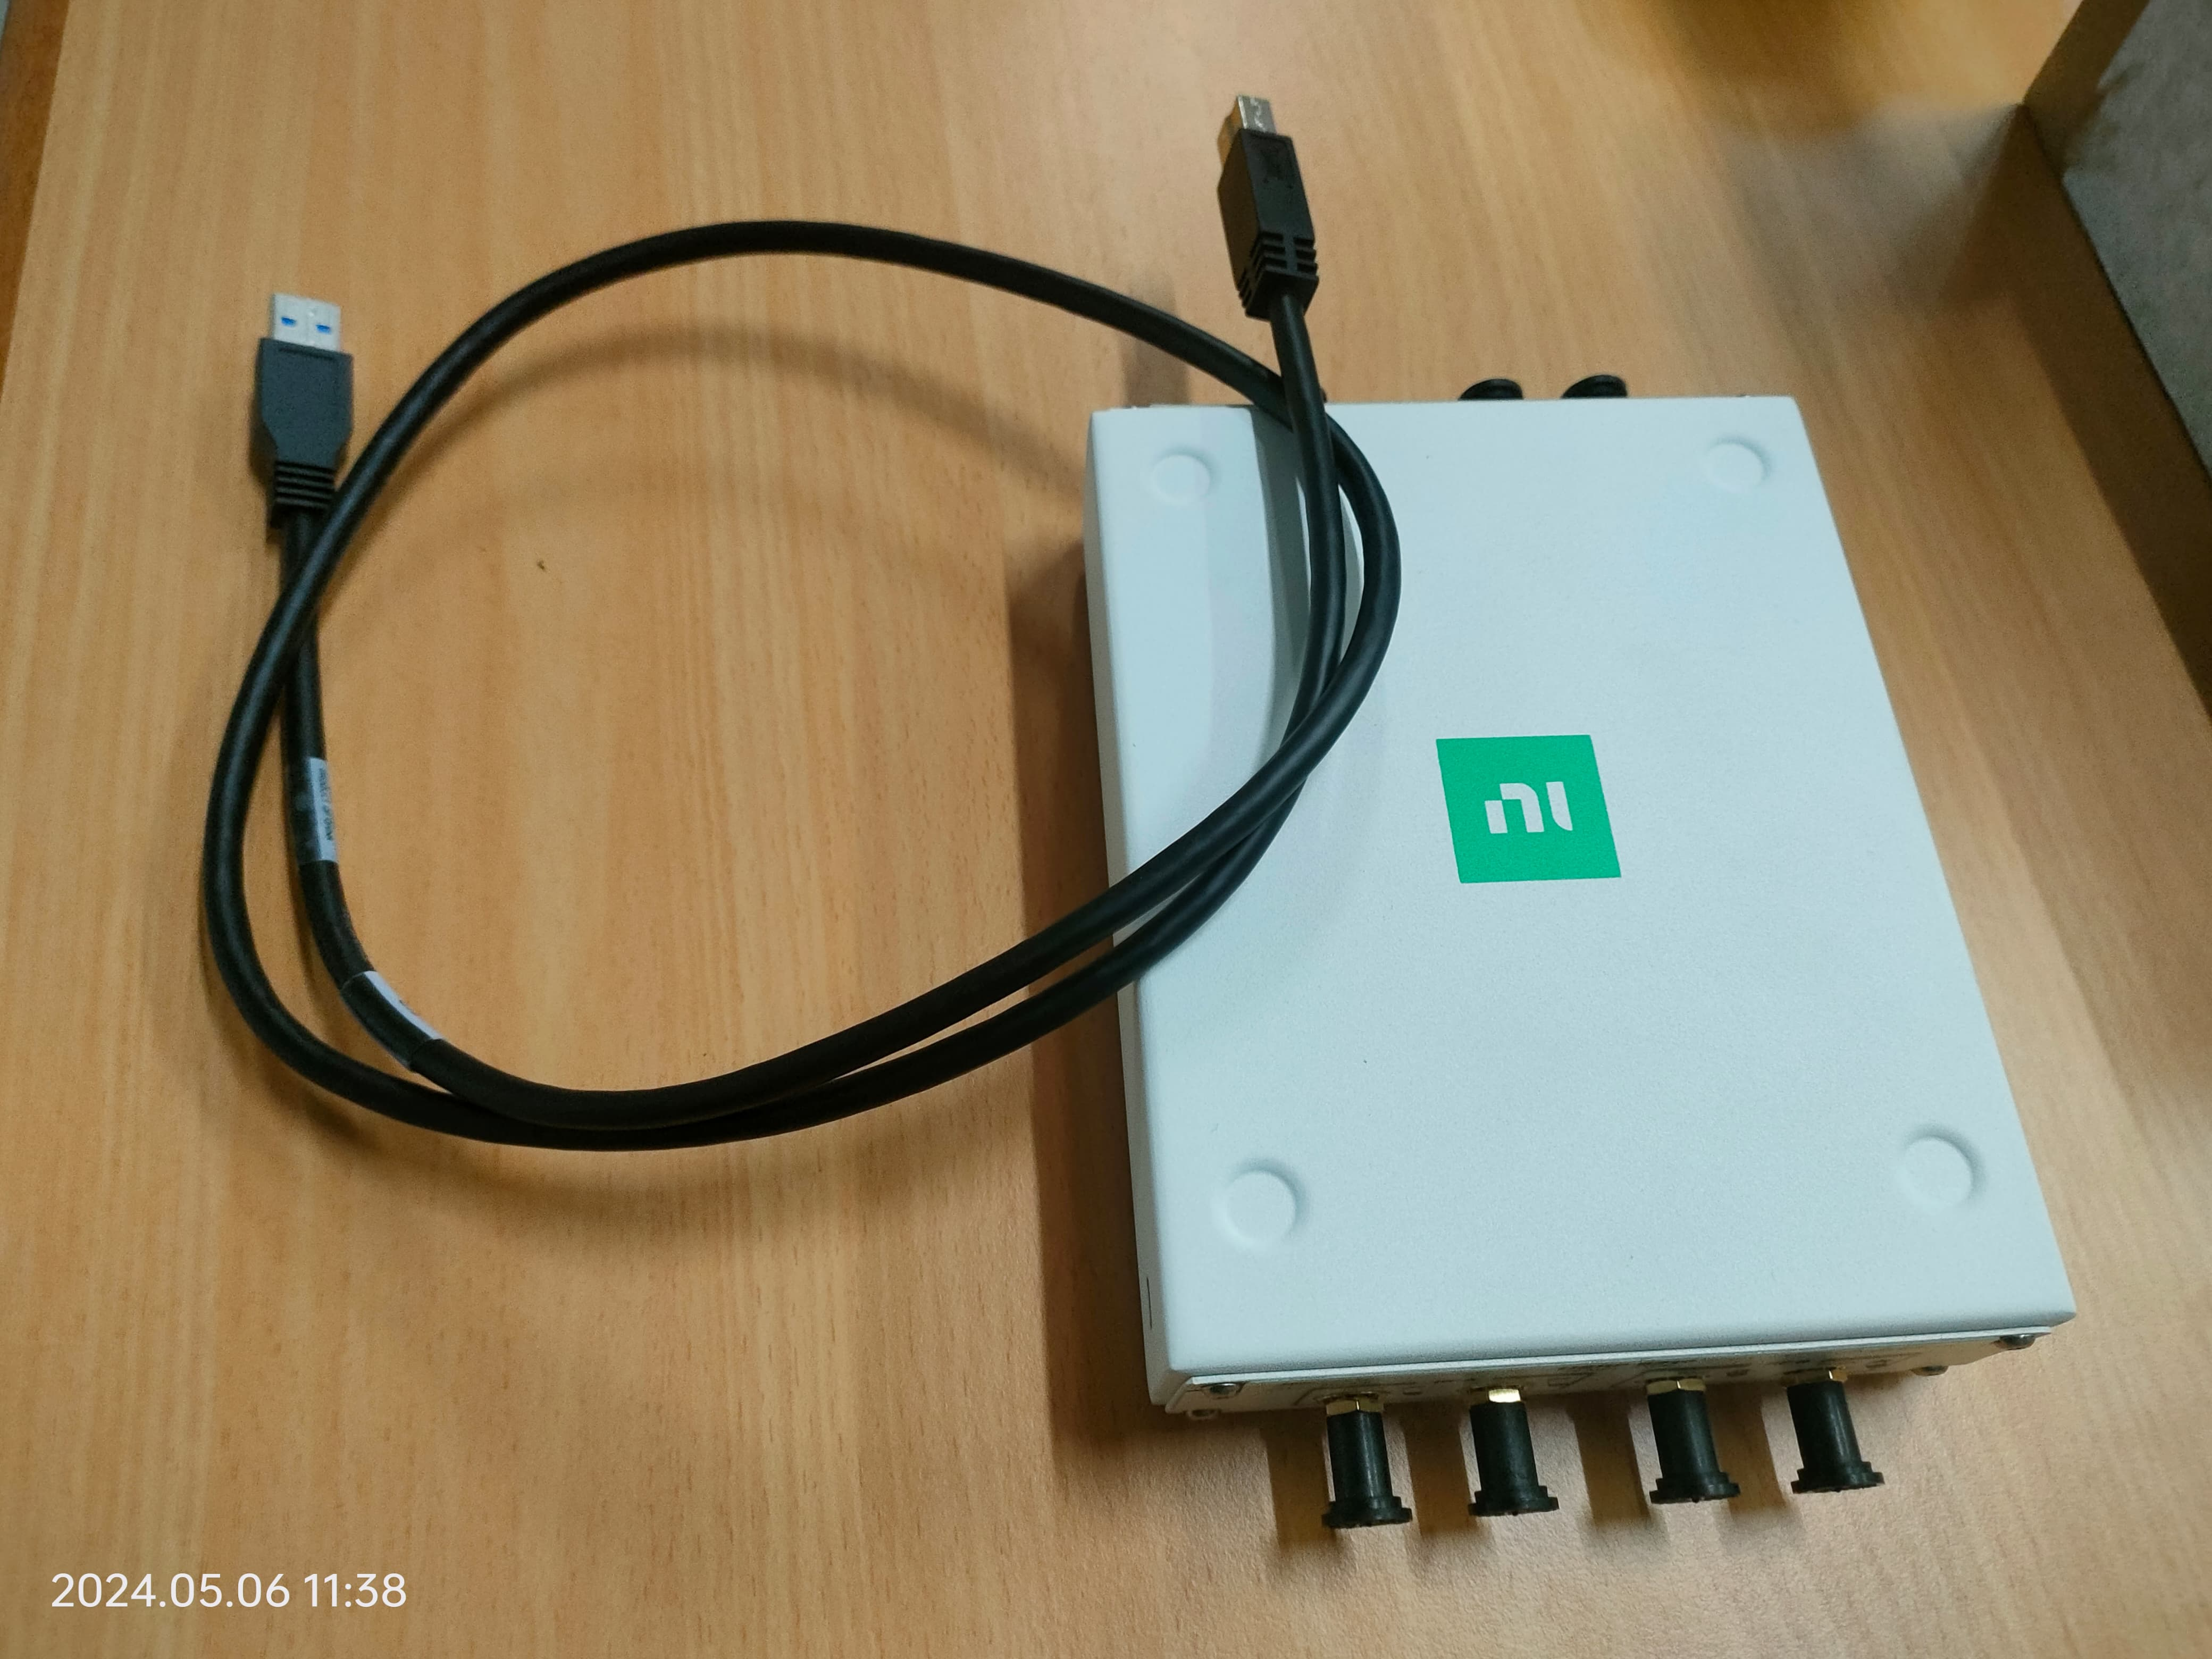
\includegraphics[scale=0.045]{pics/bab3/usrp2.jpg}
			\caption{Alat USRP B210}
			\label{img:logPeriodic}
		\end{center}
	\end{figure}
	\begin{itemize}
		\item Tipe : USRP B210 
		\item Jarak Frekuensi : 70 MHz - 6000 MHz 
	\end{itemize}

	\item Antena \textit{Log-periodic} :
	\begin{figure}
		\begin{center}
			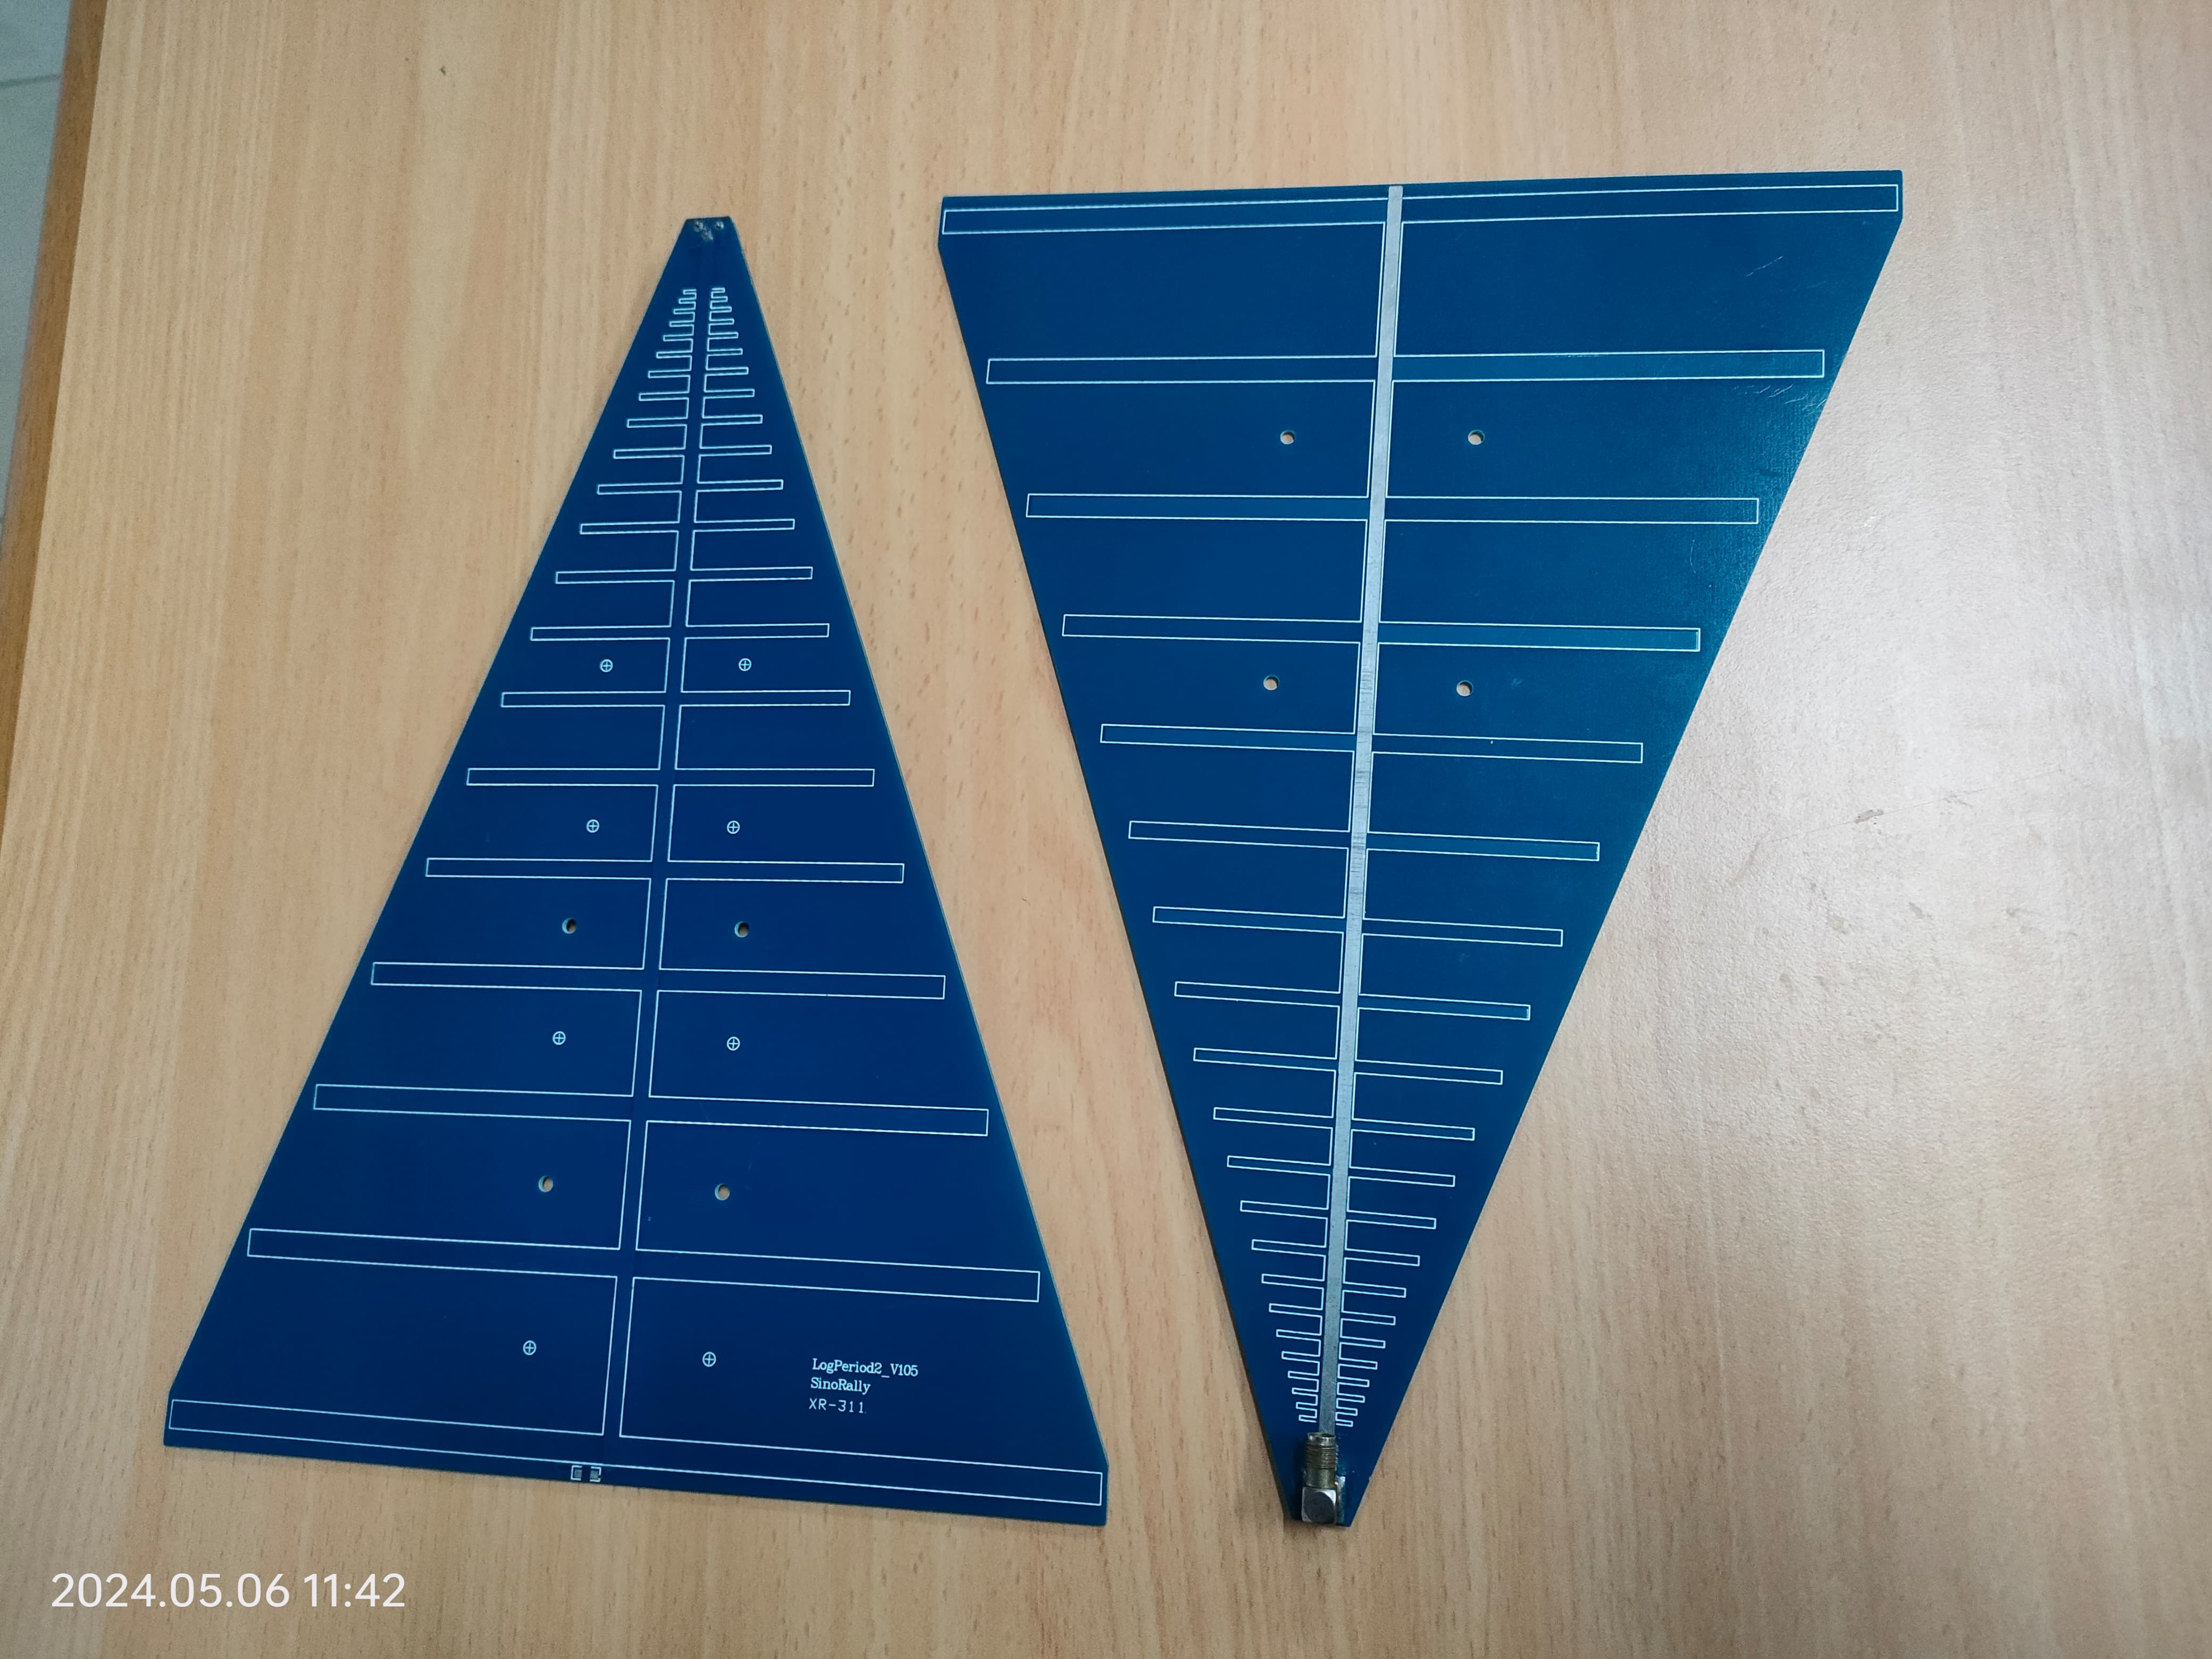
\includegraphics[scale=0.05]{pics/bab3/logPeriodic.jpg}
			\caption{Antena \textit{Log Periodic} Pengujian}
			\label{img:usrpBoard}
		\end{center}
	\end{figure}
	\begin{itemize}
		\item Frekuensi : 800 MHz - 6000 MHz 
		\item Pola Radiasi : \textit{Directional}
		\item \textit{Gain} : 5.2 - 6.3 dB
	\end{itemize}
\end{enumerate}

	
\section{Pengambilan Data}
Pada tahap ini, pengambilan data dengan radar yang sudah didesain dan diimplementasikan pada USRP dilakukan. Pengujian dilakukan dengan menggunakan kendaraan roda empat sebagai objek yang akan dideteksi. Sehingga pengambilan data kecepatan dan prediksi jarak dapat dilakukan. Hasil prediksi jarak dan kecepatan radar akan dibandingkan dengan nilai aktual jarak pada kenyataan dan kecepatan tercatat pada \textit{speedometer}.

\begin{figure}
	\begin{center}
		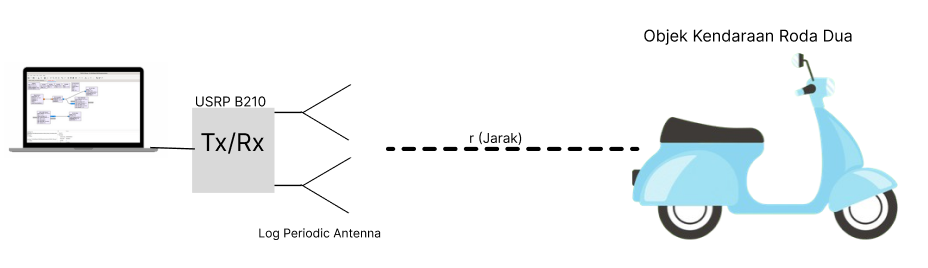
\includegraphics[scale=0.55]{pics/bab3/skema.png}
		\caption{Skema Penelitian}
		\label{img:skema}
	\end{center}
\end{figure}

Data berupa nilai \textit{beat frequency} dan \textit{doppler frequency shift} yang sudah ditentukan sebagai parameter pengujian telah didapat dari hasil pengambilan data akan dibandingkan dengan nilai prediksi berdasarkan perhitungan. Dengan begitu, maka nilai RMSE dapat dihitung.

\begin{figure}
	\begin{center}
		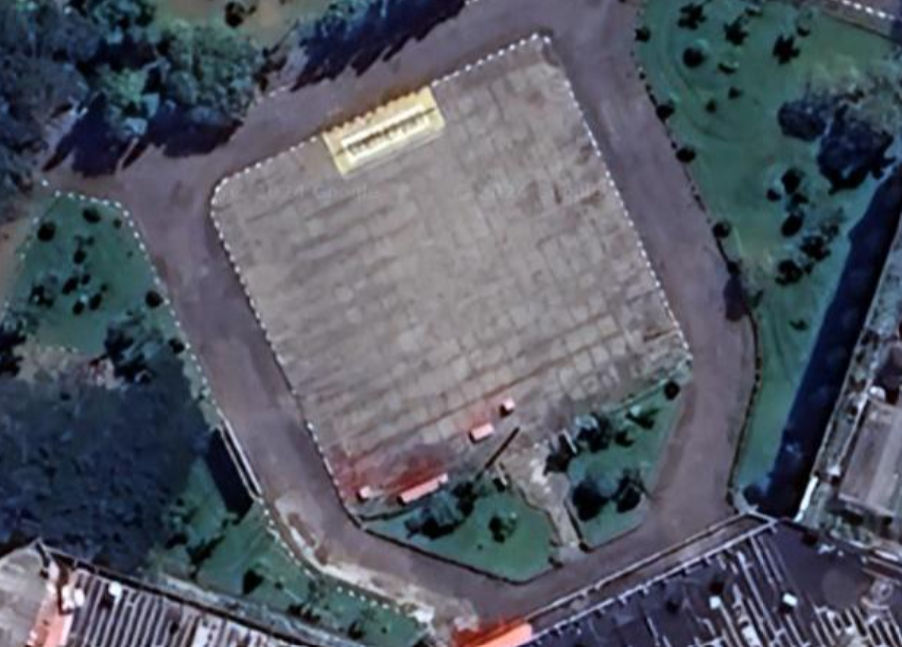
\includegraphics[scale=0.35]{pics/bab3/petaPengujian.png}
		\caption{Lokasi Pengujian}
		\label{img:petaUji}
	\end{center}
\end{figure}

Pengambilan data akan dilaksanakan di lokasi lapangan Universitas Telkom Surabaya yang beralamat Jl. Ketintang No.156, Ketintang, Kec. Gayungan, Surabaya, Jawa Timur 60231.

\section{Konfigurasi Pengujian}
Konfigurasi pengujian dilakukan sesuai dengan gambar \ref{img:skema}. Terdapat satu buah perangkat laptop yang terhubung dengan dua buah USRP, masing-masing USRP terhubung dengan antena \textit{Log-periodic}. USRP 1 berperan sebagai \textit{transmitter} sedangkan USRP 2 berperan sebagai \textit{receiver}.

\begin{figure}
	\begin{center}
		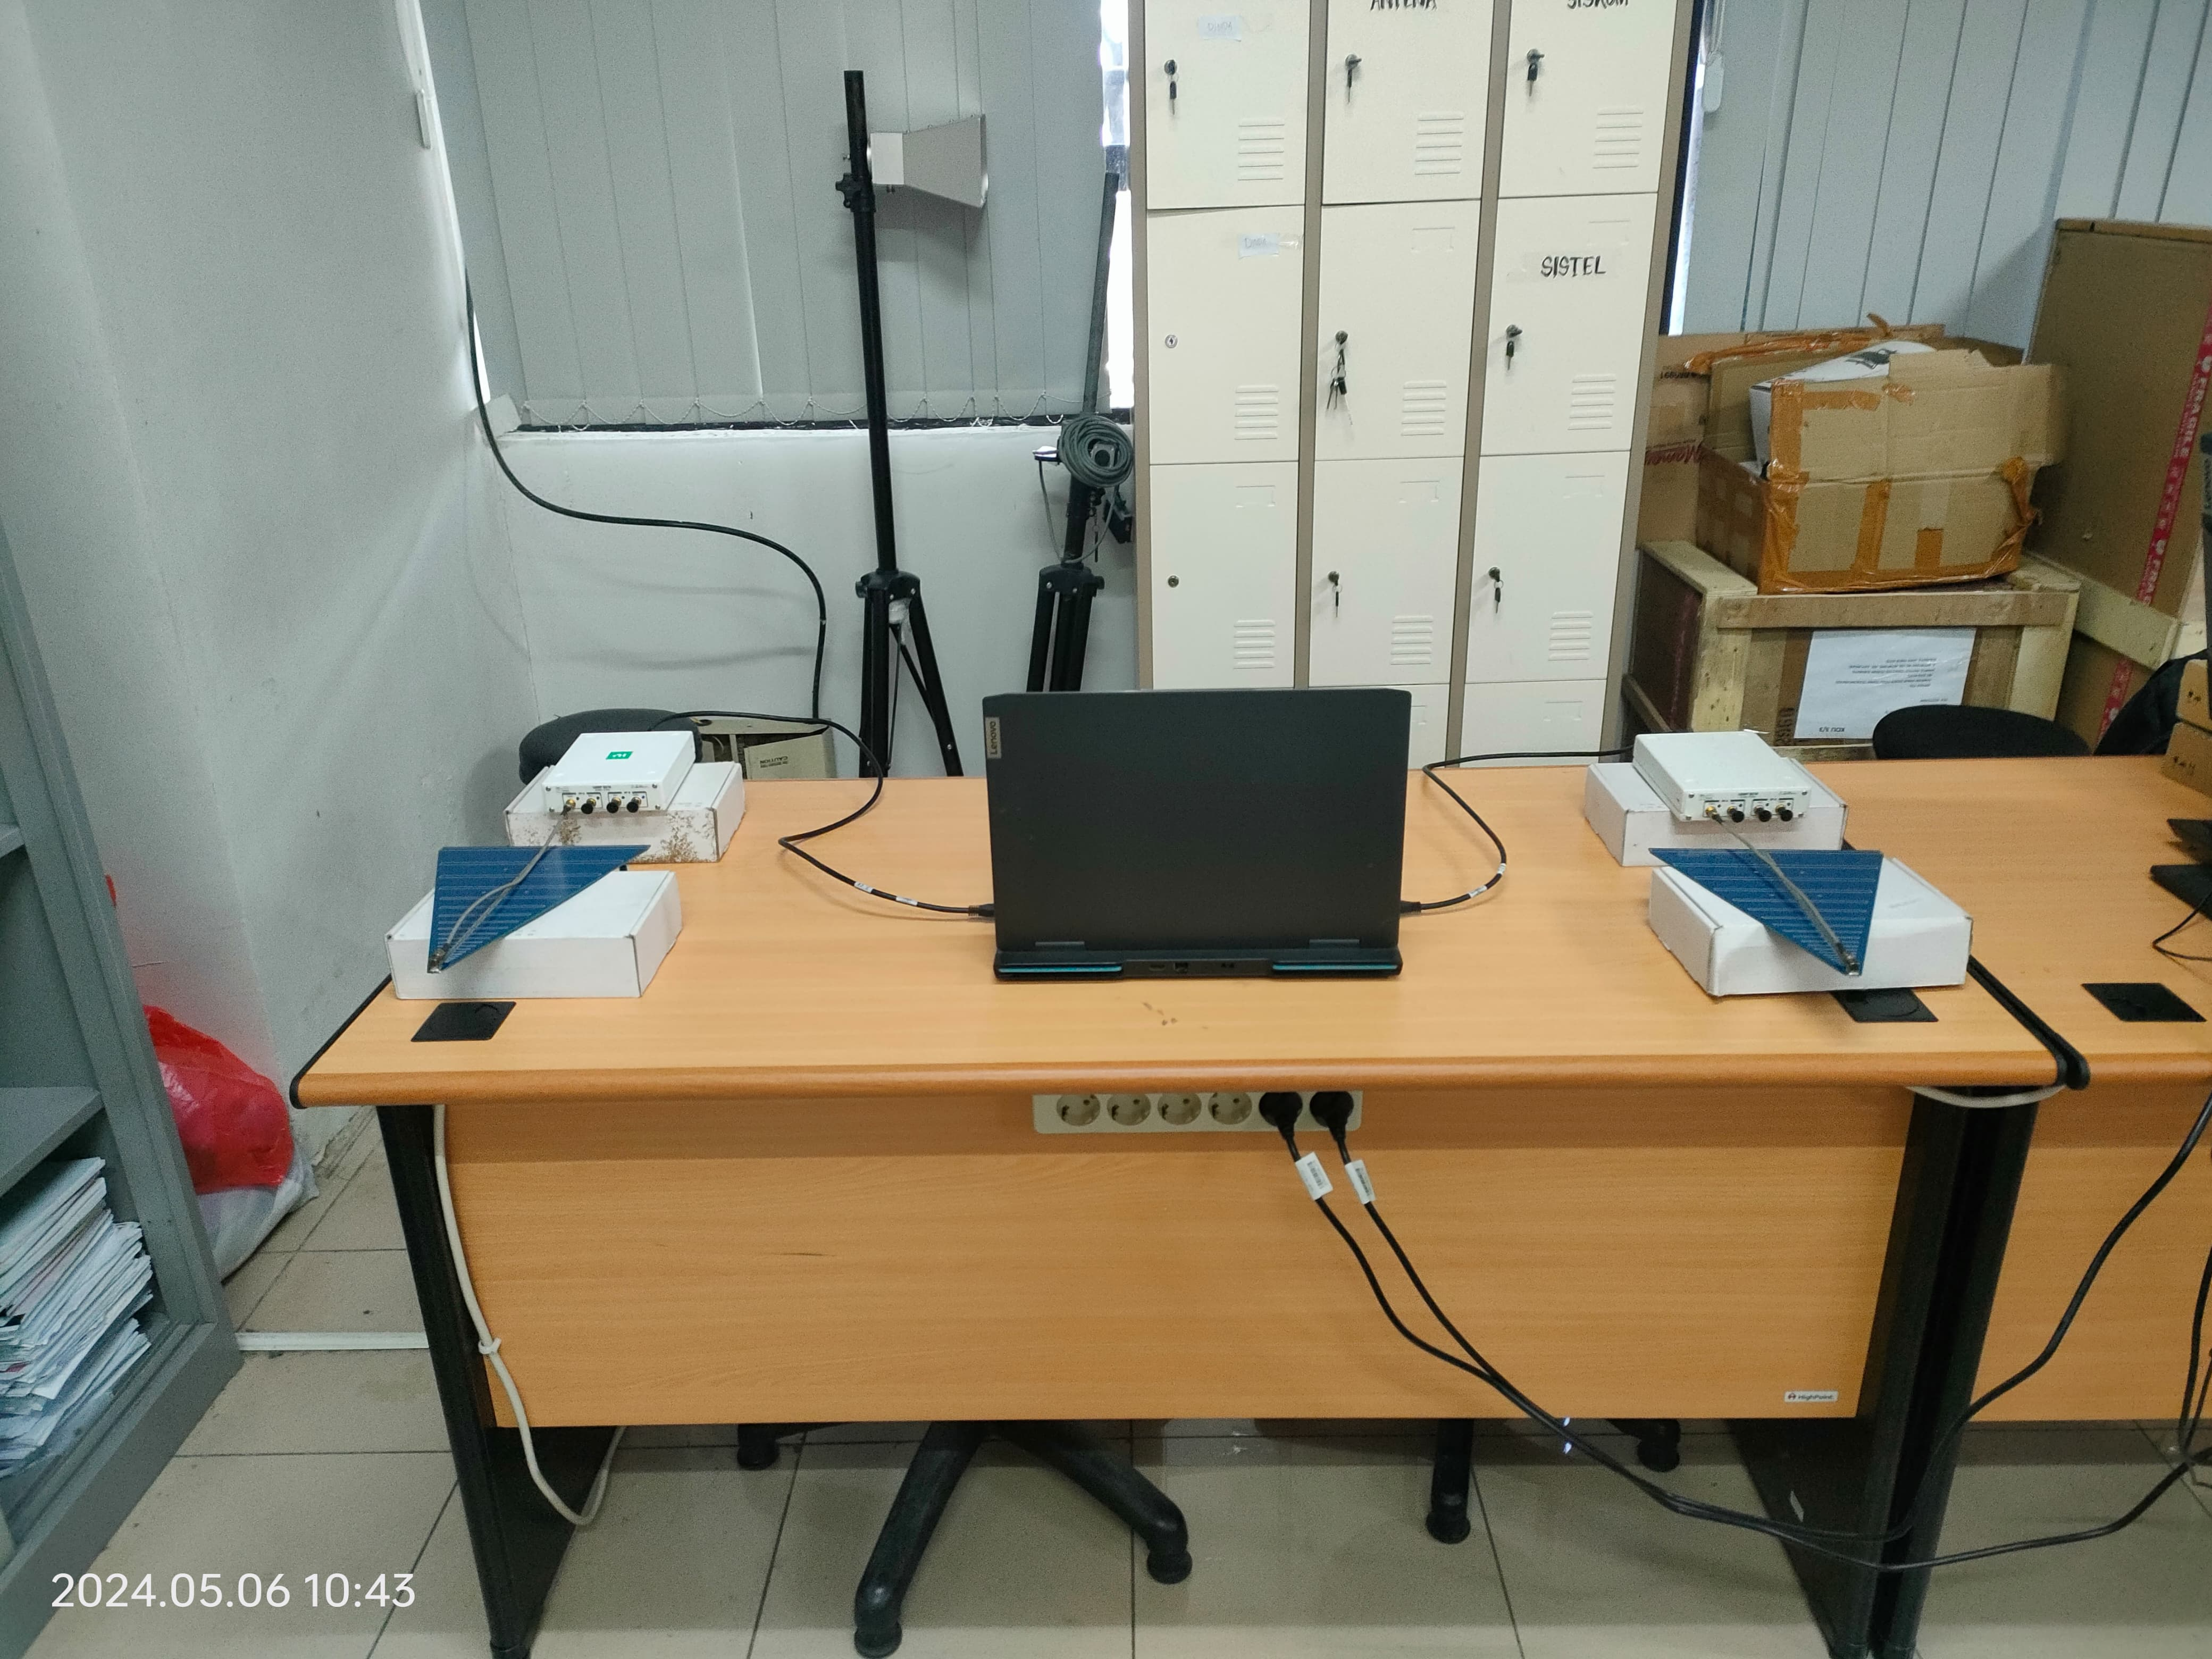
\includegraphics[scale=0.09]{pics/bab3/konfigurasiPengujian.jpg}
		\caption{Konfigurasi Pengujian}
		\label{img:konfigurasi}
	\end{center}
\end{figure}


\section{Prediksi Hasil Pengujian}

Prediksi hasil pengujian diperlukan untuk menjadi pembanding dari hasil yang akan didapat setelah melakukan pengujian. Perhitungan prediksi ini berupa nilai \textit{beat frequency} dan \textit{doppler frequency}. Prediksi nilai \textit{beat frequency} didapat pada persamaan \ref{eq:RangeEst} dan memodifikasinya dengan menentukan nilai jarak ($d_{0}$) pada estimasi jarak. Sehingga akan didapat persamaan estimasi \textit{beat frequency}($f_{b}$) seperti berikut.

\begin{equation}
	\nonumber
	f_{b} = \frac{d_{0} \cdot 2 \mu}{c} = \frac{d_{0} \cdot 2BW}{c \cdot T_{c}}
	\label{eq:predFb}
\end{equation}

Persamaan diatas menunjukkan bahwa dengan menentukan jarak ($d_{0}$) dalam meter, \textit{chirp rate} ($\mu$) dalam $Hz/\mu s$, kecepatan cahaya (c) dalam $m/s$, lebar pita frekuensi (BW) dalam Hz, dan waktu \textit{chirp} ($T_{c}$) dalam $\mu s$. Maka \textit{beat frequency} ($f_{b}$) yang ditemukan akan memiliki satuan Hz.


Prediksi nilai frekuensi doppler dapat dilakukan dengan mengubah persamaan \ref{eq:velocity} lalu memberikan asumsi nilai kecepatan (v) pada estimasi kecepatan dengan satuan m/s dan panjang gelombang frekuensi ($\lambda$) yang digunakan dengan satuan meter. Sehingga persamaan estimasi \textit{doppler frequency} ($f_{d}$) akan menjadi berikut.

\begin{equation}
	\nonumber
	f_{d} = \frac{v \cdot 2}{\lambda}
	\label{eq:predFd}
\end{equation}

Hasil prediksi dari nilai \textit{beat frequency} yang telah dihitung menggunakan turunan dari persamaan diatas berada pada tabel \ref{tab:predFbeat}.

\begin{center}
	\begin{longtable}{|c|c|}
		\caption{Prediksi Nilai \textit{Beat Frequency}}
		\label{tab:predFbeat}\\
		\hline
		d0 & Prediksi $f_{b}$  \\
		\hline
		5 m & 1033 Hz\\
		\hline
		10 m & 2067 Hz\\
		\hline
		15 m & 3100 Hz\\
		\hline
		20 m & 4133 Hz\\
		\hline
		25 m & 5167 Hz\\
		\hline
	\end{longtable}
\end{center}

Hasil prediksi dari nilai \textit{doppler frequency} yang didapat dengan persamaan \ref{eq:predFd} terdata dalam tabel \ref{tab:predFdopp}.

\begin{center}
	\begin{longtable}{|c|c|}
		\caption{Prediksi Nilai \textit{Doppler Frequency}}
		\label{tab:predFdopp}\\
		\hline
		v & Prediksi $f_{d}$  \\
		\hline
		3 m & 62 Hz\\
		\hline
		6 m & 124 Hz\\
		\hline
		9 m & 186 Hz\\
		\hline
		12 m & 248 Hz\\
		\hline
		15 m & 310 Hz\\
		\hline
	\end{longtable}
\end{center}
% Bab 4 : Pengumpulan dan pengolahan data
%-----------------------------------------------------------------------------%
\chapter{\babEmpat}
%-----------------------------------------------------------------------------%

\section{Desain Sistem}

Bagian ini menjelaskan tentang desain sistem yang dilakukan sesuai dengan spesifikasi sistem yang telah diajukan. Desain ini dibuat di perangkat lunak GNURadio.

\begin{figure}
	\centering
	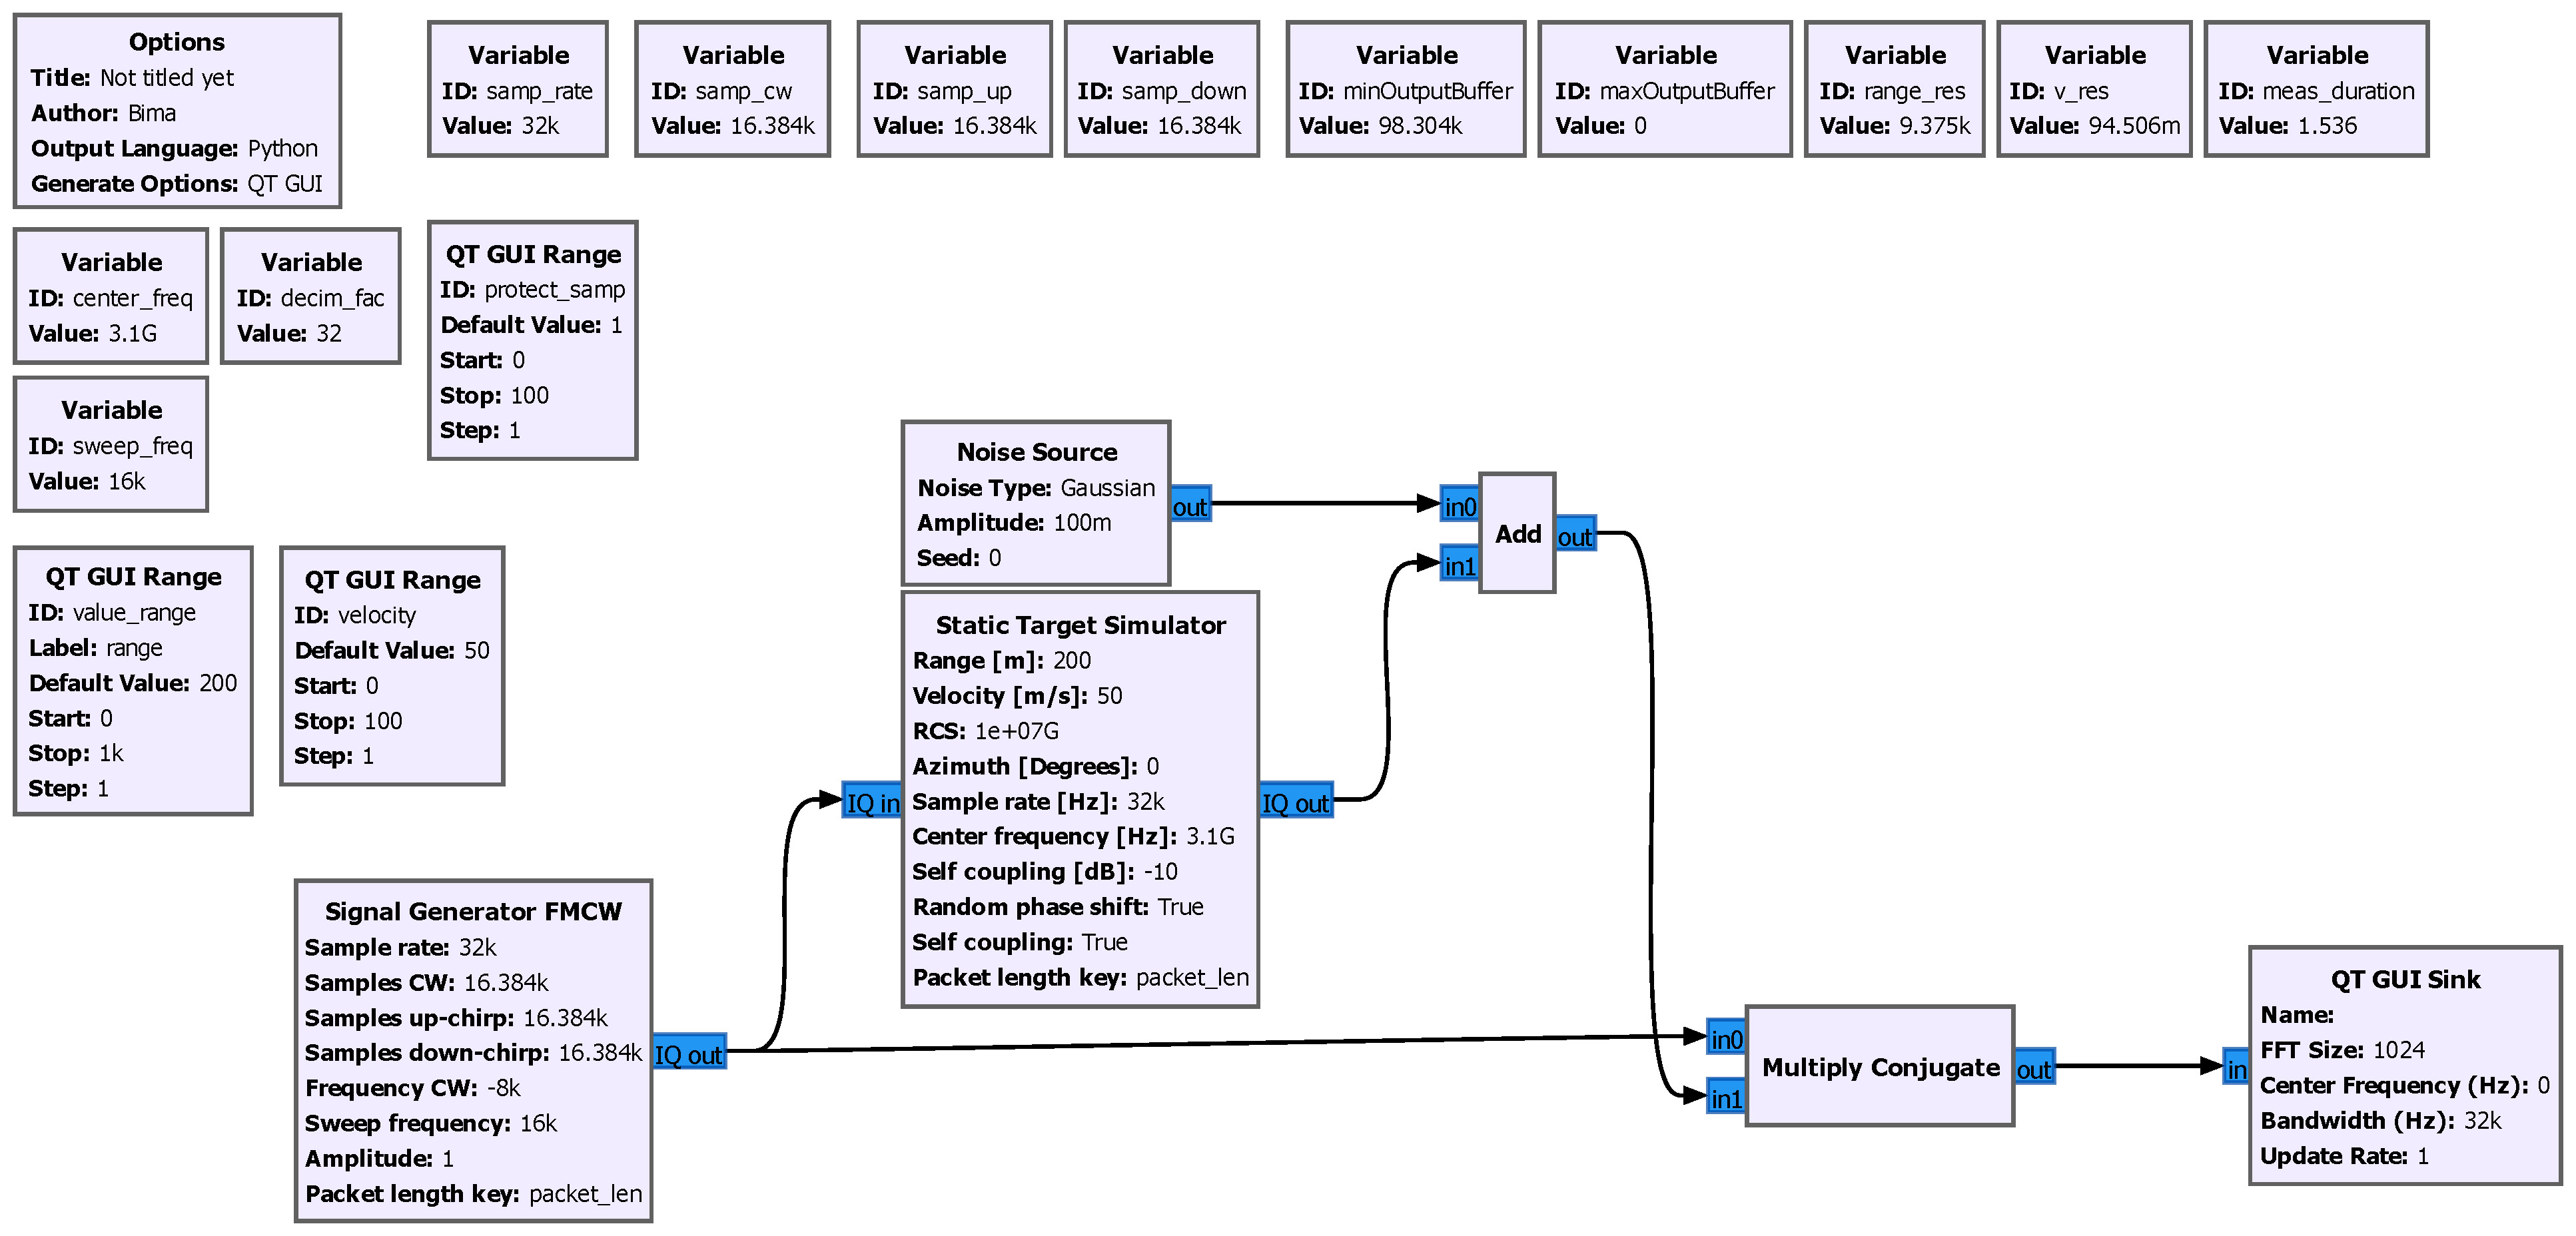
\includegraphics[scale=0.25]{pics/bab4/Simulasi.jpg}
	\caption{Desain Sistem Pada GNURadio}
	\label{fig:DesainSistem}
\end{figure}

Gambar~\ref{fig:DesainSistem} menunjukkan sistem pada GNURadio bila kalkulasi jarak dilakukan secara \textit{real-time}. Namun pada kenyataannya, saat pengukuran dilakukan, terjadi banyak sekali kegagalan, mulai dari \textit{error overflow} dan \textit{underflow}, \textit{error} pada pembacaan nilai jarak yang dihasilkan, hingga kalibrasi sinkronisasi perangkat yang perlu dilakukan tiap sistem diaktifkan.

Sehingga diputuskan bahwa pengambilan hasil dilakukan secara tidak \textit{real-time}, sehingga skema dari sistem yang digunakan di GNURadio berubah. Dalam pengambilan data tidak langsung, juga terjadi \textit{error overflow}, namun hal ini bisa dilewati dengan memanfaatkan kemampuan sistem operasi Linux untuk \textit{mount} dan menyimpan langsung di RAM.

%-----------------------------------------------------------------------------%
\section{Pengukuran Antena}
%-----------------------------------------------------------------------------%
Antena merupakan salah satu faktor penting dalam sistem radar, parameter seperti pola radiasi dan \textit{return loss} merupakan hal yang perlu dipertimbangkan dalam memilih antena. Pada penelitian ini, digunakan antena \textit{log periodic} dengan \textit{bandwidth} yang lebar. Antena identik digunakan sebagai \textit{transmitter} dan \textit{receiver}. Pola radiasi yang didapat pada pengujian antena adalah seperti gambar~\ref{fig:polaRadiasi}.

\begin{figure}
	\centering
	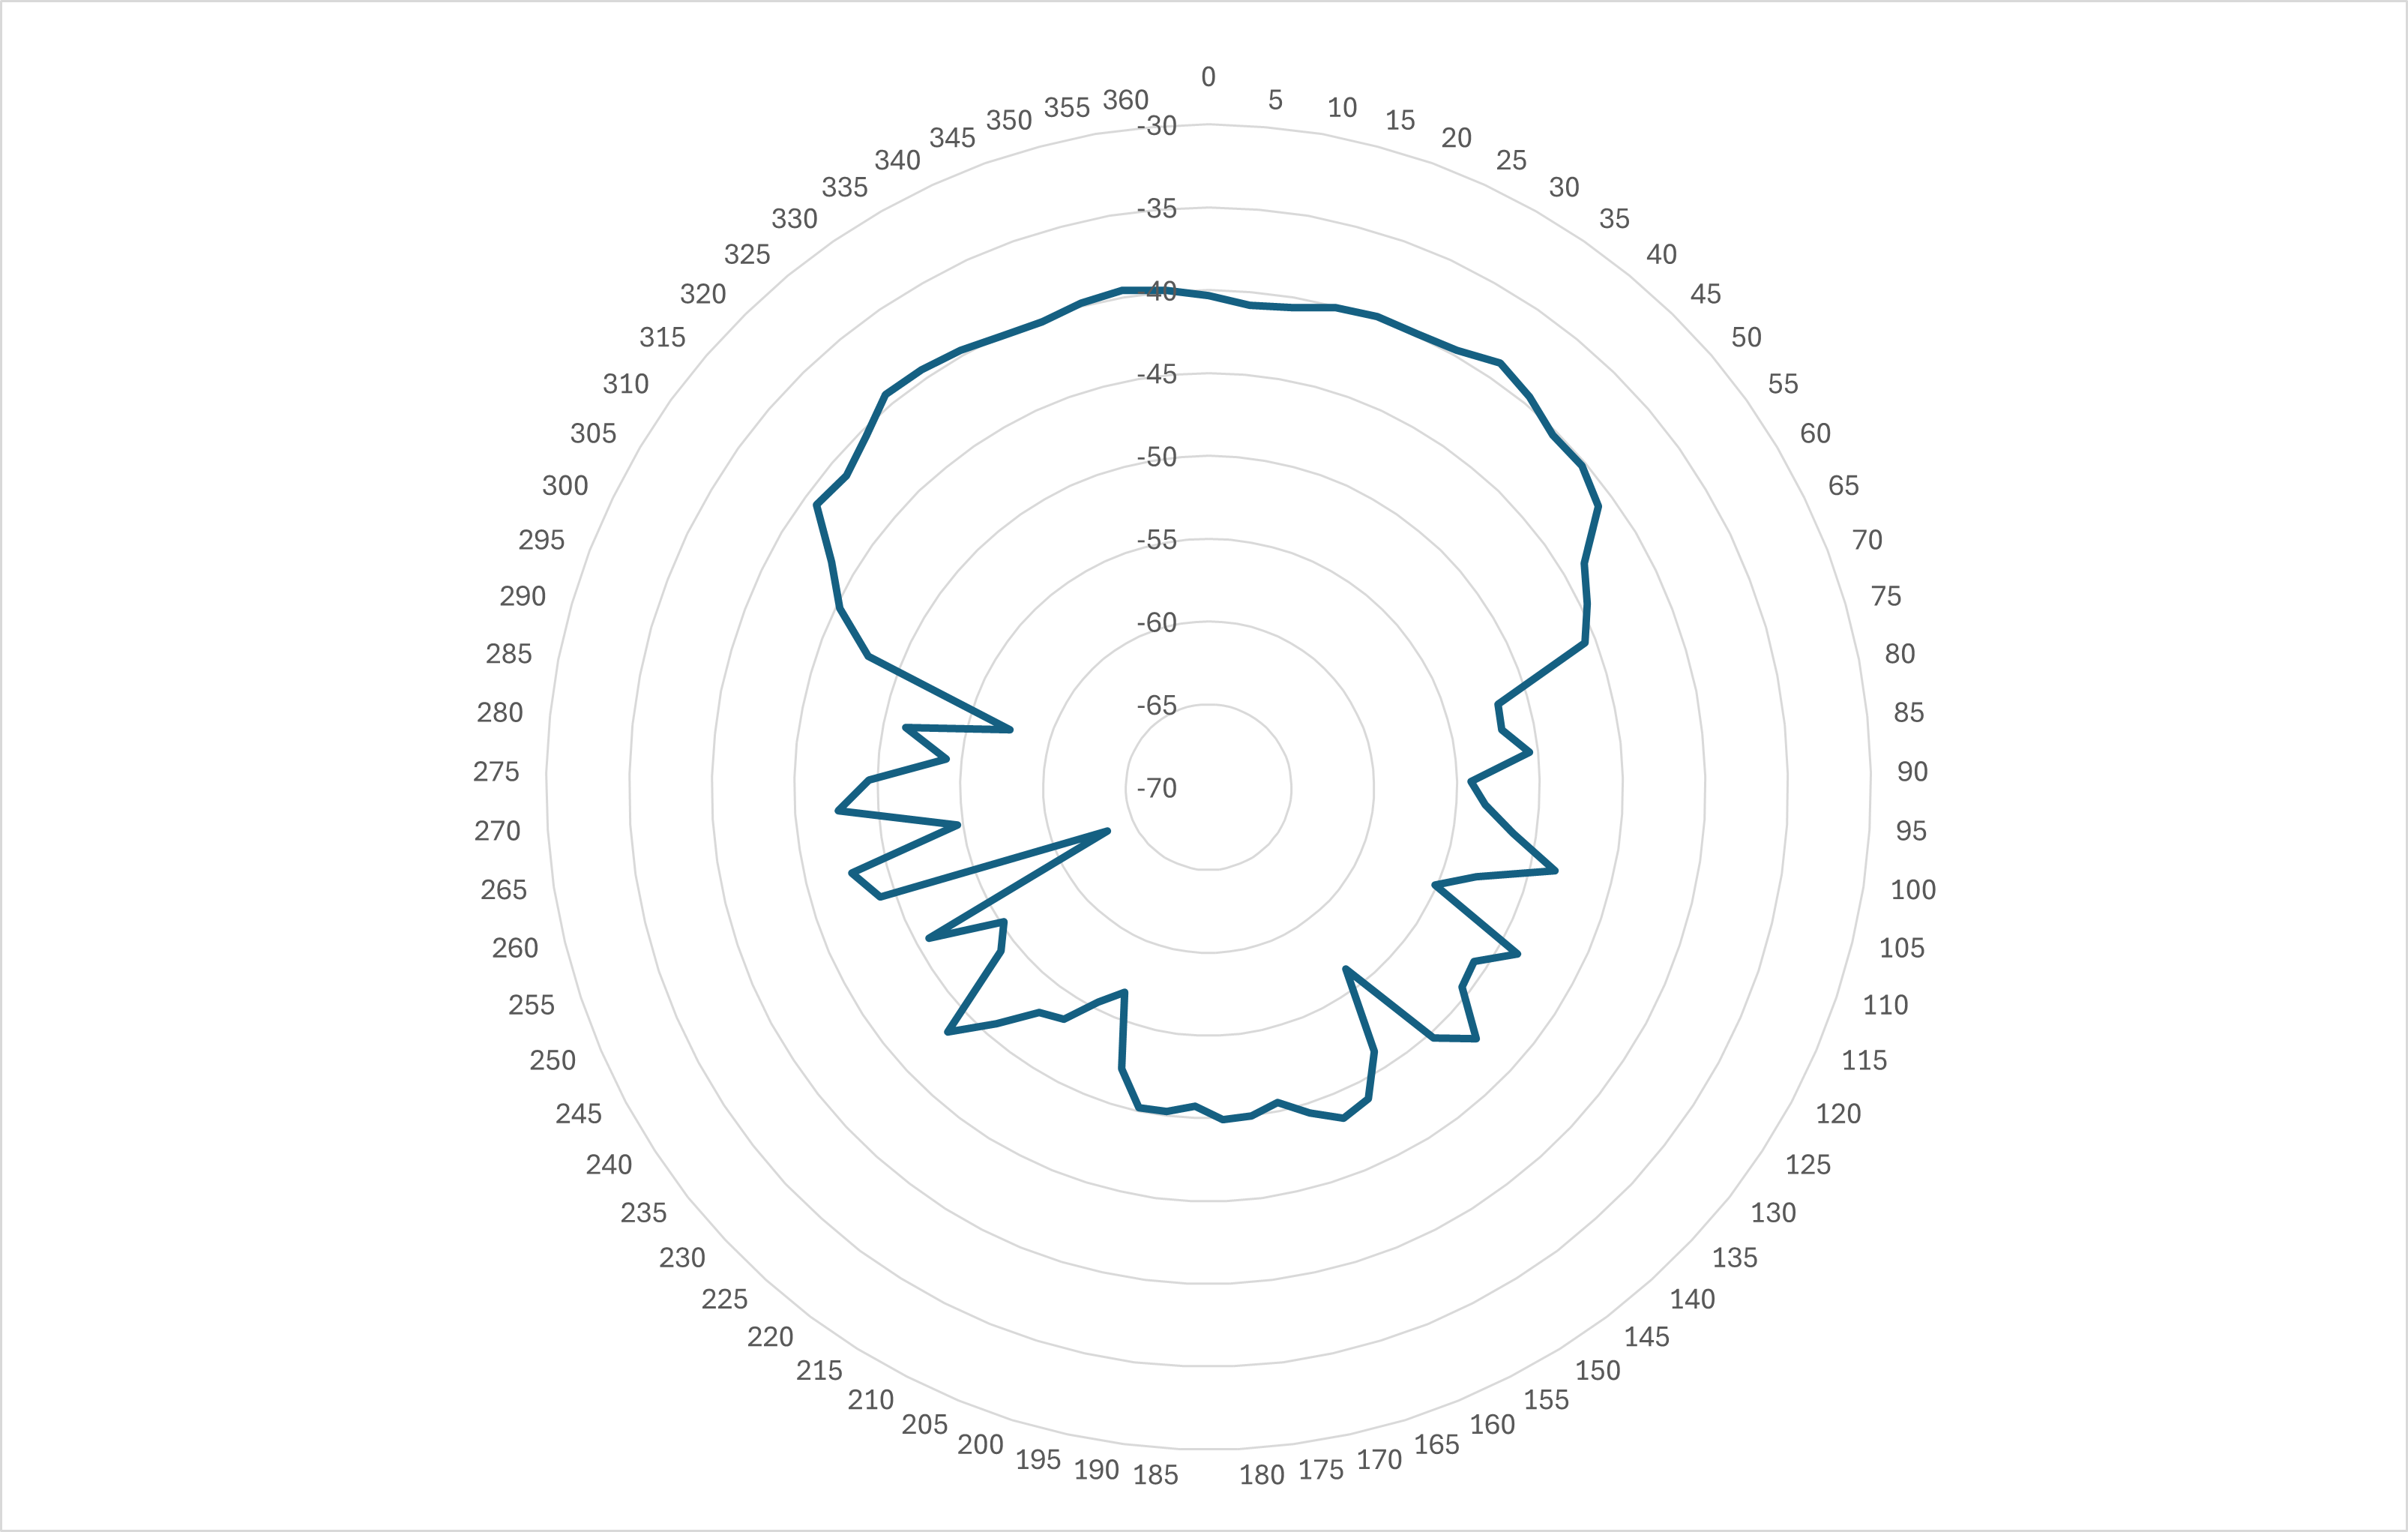
\includegraphics[scale=0.5]{pics/bab4/Ukur Pola Antena 23 Juli/S21A1.png}
	\caption{Hasil pengukuran pola radiasi antena}
	\label{fig:polaRadiasi}
\end{figure}

Gambar~\ref{fig:polaRadiasi} menunjukkan pola radiasi yang bagus untuk digunakan dalam implementasi radar, hal ini ditunjukkan dengan jenis pola radiasi \textit{directional} ke derajat 0. Selain itu, nilai gain dari antena yang digunakan adalah 6 dBi sesuai dengan datasheet yang ada dari antena.

%-----------------------------------------------------------------------------%
\section{Pengambilan Data Jarak}
%-----------------------------------------------------------------------------%

Pengambilan data jarak dilakukan di lapangan upacara Universitas Telkom Surabaya dengan menggunakan kendaraan roda dua. Dengan menggunakan pita ukur dan mengatur jarak kendaraan sesuai dengan parameter pengukuran, pengambilan data jarak dapat dilakukan dengan lancar. Terdapat 3 variasi jarak yang dilakukan, masing masing diulang sebanyak 3 kali untuk menjadi validasi.

\subsection{Jarak 3 Meter}

Pengambilan data jarak 3 meter yang dihitung dari ujung antena hingga ke kendaraan roda dua telah dilakukan seperti pada gambar~\ref{fig:pengambilan3Meter}. Untuk memastikan isolasi antara antena \textit{transmitter} dan antena \textit{receiver}, maka digunakanlah plat yang terbuat dari logam.

\begin{figure}
	\centering
	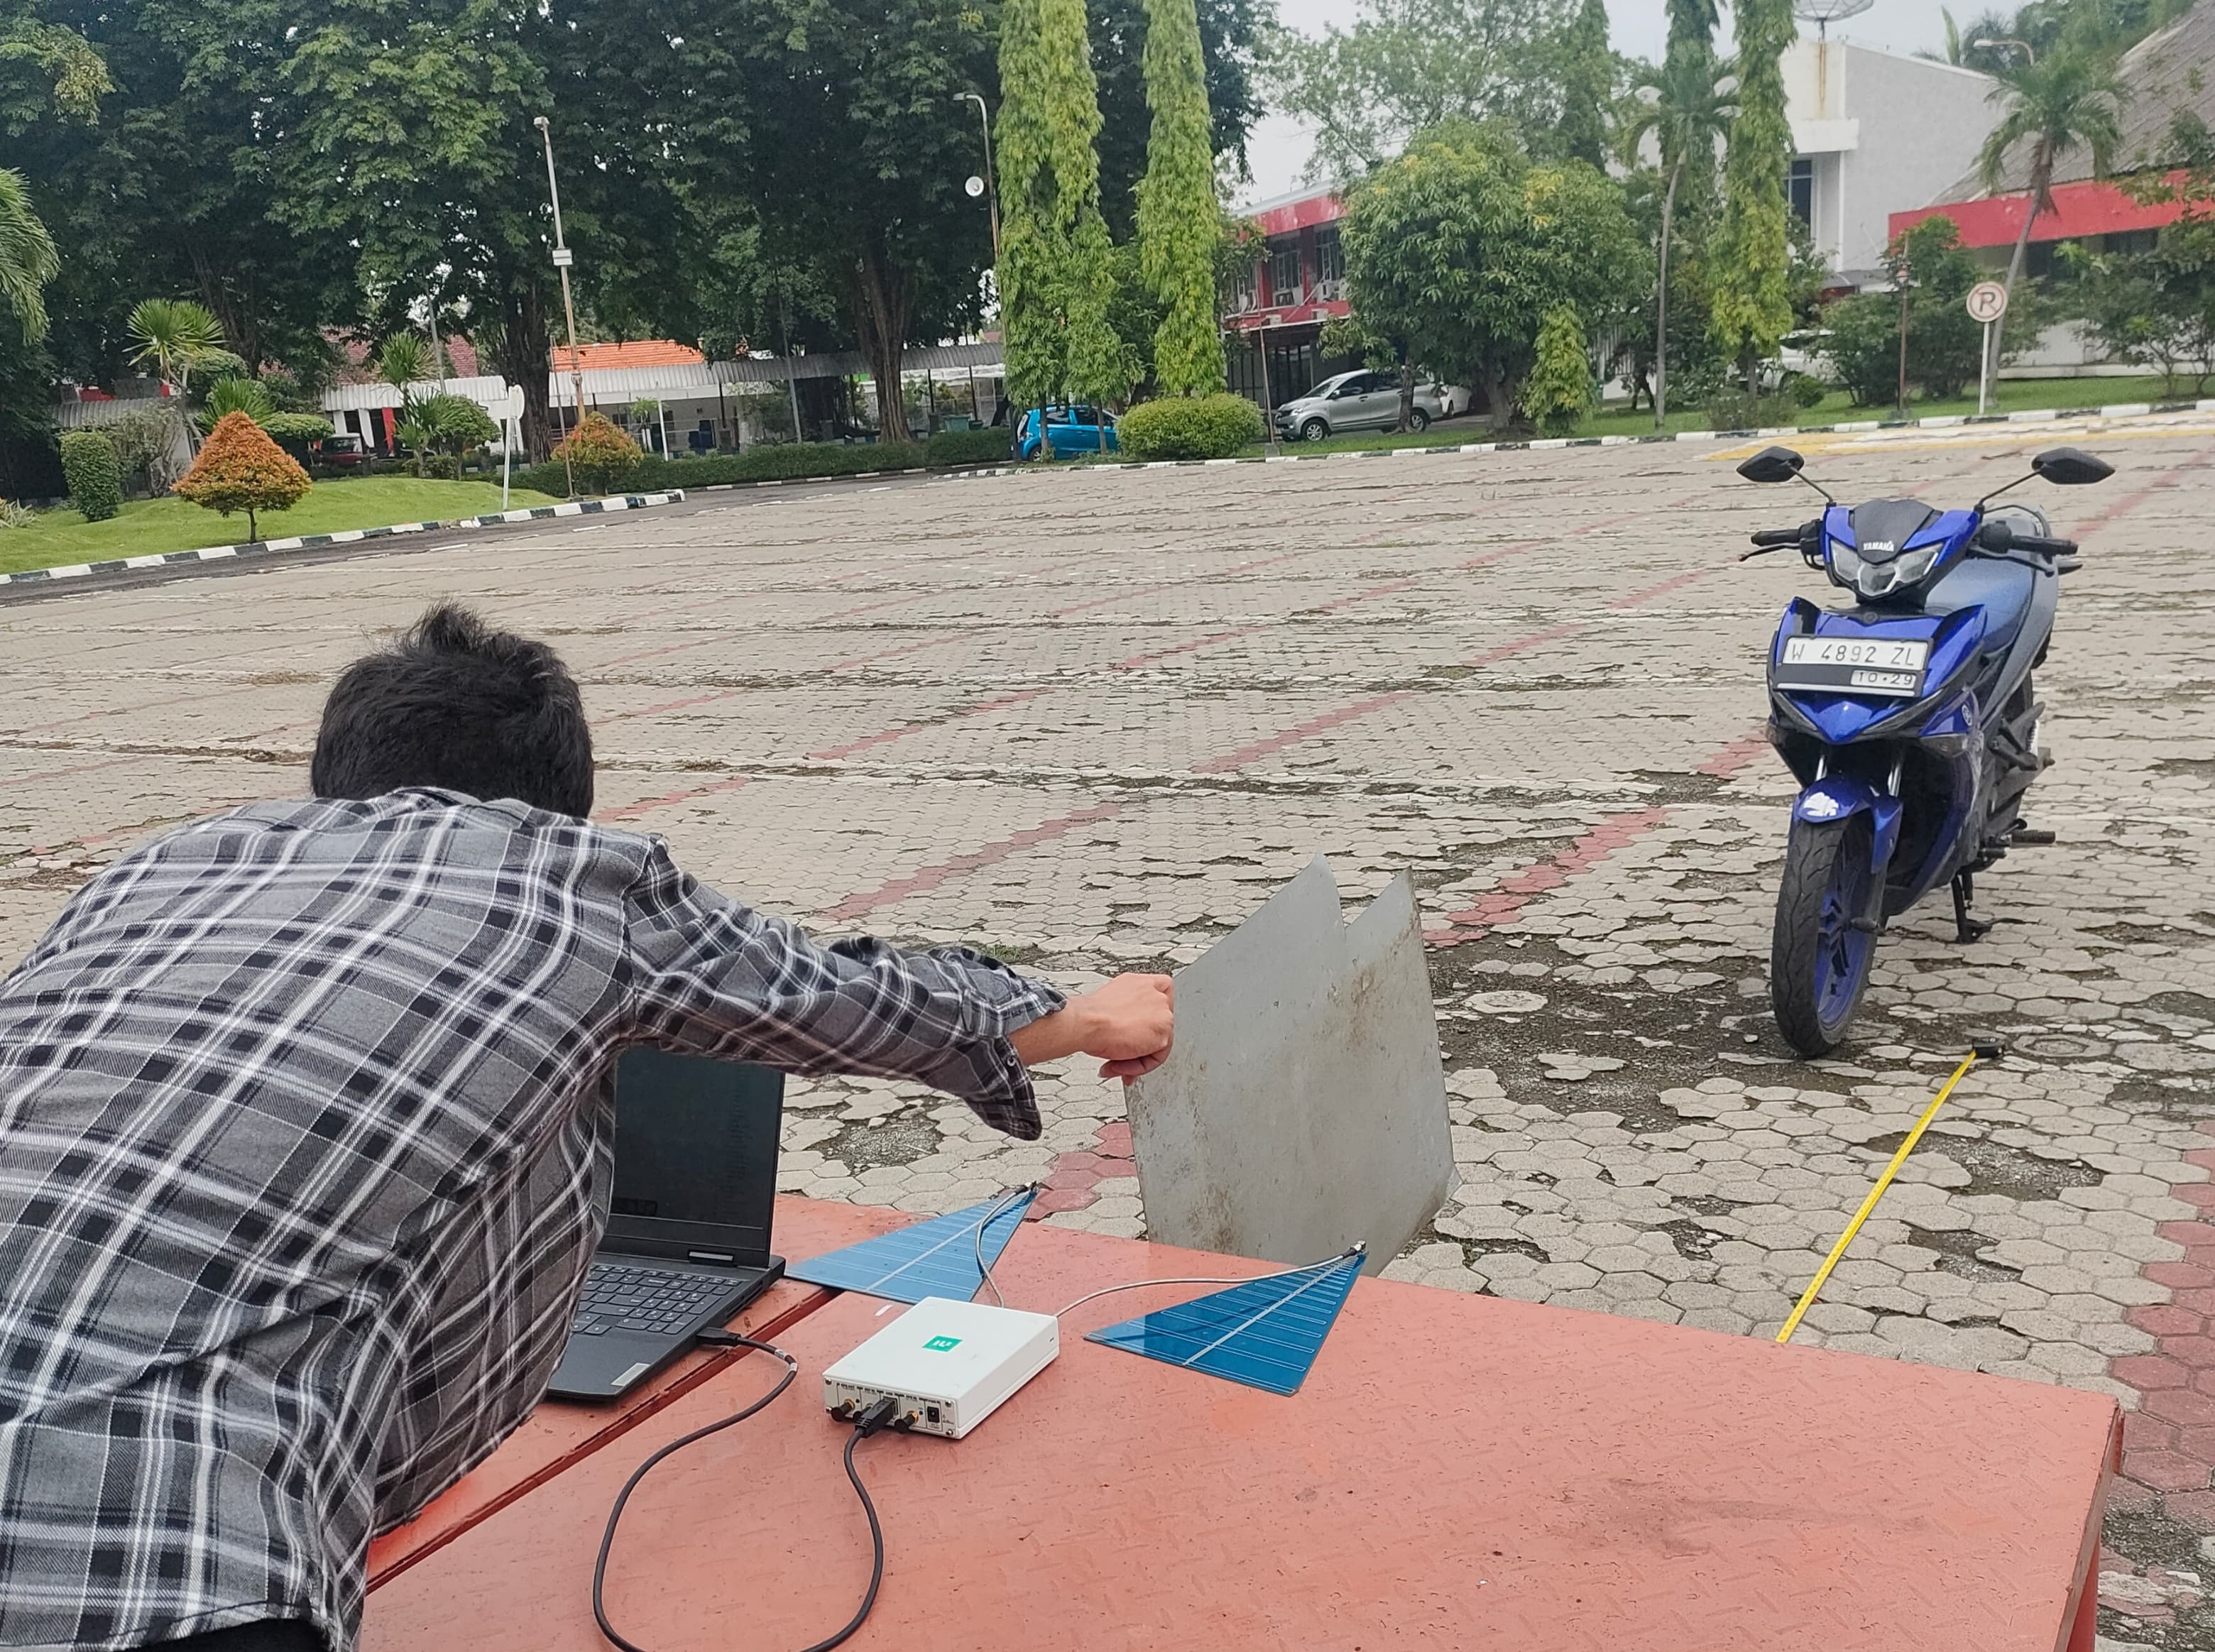
\includegraphics[scale=0.1]{pics/bab4/PengujianRange/3/Masuk.jpg}
	\caption{Pengambilan data jarak 3 meter}
	\label{fig:pengambilan3Meter}
\end{figure}

\subsection{Jarak 6 Meter}

Pengambilan data jarak 6 meter yang juga dilakukan dilokasi yang sama telah dilakukan. Dengan skema perhitungan jarak yang sama dengan pengambilan data jarak 3 meter. Namun pada jarak ini kesulitan dalam mengukur jarak dari ujung antena ditemui karena batas pita ukur yang hanya 3 meter, maka dari itu, pengukuran jarak dilakukan dimulai dari titik sebelumnya yaitu 3 meter.

\begin{figure}
	\centering
	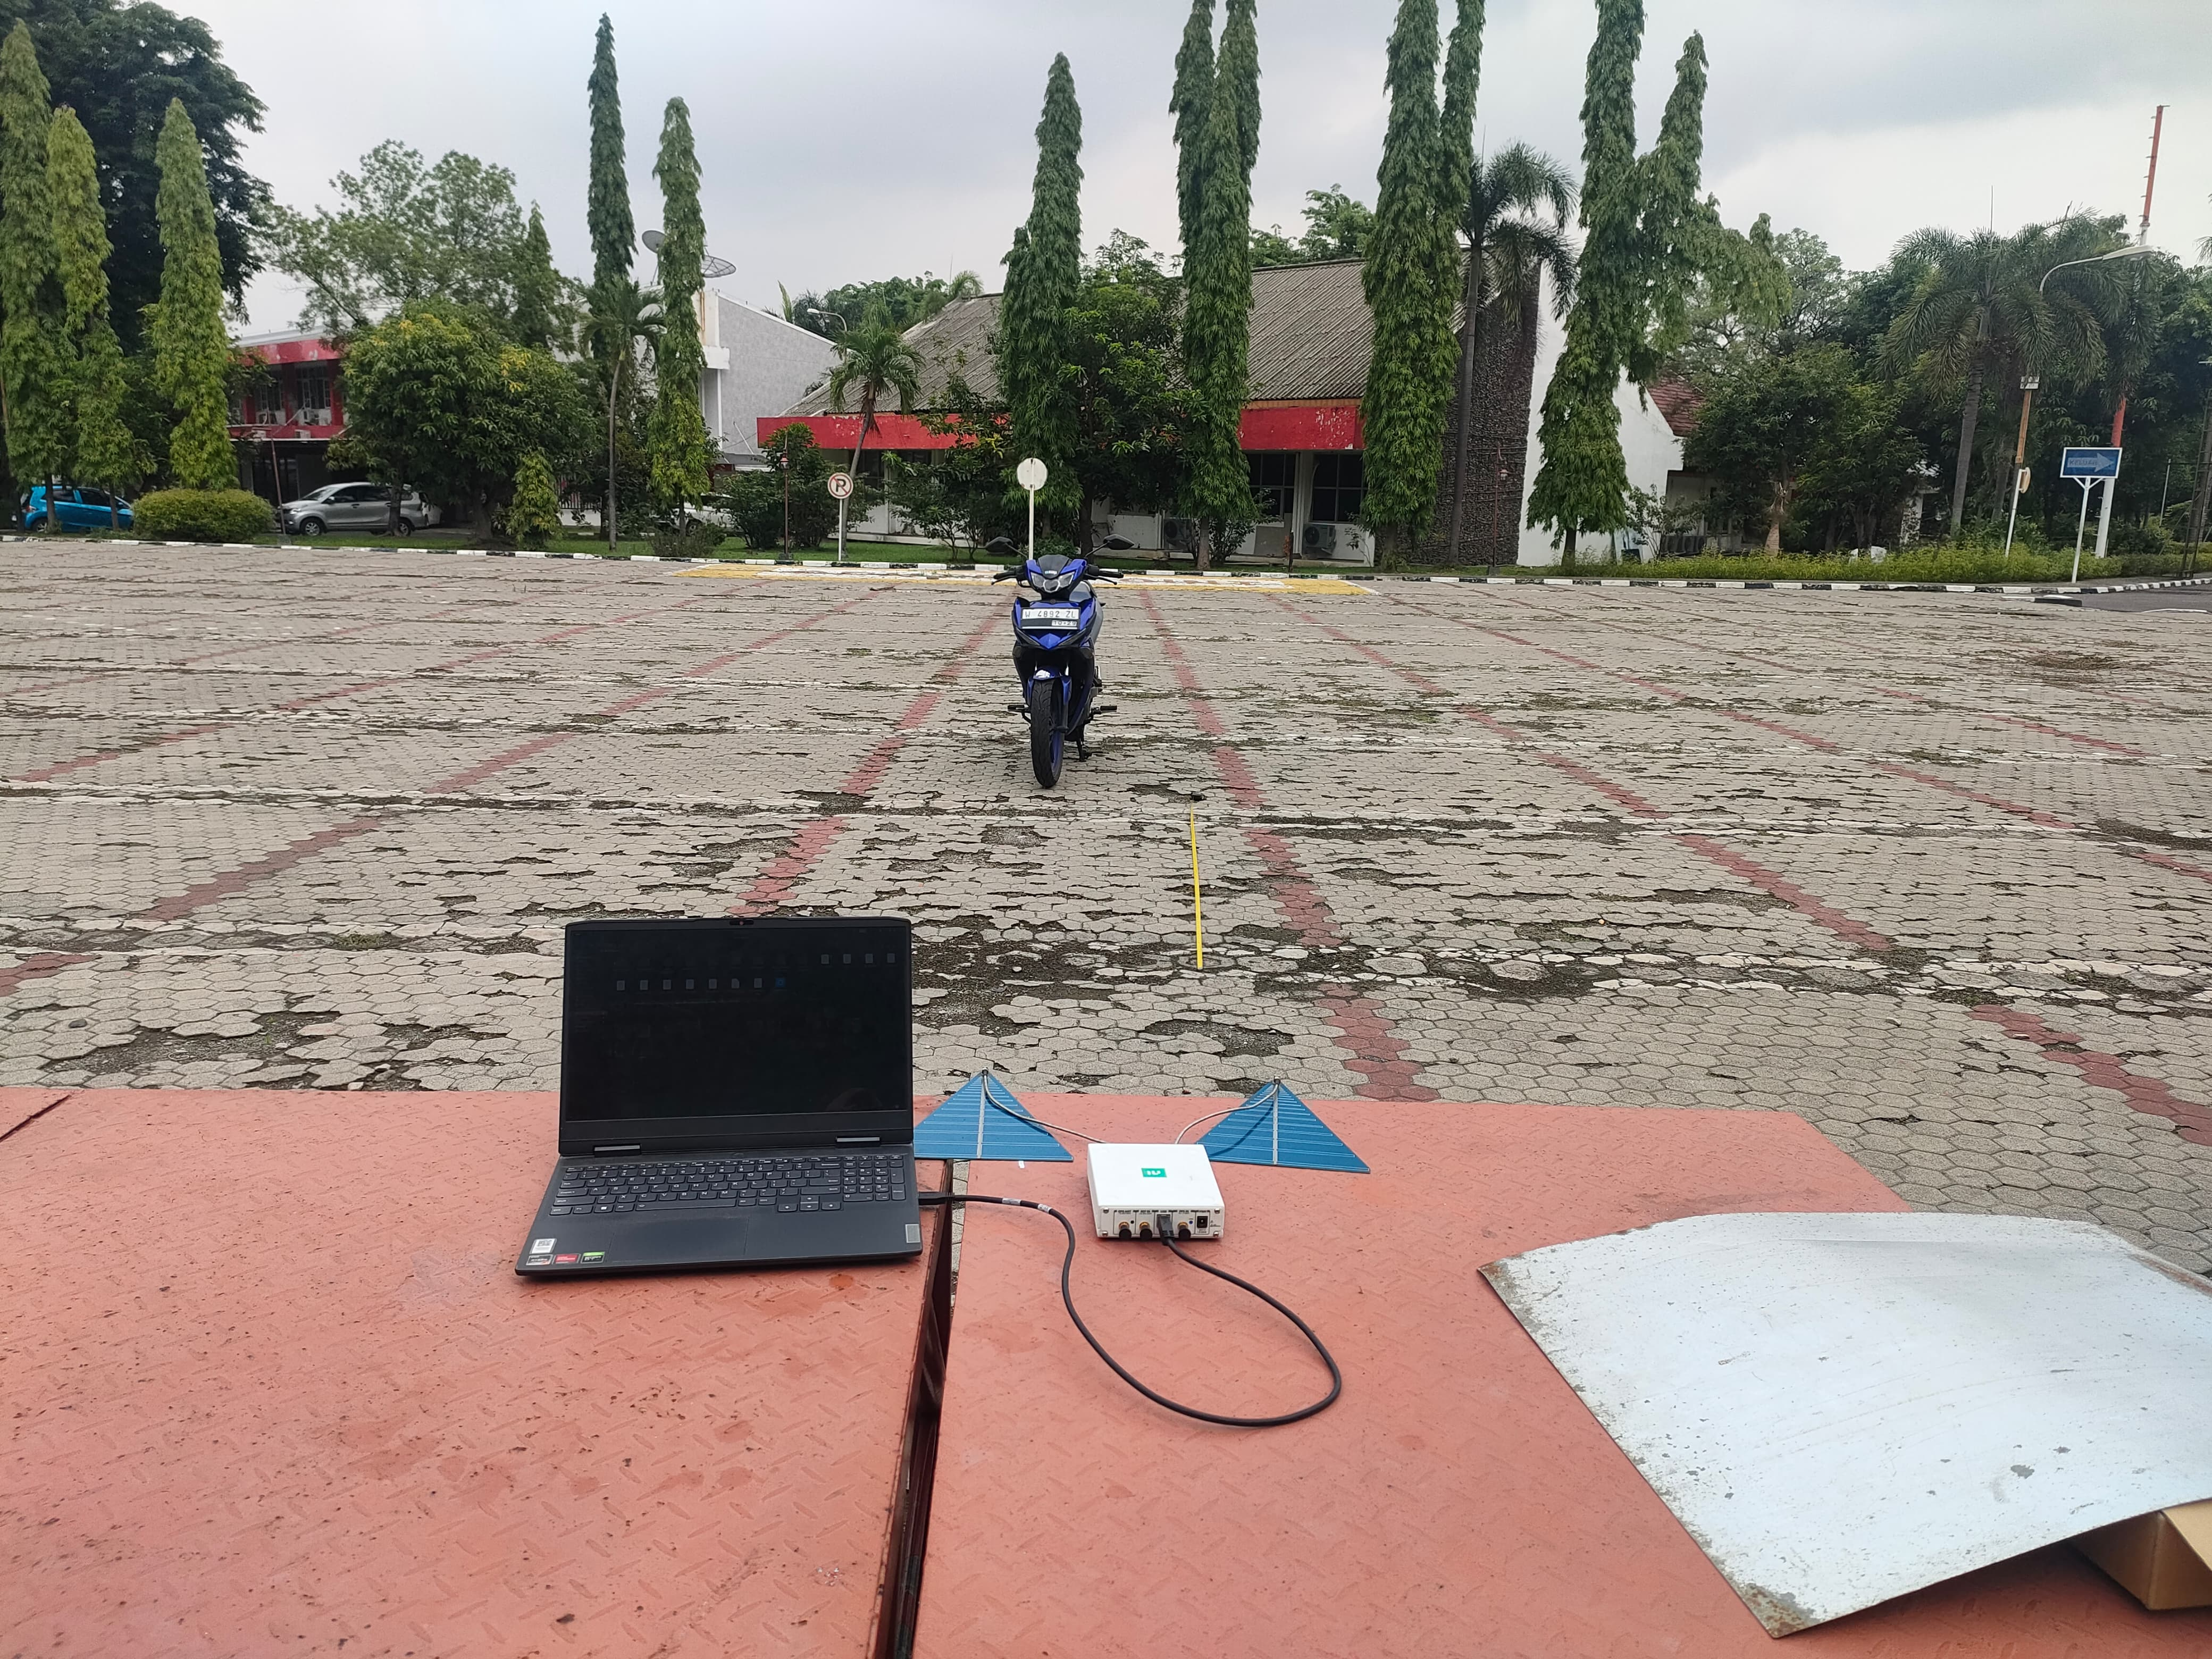
\includegraphics[scale=0.07]{pics/bab4/PengujianRange/6/Masuk.jpg}
	\caption{Pengambilan data jarak 6 meter}
	\label{fig:pengambilan6Meter}
\end{figure}

\subsection{Jarak 9 Meter}

Pengambilan data jarak 9 meter dari ujung antena telah dilaksanakan dengan lancar. Skema pengambilan data jarak sama dengan pengambilan data pada jarak 6 meter. Yaitu dengan memulai perhitungan titik mulai ukur dari titik jarak 6 meter dari antena.

\begin{figure}
	\centering
	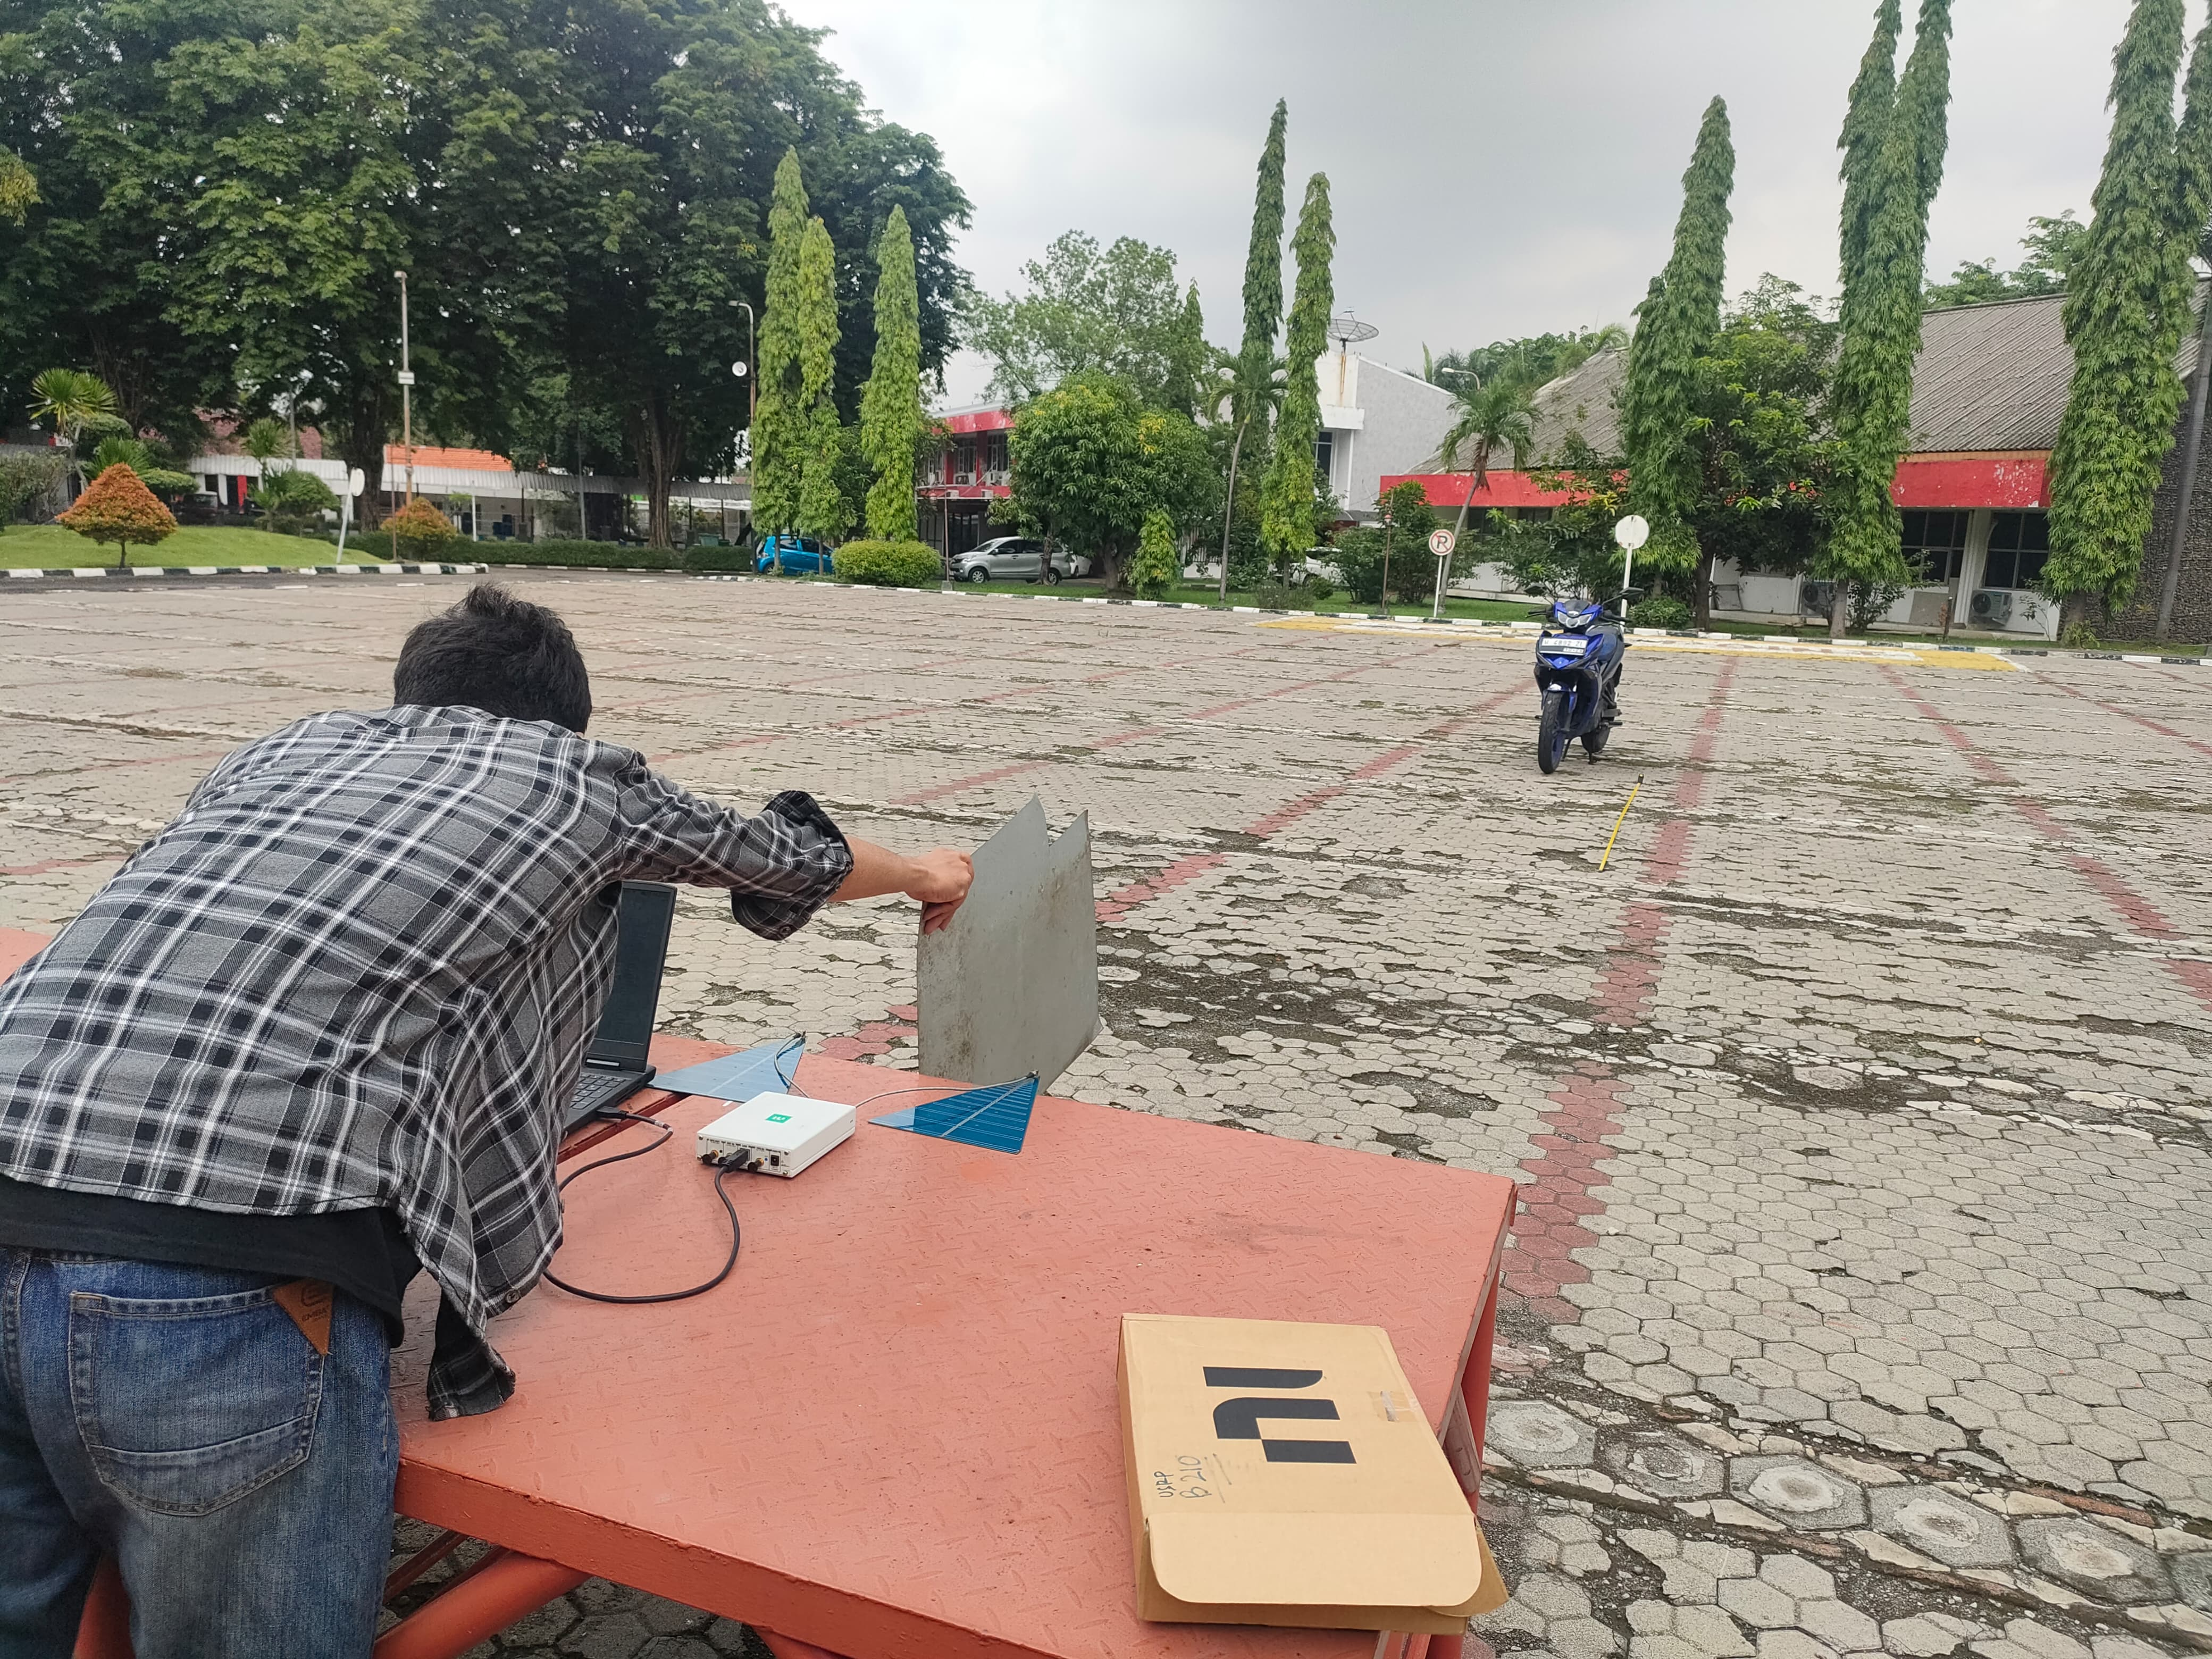
\includegraphics[scale=0.07]{pics/bab4/PengujianRange/9/Masuk.jpg}
	\caption{Pengambilan data jarak 9 meter}
	\label{fig:pengambilan9Meter}
\end{figure}
%-----------------------------------------------------------------------------%
\section{Pengambilan Data Kecepatan}
%-----------------------------------------------------------------------------%

Pengambilan data kecepatan dari objek dilakukan di tempat yang berbeda dengan pengambilan data jarak. Hal ini dikarenakan lintasan yang ada di lokasi pengambilan jarak tidak mendukung kecepatan hingga 20 km/h. Sehingga diputuskan bahwa pengambilan data kecepatan harus dilakukan ditempat lain yang memiliki lintasan mulus dan tidak membahayakan. Berbeda dengan pengambilan data jarak, pada data kecepatan diambil 2 skema yaitu mendekati radar dan menjauhi radar dengan 4 variasi kecepatan, masing masing kecepatan yang diuji dilakukan pengulangan sebanyak 3 kali. 

\subsection{Menjauhi Radar}

Pengambilan data menjauhi radar dilakukan dengan mengendarai kendaraan roda dua dekat dengan antena radar lalu melaju dengan kecepatan yang sudah ditentukan seperti pada gambar~\ref{fig:pengambilanMenjauhi}. Data akan terus diambil hingga 10 detik telah berlalu. Pembatasan pengambilan data ini dilakukan karena semakin lama data diambil, maka semakin besar pula data yang dihasilkan, sehingga pengolahan akan semakin berat untuk dilakukan.

\begin{figure}
	\centering
	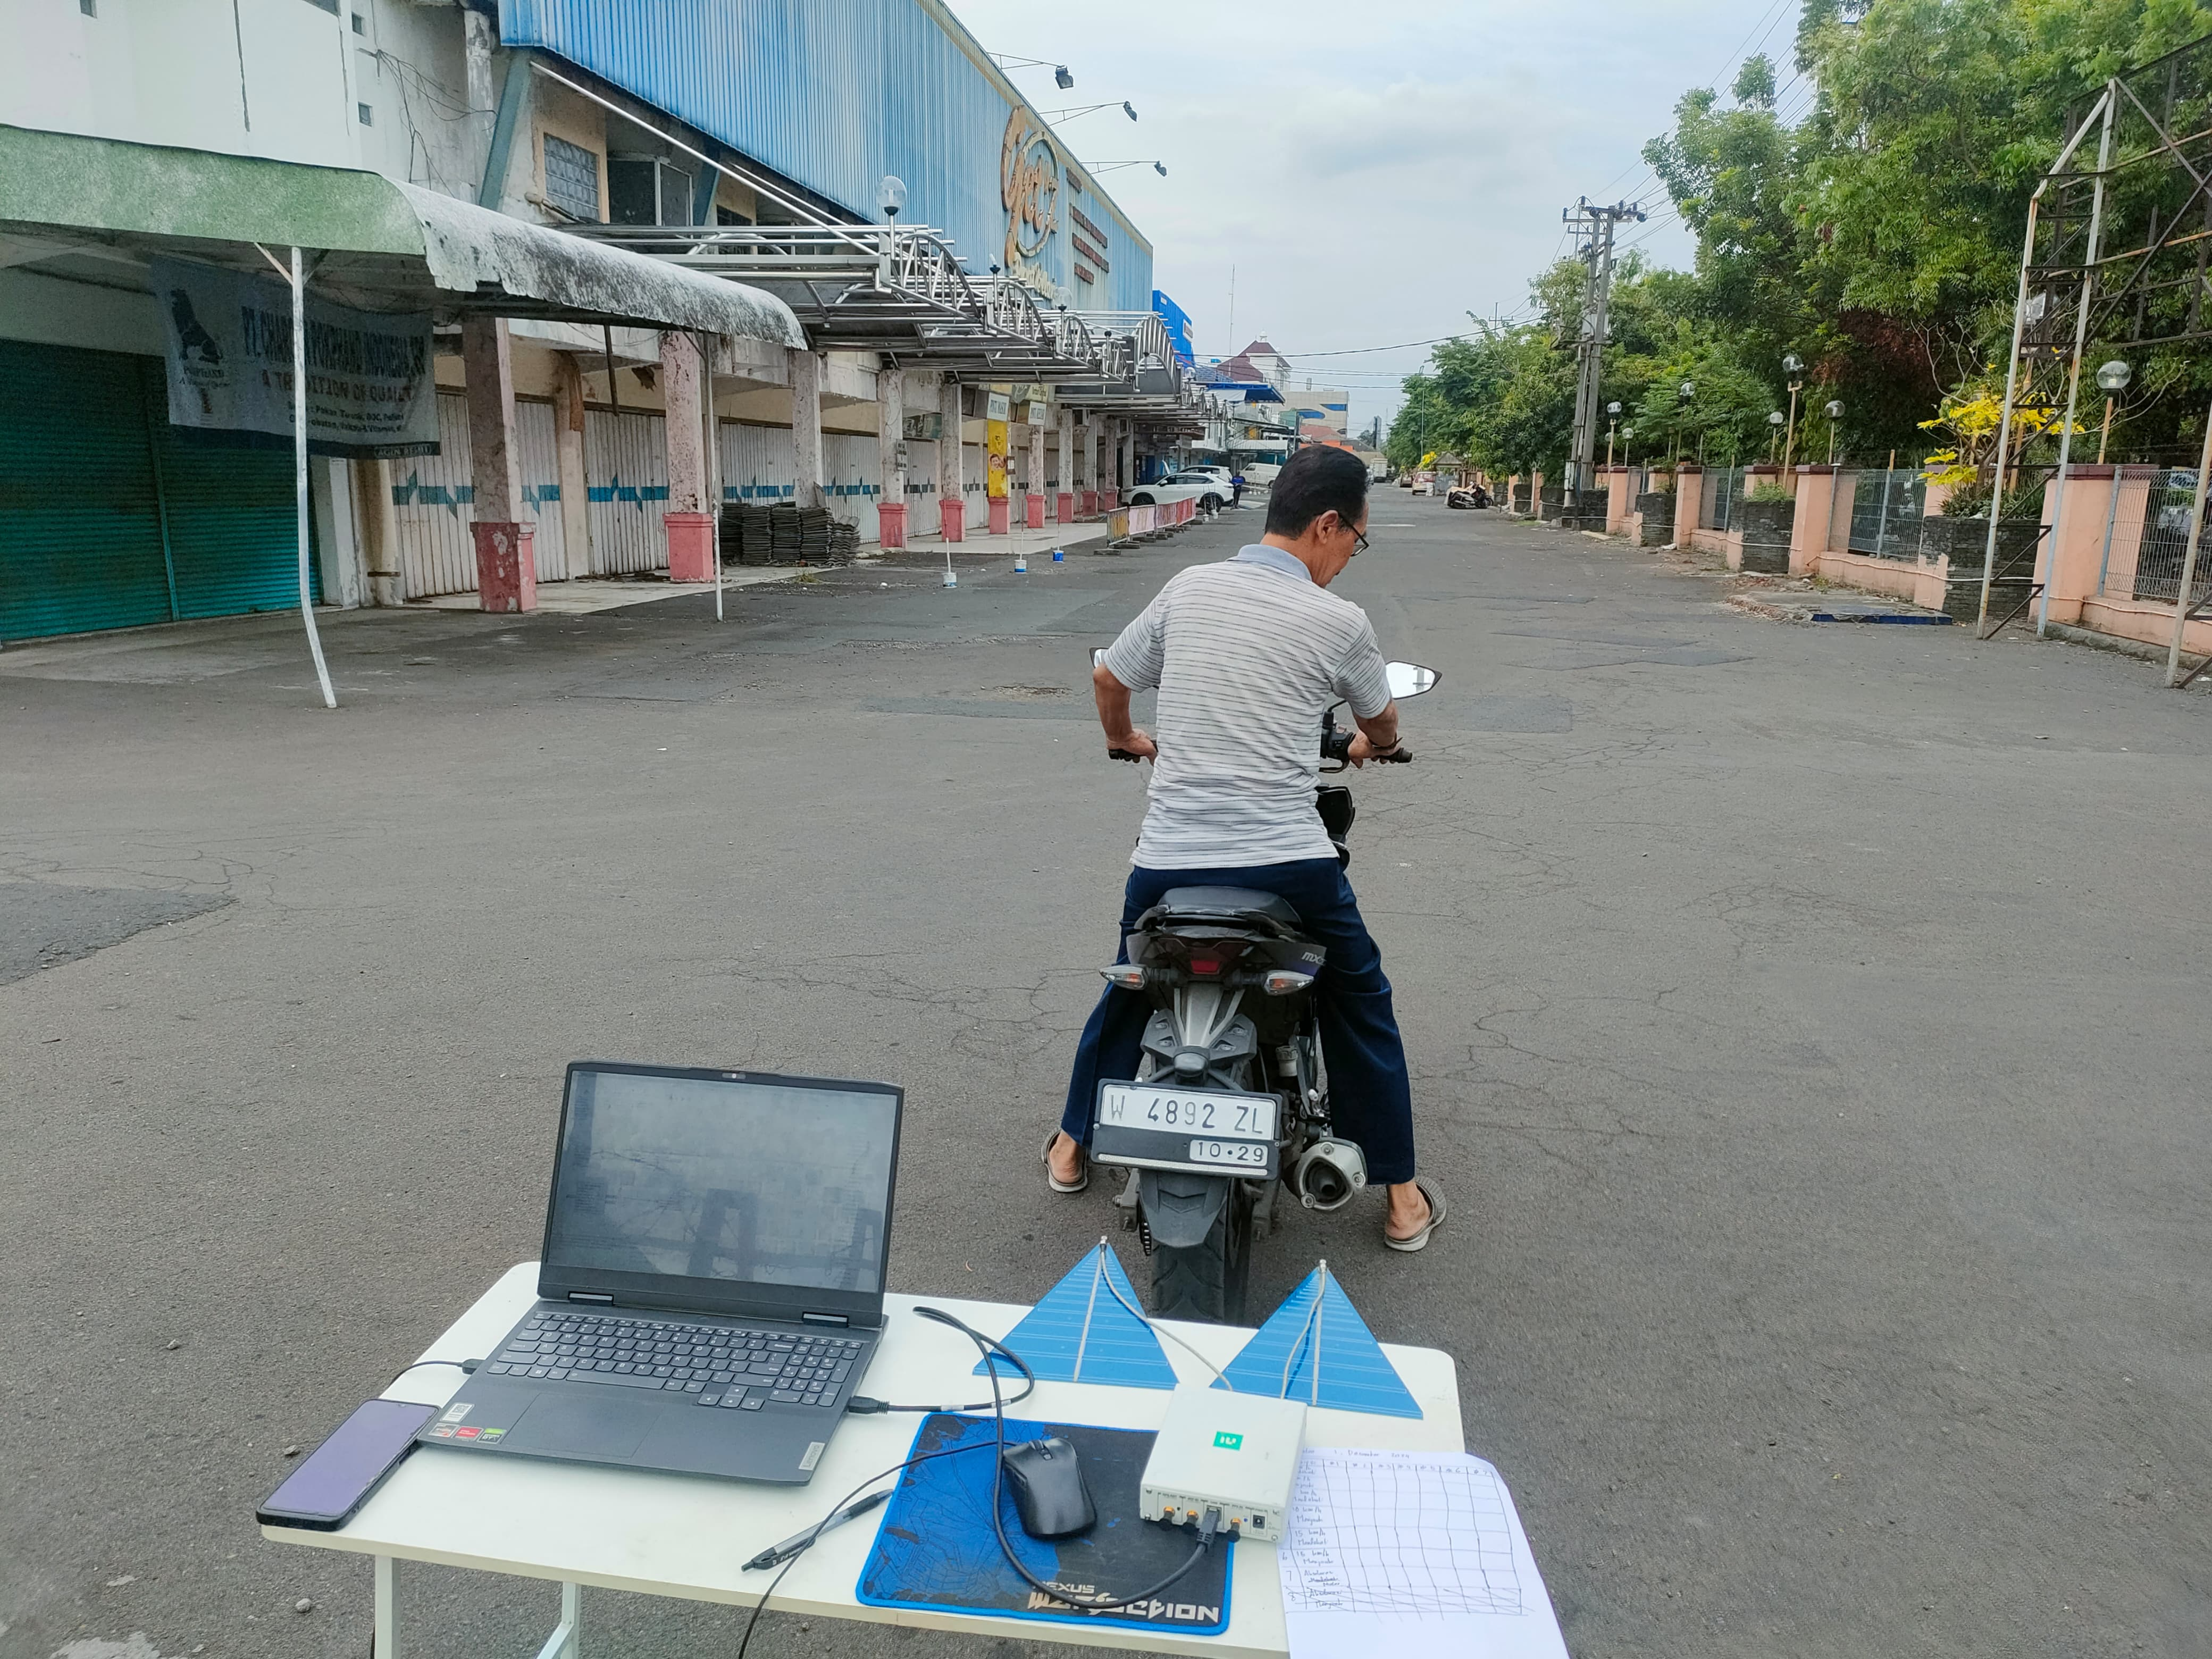
\includegraphics[scale=0.07]{pics/bab4/PengujianVelocity/1.jpg}
	\caption{Pengambilan data kecepatan menjauhi radar}
	\label{fig:pengambilanMenjauhi}
\end{figure}

\subsection{Mendekati Radar}

Pengambilan data mendekati radar dilakukan hampir sama dengan skema menjauhi radar, hanya saja jarak awal kendaraan ada pada sekitar 20 meter dari antena radar. Namun pemilihan jarak awal ini berubah, tiap kecepatan yang dipilih, pada pengukuran kecepatan lebih lambat, jarak awal yang dipilih lebih dekat dibanding kecepatan lebih tinggi. Hal ini dilakukan untuk memastikan kecepatan dari kendaraan bisa stabil di angka yang telah ditentukan. Gambar~\ref{fig:pengambilanMendekati} menunjukkan kegiatan pengambilan data yang telah dilaksanakan.

\begin{figure}
	\centering
	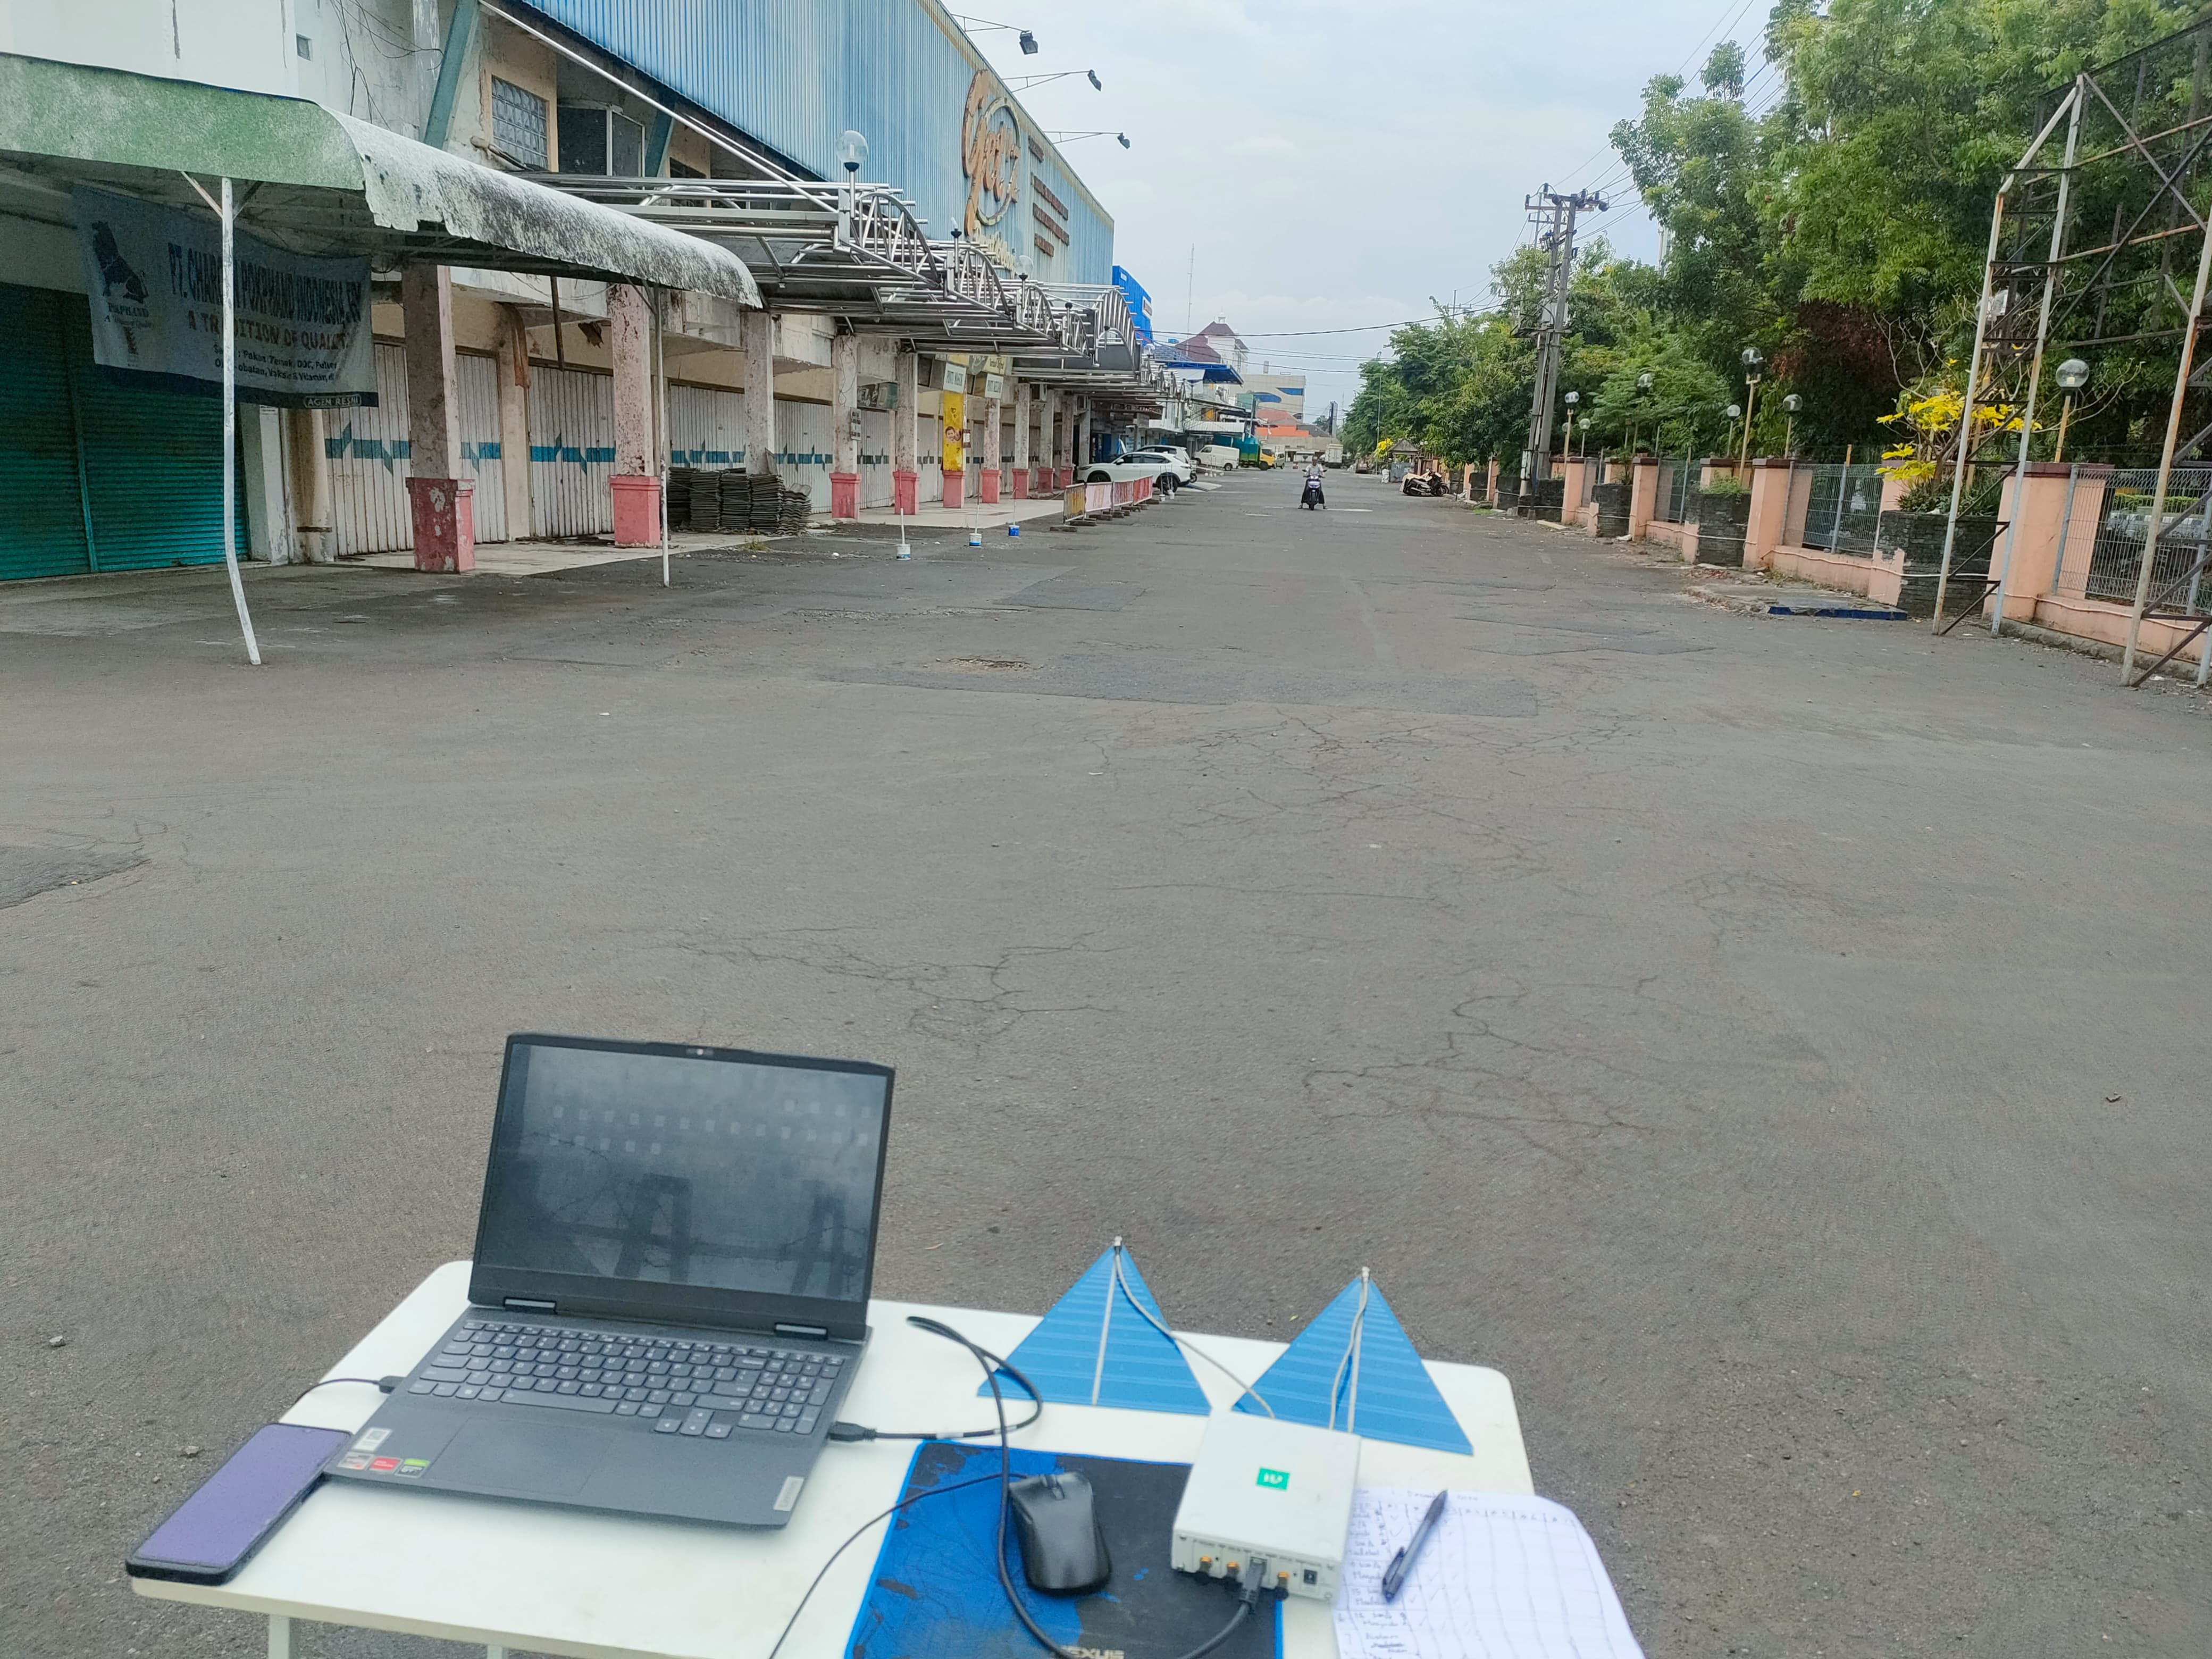
\includegraphics[scale=0.07]{pics/bab4/PengujianVelocity/3.jpg}
	\caption{Pengambilan data kecepatan mendekati radar}
	\label{fig:pengambilanMendekati}
\end{figure}

%-----------------------------------------------------------------------------%
\section{Pengolahan Data Dengan Matlab}
%-----------------------------------------------------------------------------%

Setelah dilaksanakan pengambilan data jarak objek dan kecepatan objek, selanjutnya adalah melakukan pengolahan dengan perangkat lunak matlab.

\subsection{Pengolahan Data Jarak}

Data jarak yang sudah didapat akan diolah dengan perangkat lunak matlab. Dengan melakukan perkalian \textit{conjugate} antara sinyal terkirim dan sinyal yang diterima, maka \textit{beat frequency} akan didapat. Saat nilai \textit{beat frequency} didapat, maka selanjutnya nilai tersebut bisa dimasukkan kedalam persamaan~\ref{eq:RangeEst}. Persamaan ini telah tersedia dalam bentuk fungsi di dalam perangkat lunak matlab, dengan memanggil \textit{beat2range(fb,slope)} dimana fb adalah nilai \textit{beat frequency} yang didapat dari pengolahan sebelumnya dan \textit{slope} adalah lebar \textit{sweep bandwidth} yang telah dipilih, yaitu 14 MHz. 

\subsection{Pengolahan Data Kecepatan}

Data kecepatan secara teori dilakukan dengan mengukur berapa pergeseran frekuensi yang terjadi antara frekuensi terkirim dan frekuensi yang diterima. Namun pada kenyataannya, data yang didapat memiliki \textit{phase noise}, seperti yang ditunjukkan pada gambar~\ref{fig:phaseNoise}. 

\begin{figure}
	\centering
	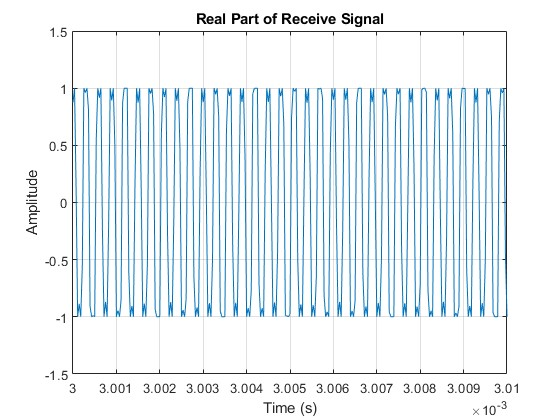
\includegraphics[scale=0.5]{pics/bab4/RealPartRx.jpg}
	\caption{\textit{Phase Noise} dari sinyal yang diterima}
	\label{fig:phaseNoise}
\end{figure}

Gambar~\ref{fig:phaseNoise} menunjukkan bagian real dari sinyal FMCW yang terpantul dari objek. Dapat dilihat pada fasa 90, selalu terjadi kerusakan sinyal, perlu diingat bahwa pengamatan sinyal ini dilakukan dalam waktu 0.01 detik. Saat seluruh sinyal diterima di plot dalam bentuk perubahan frekuensi dalam waktu, hal ini akan terlihat dengan jelas seperti dalam gambar~\ref{fig:instFreq}.

\begin{figure}
	\centering
	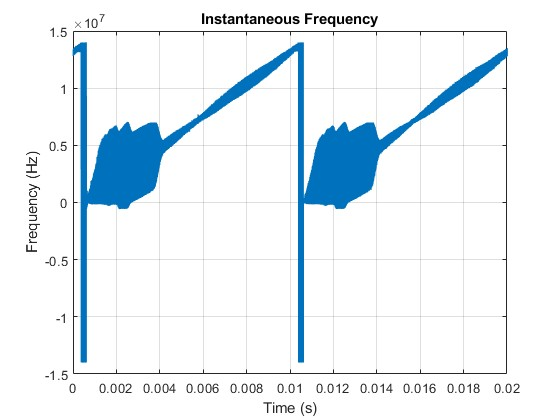
\includegraphics[scale=0.5]{pics/bab4/InstFreq.jpg}
	\caption{Perubahan frekuensi dengan waktu}
	\label{fig:instFreq}
\end{figure}

Nampak pada gambar~\ref{fig:instFreq} bahwa selalu ada \textit{phase noise} yang terjadi, sehingga saat sinyal yang di transmisi dan sinyal yang diterima dibandingkan, pengukuran kecepatan akan sangat sulit dilaksanakan, apalagi saat sinyal doppler yang terjadi sangat kecil. Sehingga digunakanlah teknik lain dalam mengukur kecepatan. Kecepatan dapat didefinisikan menggunakan persamaan sederhana kecepatan bersimbol V, dengan S dibagi t. S adalah jarak tempuh objek dan t adalah waktu tempuh objek. Dengan melakukan konversi dari minimal dua \textit{beat frequency} ke dalam jarak, dan melakukan kalkulasi terhadap perubahan waktu tersebut, maka nilai kecepatan akan didapat.

%\begin{equation}
%	V = \frac{S}{t}
%\end{equation}

 


%%--------------------------------%
%\todo{
	%\section{Simulasi Sistem}
	%Masukkan gambar simulasi pada gnuradio\\ 
	%Masukkan gambar hasil yang dilakukan dengan simulasi (berupa time vs frequency).\\
	%Masukkan proses analisis yang dilakukan dengan hasil simulasi, seperti langkah konversi biner ke kompleks, penentuan data yang diambil,... pada matlab.\\
	%Lakukan desain blok dari hasil pada matlab menuju python.\\
	%Uji coba blok python yang telah dirancang pada simulasi\\
	%Bandingkan hasilnya dengan pada matlab
	%}
%%--------------------------------%

% Bab 5 : Analisis dan Pembahasan
%---------------------------------------------------------------
\chapter{\babLima}
%---------------------------------------------------------------

%---------------------------------------------------------------
\section{Kesimpulan}
%---------------------------------------------------------------

%---------------------------------------------------------------
\section{Saran}
%---------------------------------------------------------------

% Bab 6 : Kesimpulan dan Saran
%---------------------------------------------------------------
\chapter{\babEnam}
%---------------------------------------------------------------
%---------------------------------------------------------------
\section{Kesimpulan}
%---------------------------------------------------------------

Pada bagian ini, kesimpulan dari penelitian akan disajikan. Terutama dalam menjawab rumusan masalah yang diajukan pada penelitian ini, maka kesimpulan yang diperoleh adalah:

\begin{enumerate}
    \item Perancangan sistem radar FMCW dengan GNURadio telah dilakukan dengan menggunakan kemampuan maksimal dari USRP B210. Mulai dari frekuensi sampling 28 MHz bagi \textit{transmit} dan \textit{receive}, lalu lebar \textit{bandwidth} 14 MHz, hingga nilai \textit{internal gain} maksimum untuk mencapai jarak paling jauh yang dapat dicakup. Sistem telah dirancang dan implementasikan dengan baik.
    \item Pengujian sistem radar FMCW telah dilakukan, khususnya untuk melakukan pendeteksi objek, estimasi jarak, dan kecepatan objek. Dengan menggunakan kendaraan roda dua yang memiliki \textit{Radar Cross Section} yang kecil, radar mampu menangkap sinyal pantulan dari objek.
    \item Evaluasi terhadap sistem radar FMCW yang didesain telah dilakukan setelah melakukan pengujian, didapatkan hasil bahwa radar bekerja dengan baik sebagai pendeteksi jarak yaitu pada 6 meter dengan nilai akurasi prediksi 82.86\% dan pada 9 meter dengan nilai akurasi sekitar 93.56\%. Sedangkan sistem radar yang didesain tidak dapat mendeteksi objek pada jarak 3 meter dengan nilai akurasi -402.72\%. Dalam pengujian kecepatan, sistem radar yang didesain dapat melakukan estimasi kecepatan dengan perbandingan perubahan jarak. Dengan begitu maka radar dapat melakukan deteksi objek.
    %\item Dalam penelitian ini, langkah yang jelas telah dipaparkan dalam melakukan perancangan sistem radar FMCW dengan USRP B210 dan GNURadio. Dimulai dengan identifikasi kemampuan USRP, penyesuaian parameter sistem radar yang dirancang, prediksi kemampuan radar, implementasi sistem, dan pengujian radar.
\end{enumerate}

%---------------------------------------------------------------
\section{Saran}
%---------------------------------------------------------------

Dari penelitian yang sudah dilakukan, maka terdapat saran yang bisa di implementasikan pada penelitian selanjuntya.

\begin{enumerate}
    \item Menggunakan objek dengan \textit{Radar cross section} lebih besar untuk memastikan seluruh energi dapat terpantul secara maksimal oleh objek.
    \item Menggunakan perangkat keras lebih mumpuni untuk mengatasi \textit{error overflow} dan \textit{underflow} sehingga pengolahan data secara \textit{real time} dapat dilakukan.
    \item Menggunakan antena dengan \textit{beamwidth} lebih kecil dengan \textit{gain} tinggi untuk memastikan isolasi benar benar terjadi pada gelombang yang di transmisikan.
    \item Menggunakan teknik yang dapat memperbesar lebar pita dari sistem radar FMCW yang terbatas, seperti \textit{frequency hopping} dan \textit{synthetic wide-bandwidth}.
\end{enumerate}

% Daftar Pustaka
%
% Daftar Pustaka 
% 
% 
% Tambahkan pustaka yang digunakan setelah perintah berikut. 
% 
\renewcommand{\section}[2]{}%
\bibliographystyle{ieeetr}
\bibliography{dafpus}
 


%\bibliographystyle{plain}
%\bibliography{ref}

% Lampiran 
\begin{appendix}
	\pagenumbering{gobble}
	%
% @author  Andreas Febrian
% @version 1.00 
% 
% Hanya sebuah pembatas bertuliskan LAMPIRAN ditengah halaman. 
% 

\begin{titlepage}
	\centering 
	\vspace*{6cm}
	\noindent \Huge{LAMPIRAN}
	\addChapter{LAMPIRAN}
\end{titlepage}
	\setcounter{page}{2}
	%-----------------------------------------------------------------------------%
\addChapter{Lampiran 1}
\chapter*{Lampiran 1}
%-----------------------------------------------------------------------------%
\end{appendix}

\end{document}